\chapter{Extended Results} \label{ch:eresult}
\section{Set Estimation}
\FloatBarrier
\subsection{Segment Minimization using F-Radius}
\begin{figure}[!h]
\begin{subfigure}{.5\linewidth}
\centering
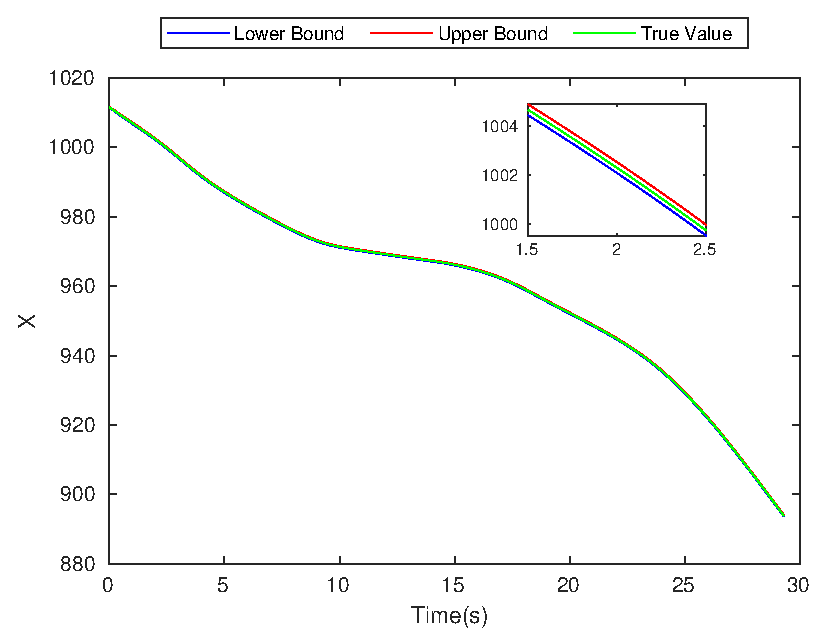
\includegraphics[width=\linewidth]{figures/Frad/s3cvSMX}
\end{subfigure}
\begin{subfigure}{.5\linewidth}
\centering
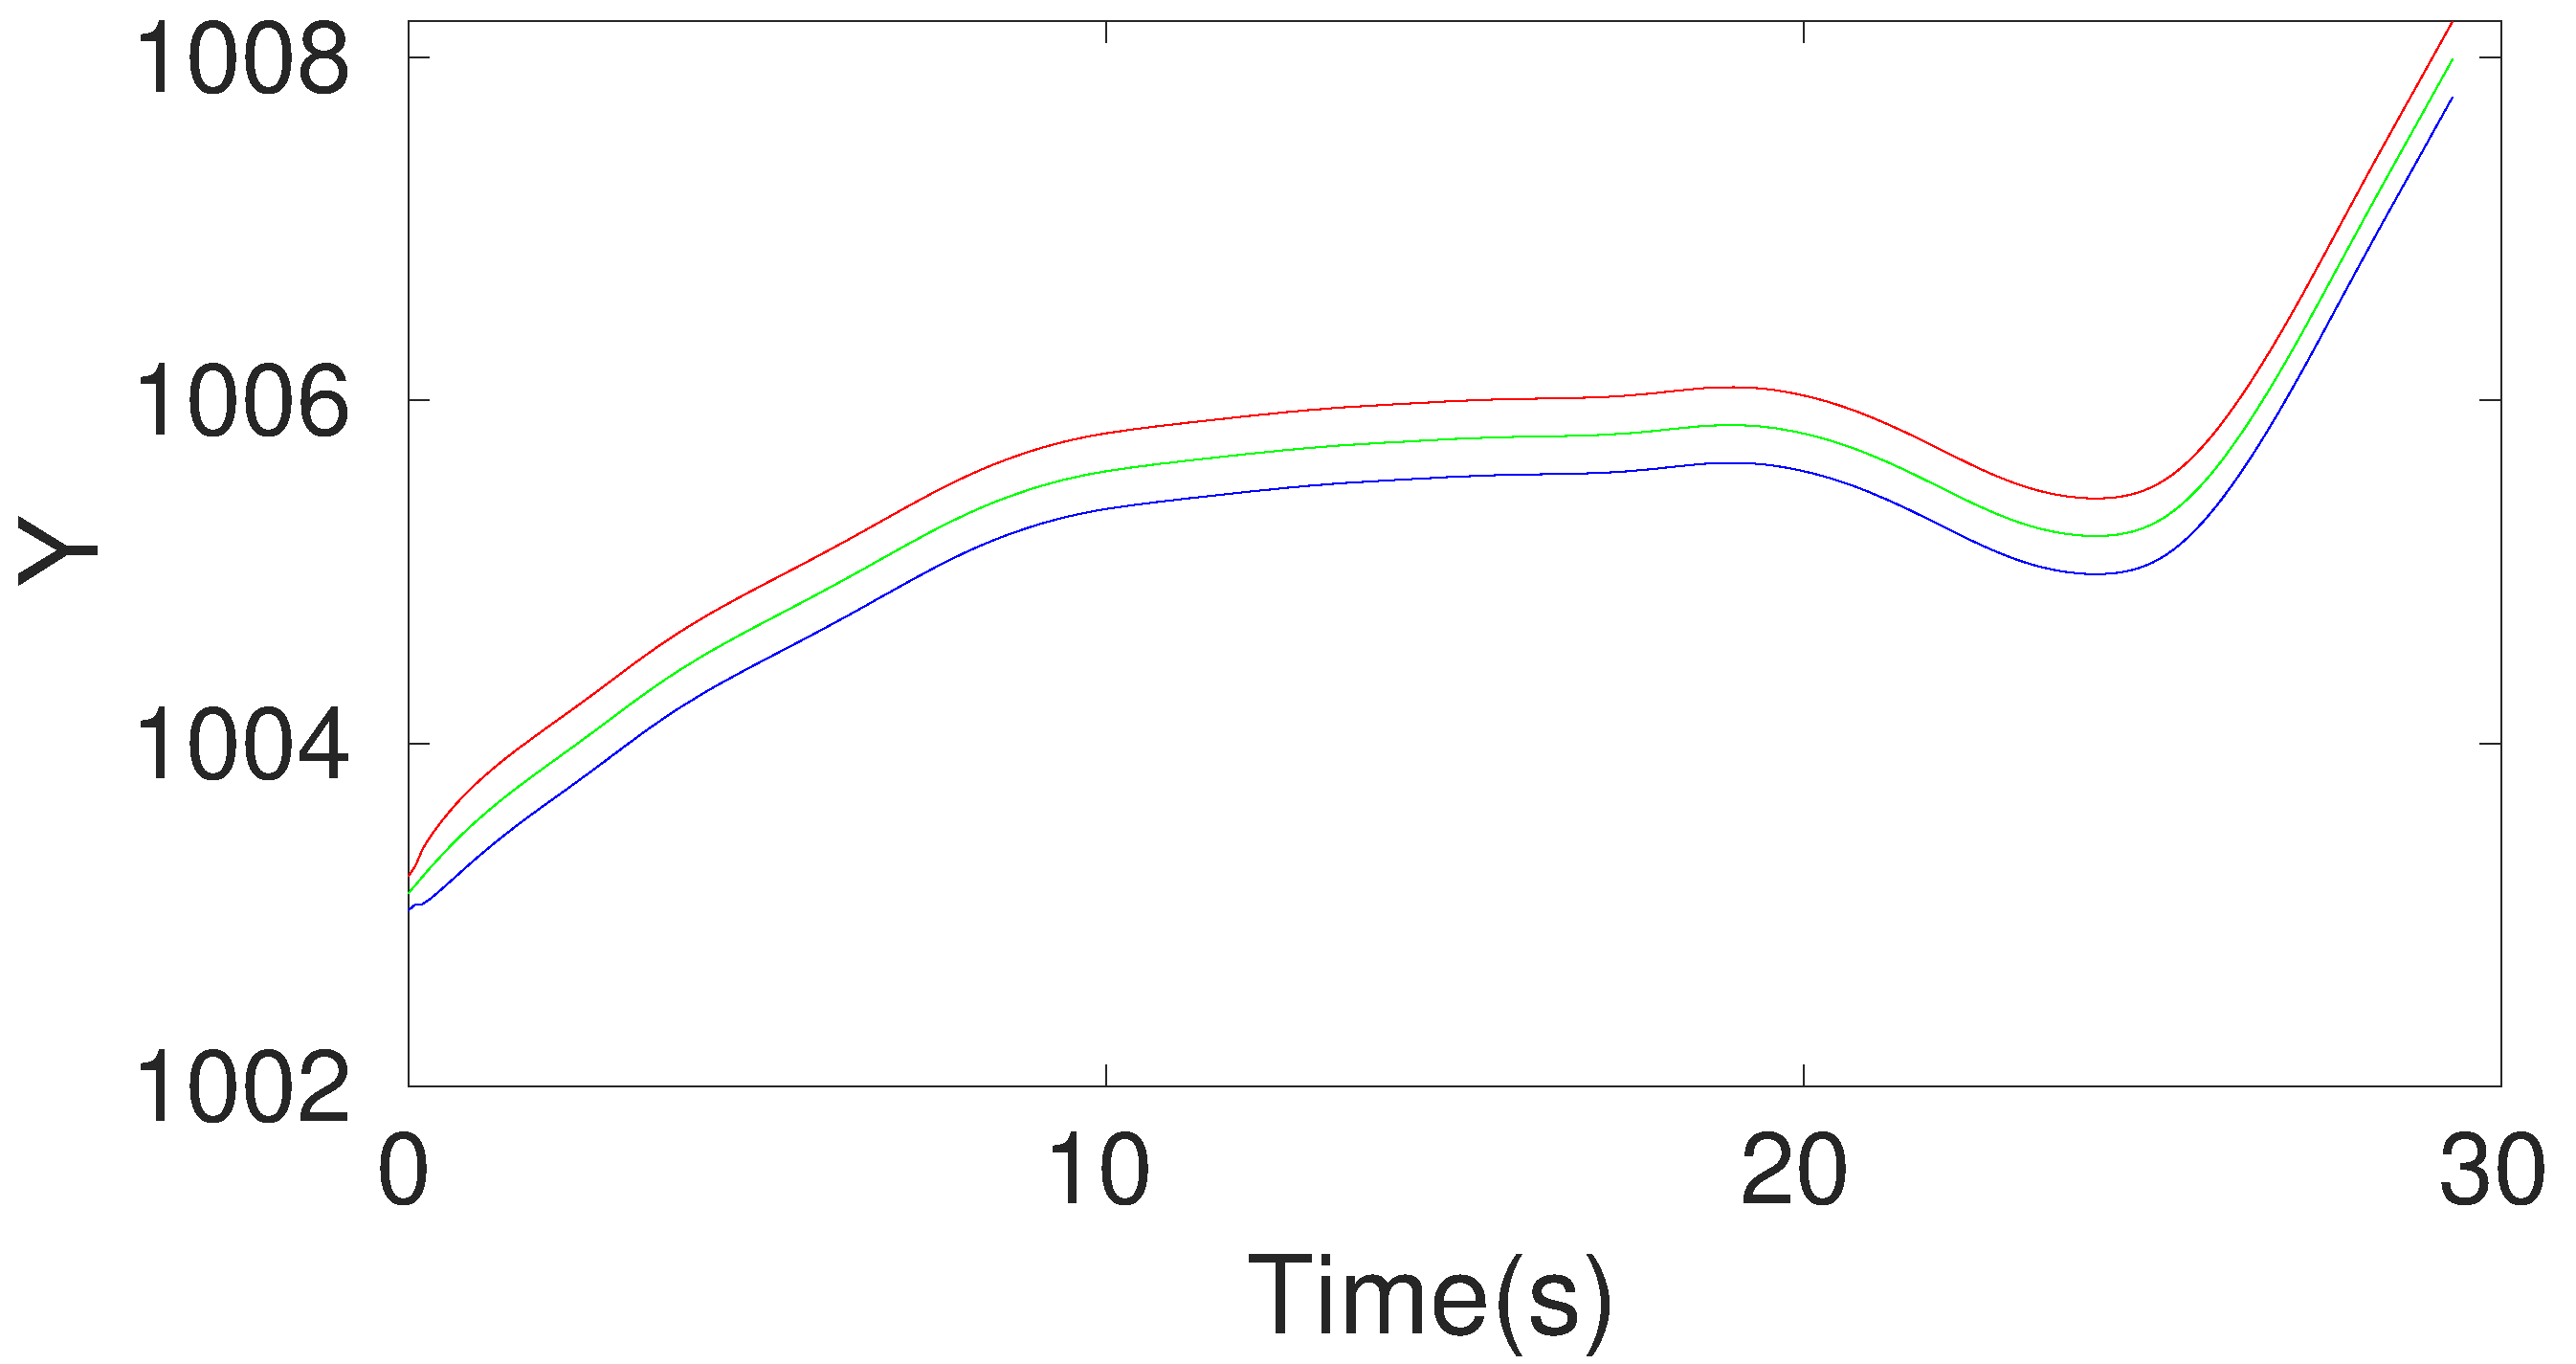
\includegraphics[width=\linewidth]{figures/Frad/s3cvSMY}
\end{subfigure}
\begin{subfigure}{.5\linewidth}
\centering
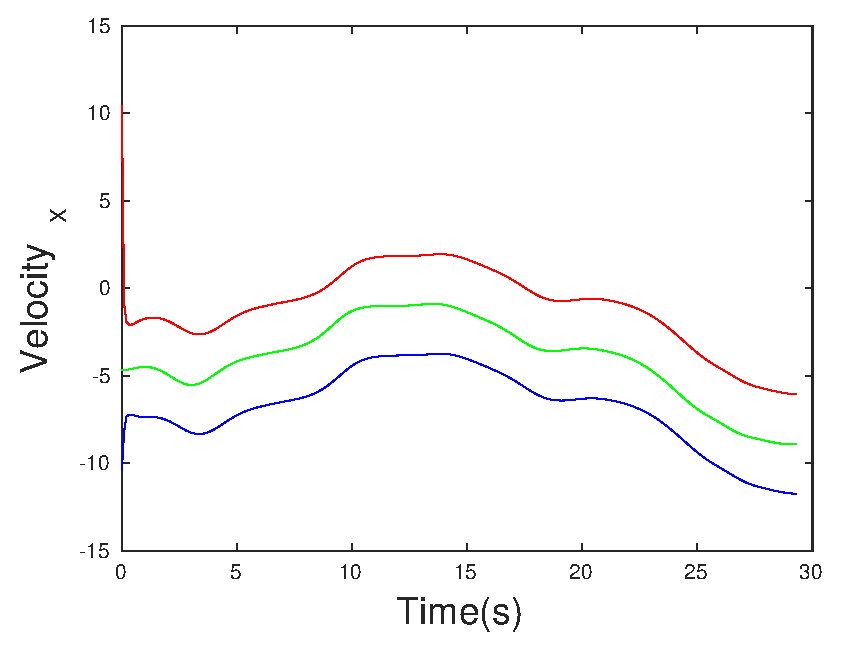
\includegraphics[width=.9\linewidth]{figures/Frad/s3cvSMVelocity_x}
\end{subfigure}
\begin{subfigure}{.5\linewidth}
\centering
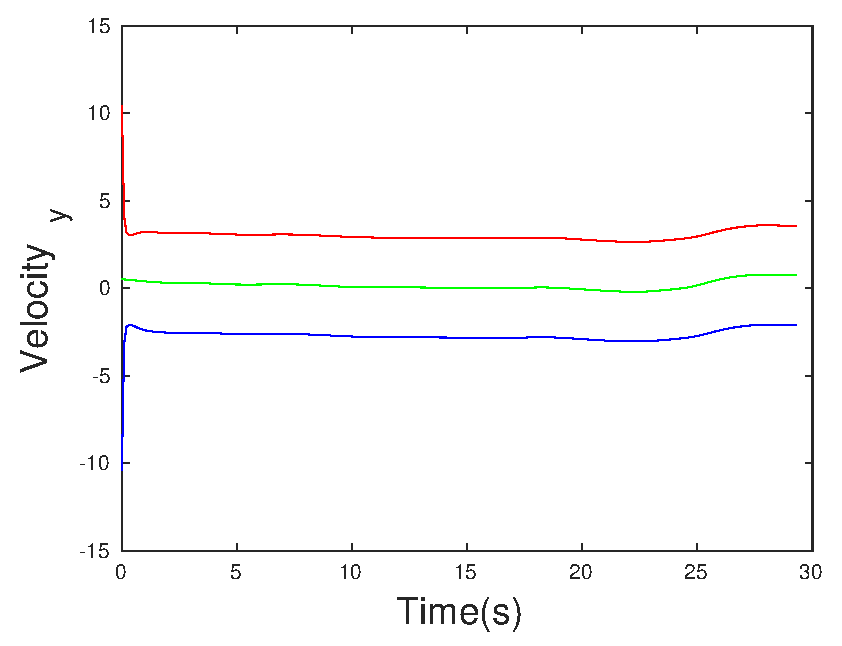
\includegraphics[width=.9\linewidth]{figures/Frad/s3cvSMVelocity_y}
\end{subfigure}
\caption{Estimation using Constant Velocity}
\end{figure}

\begin{figure}[!h]
\begin{subfigure}{.5\linewidth}
\centering
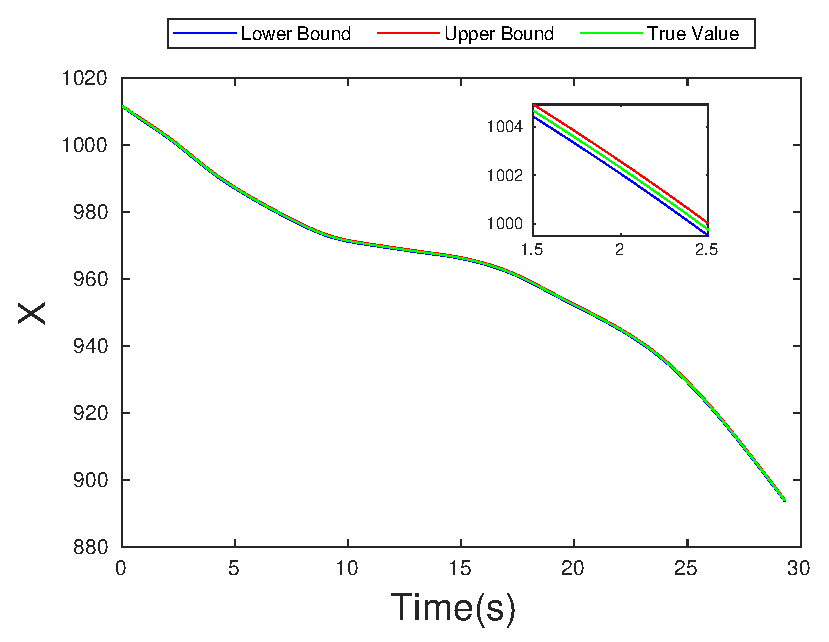
\includegraphics[width=\linewidth]{figures/Frad/s3caSMX}
\end{subfigure}
\begin{subfigure}{.5\linewidth}
\centering
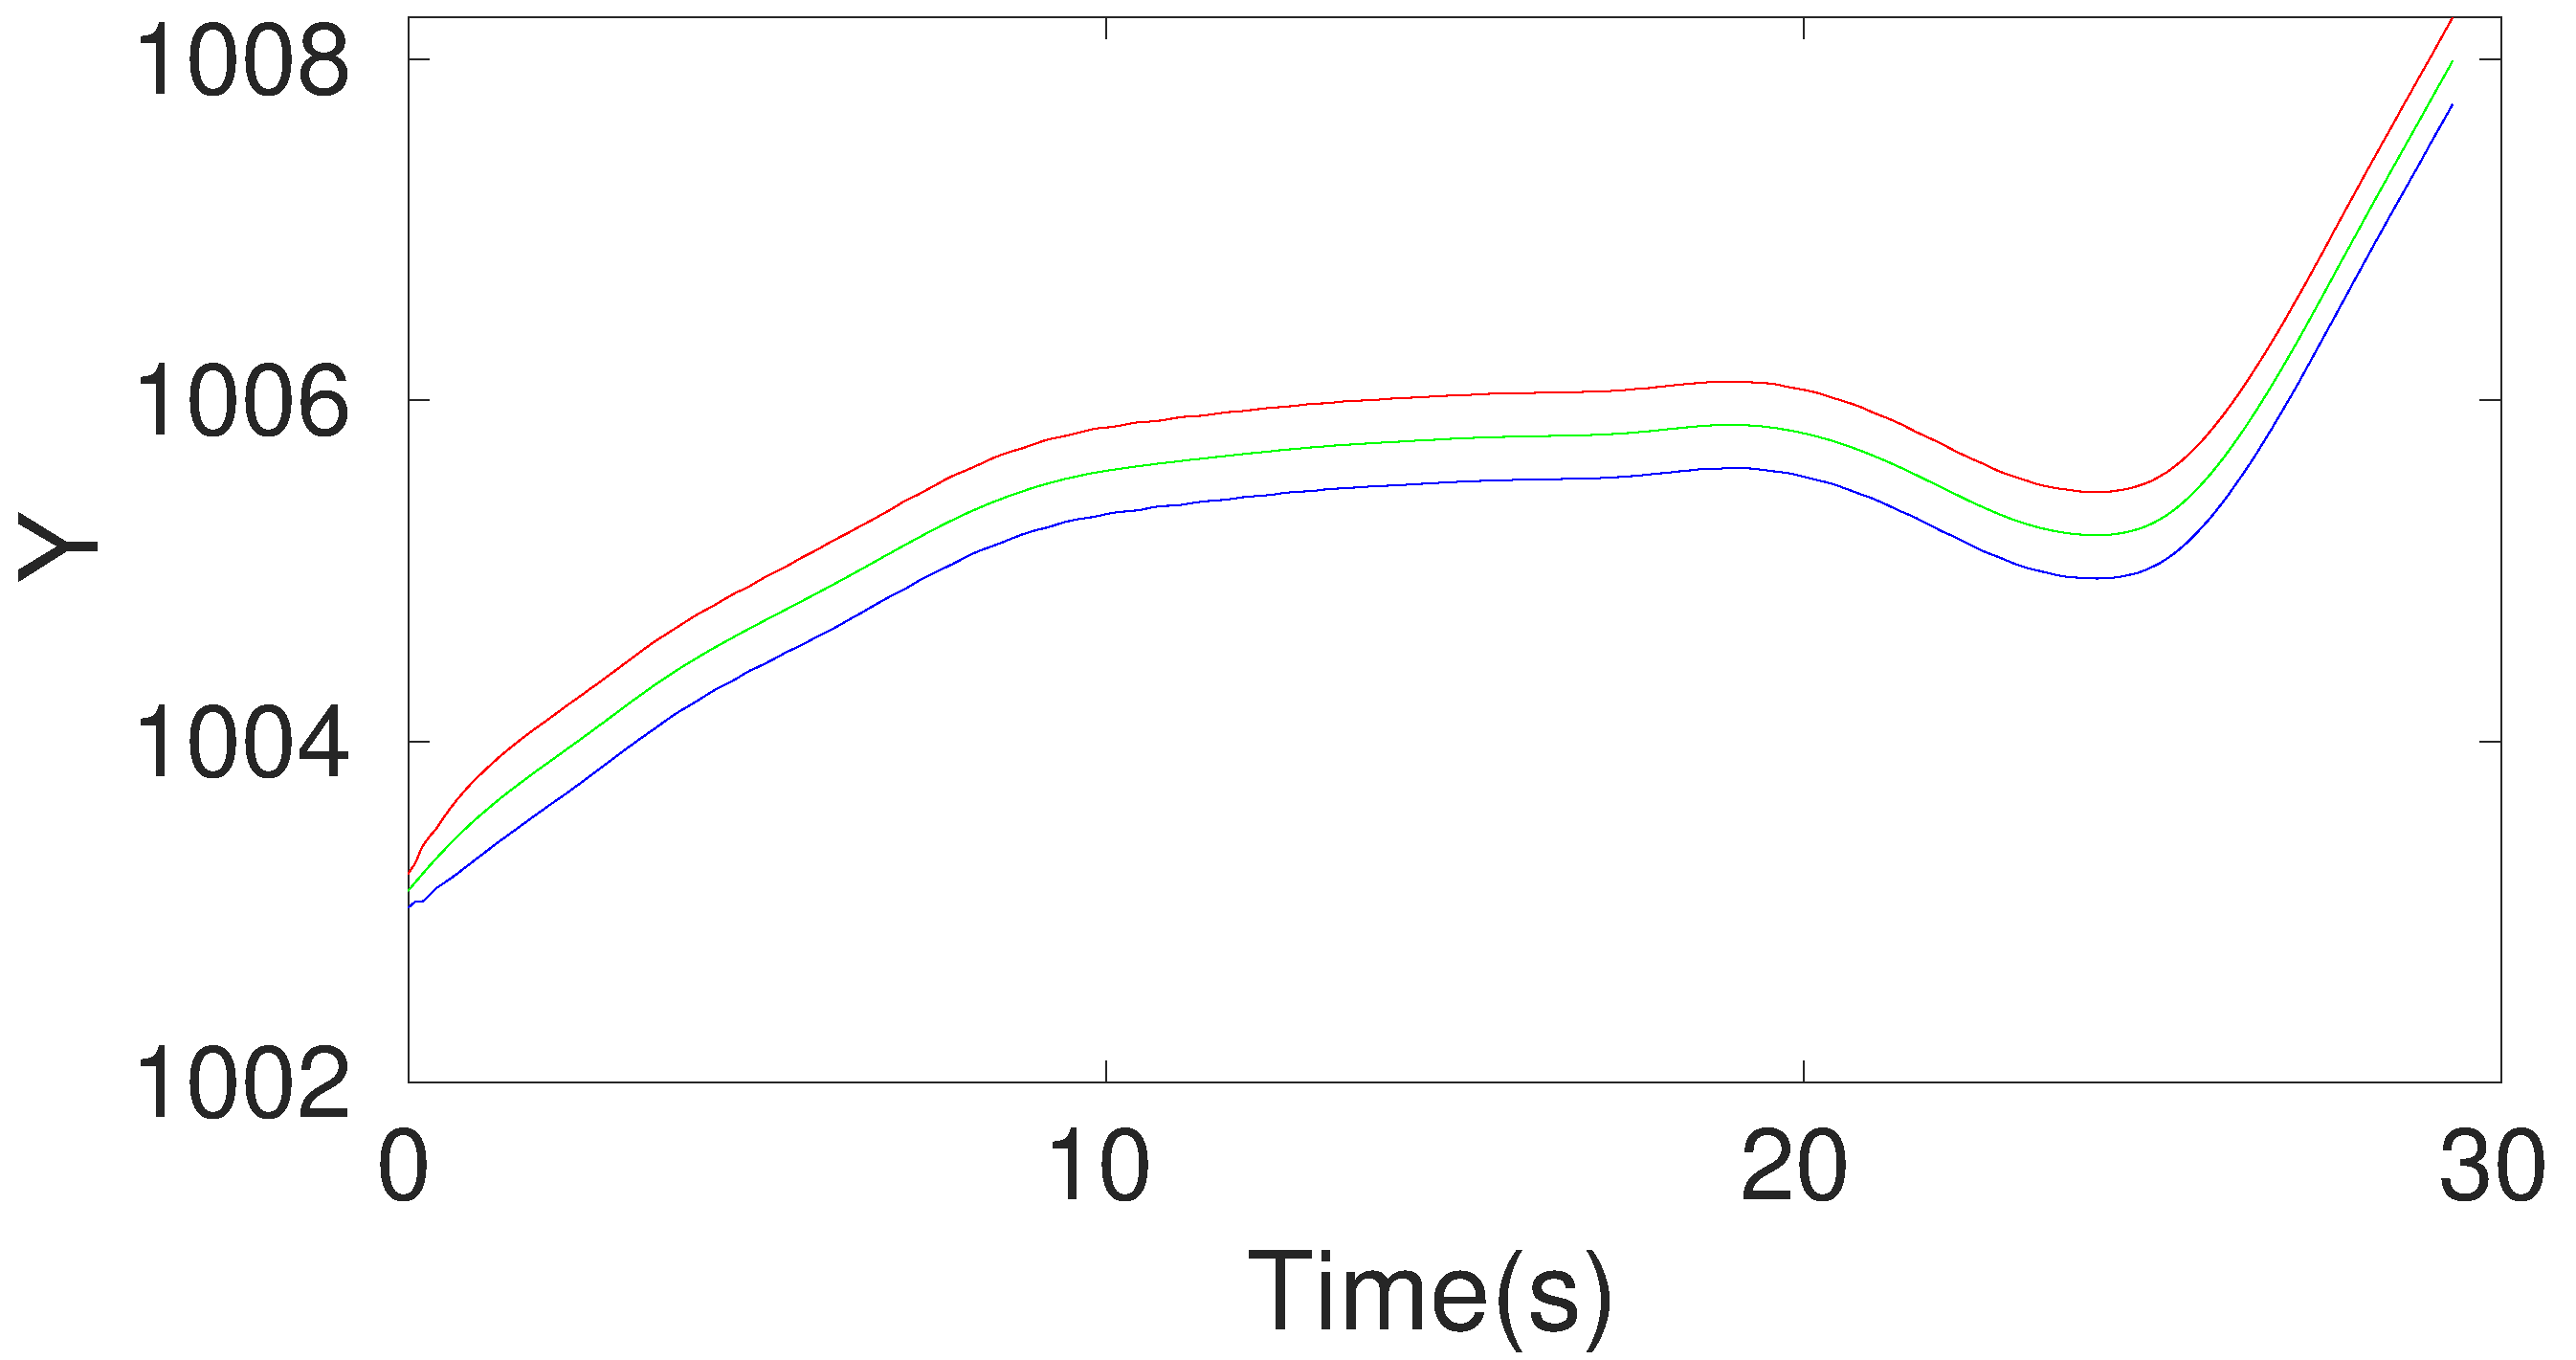
\includegraphics[width=\linewidth]{figures/Frad/s3caSMY}
\end{subfigure}
\begin{subfigure}{.5\linewidth}
\centering
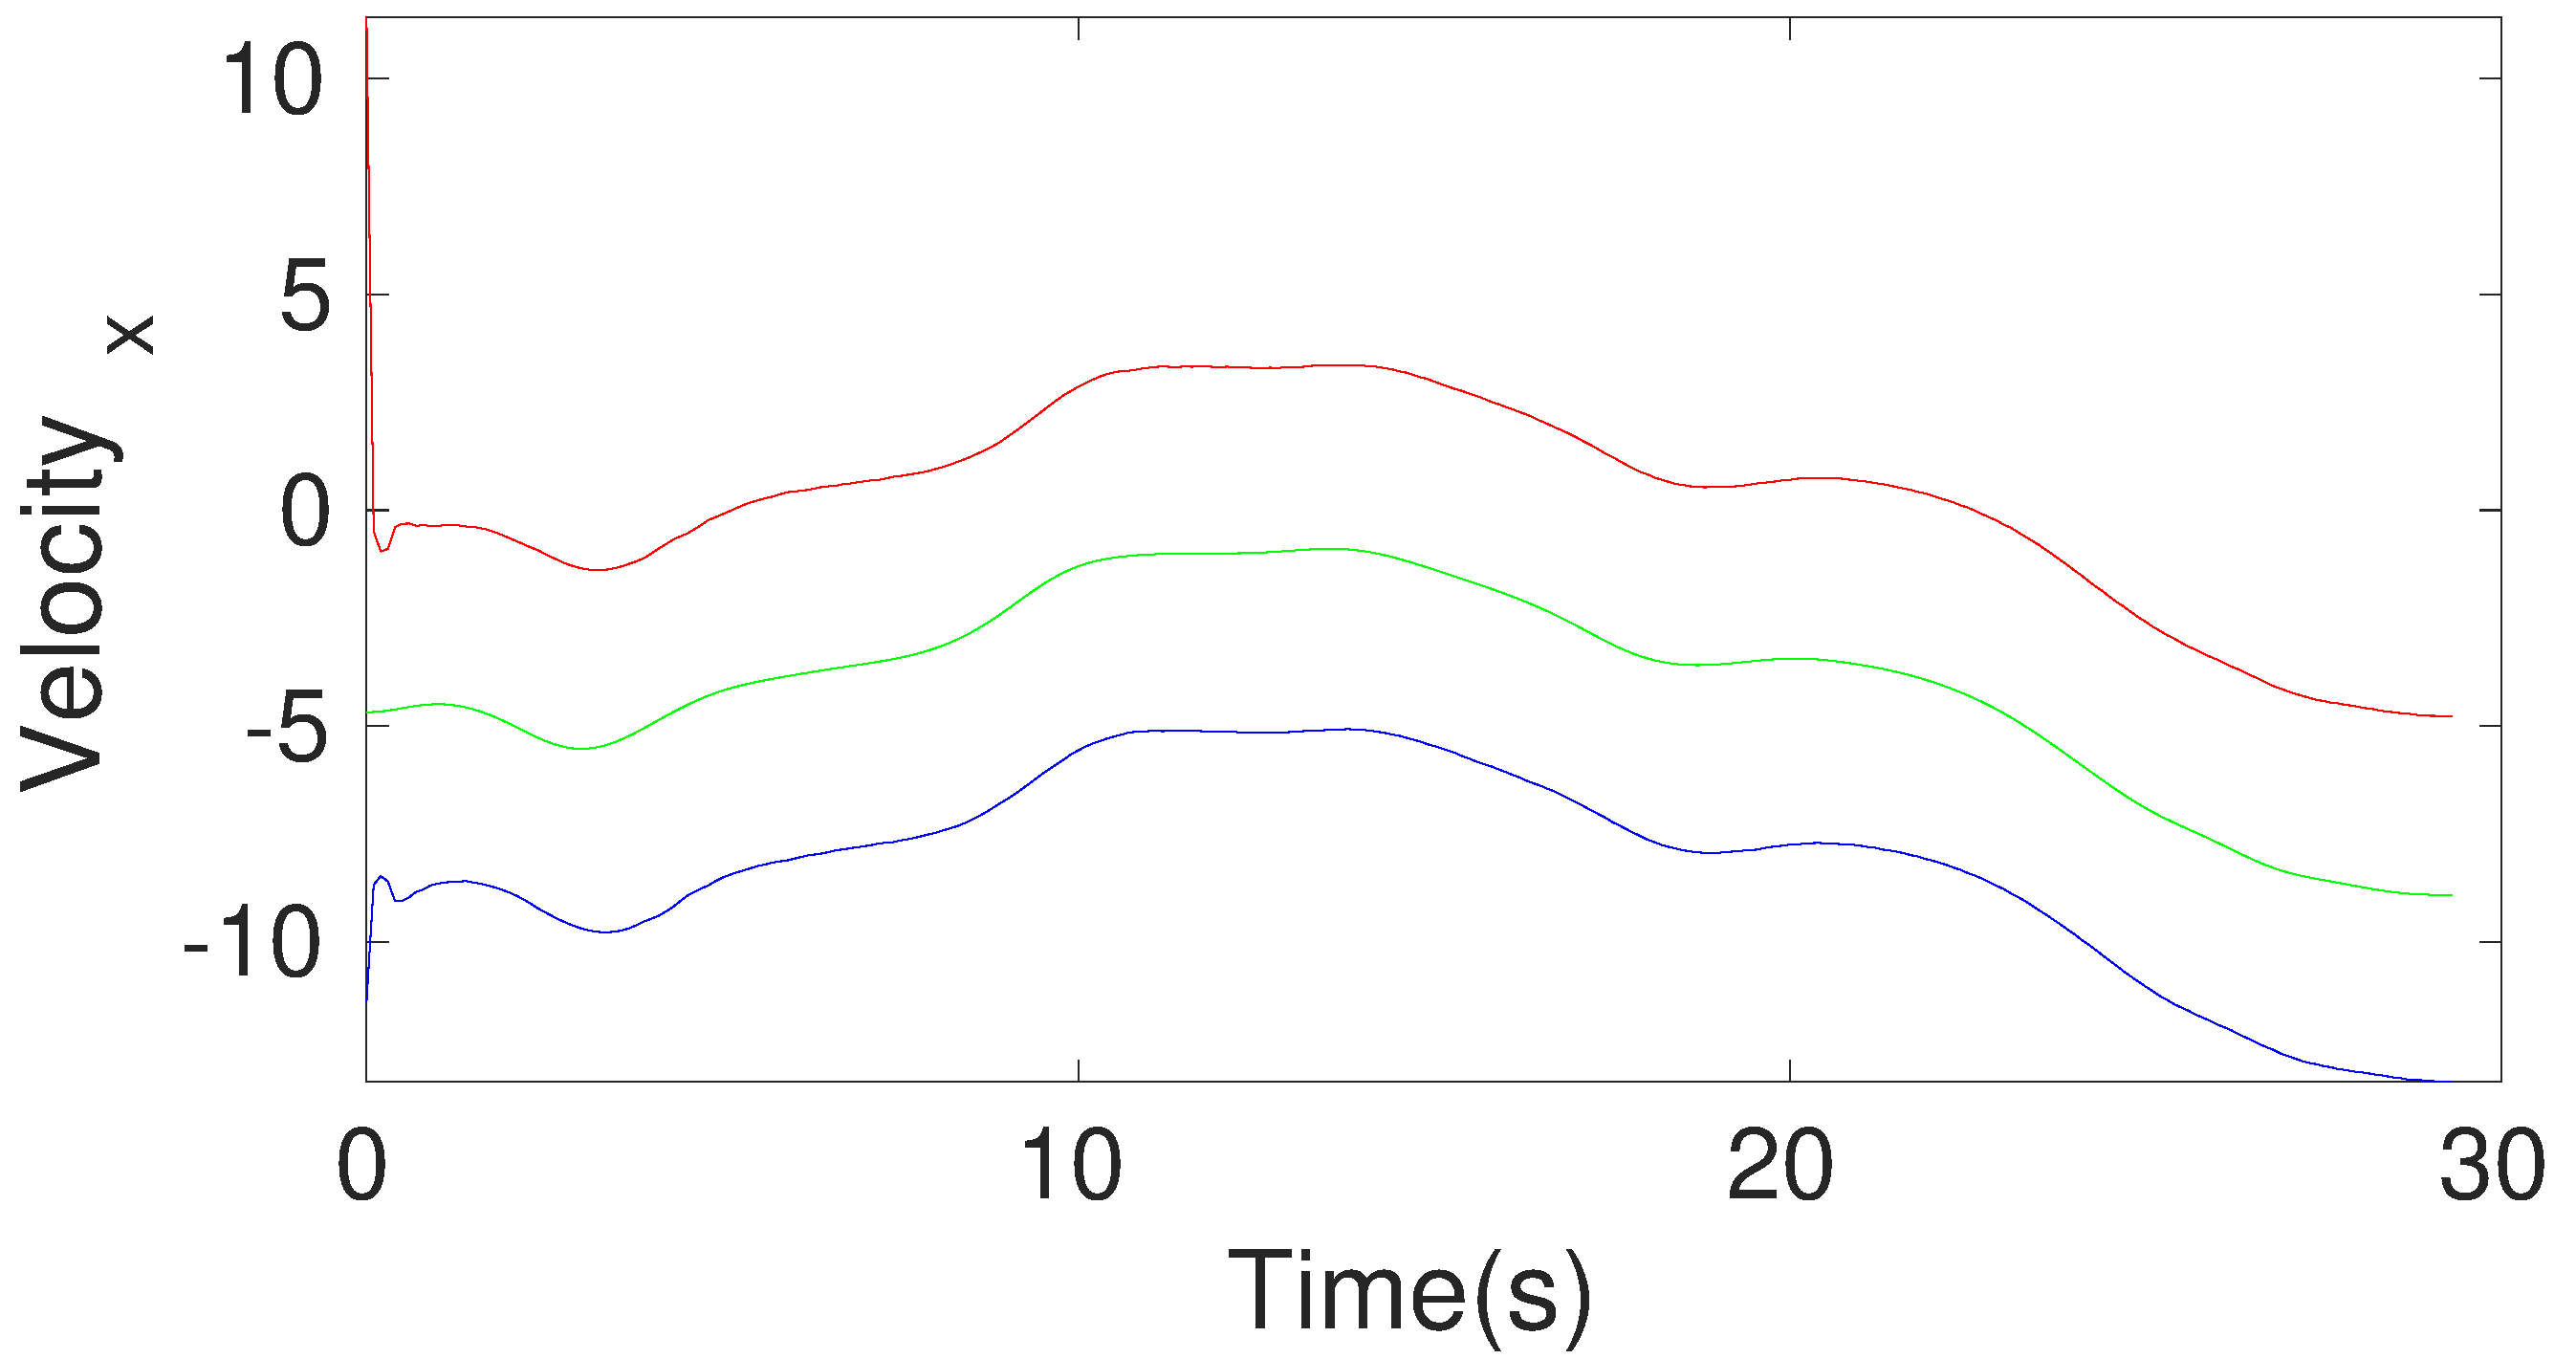
\includegraphics[width=.9\linewidth]{figures/Frad/s3caSMVelocity_x}
\end{subfigure}
\begin{subfigure}{.5\linewidth}
\centering
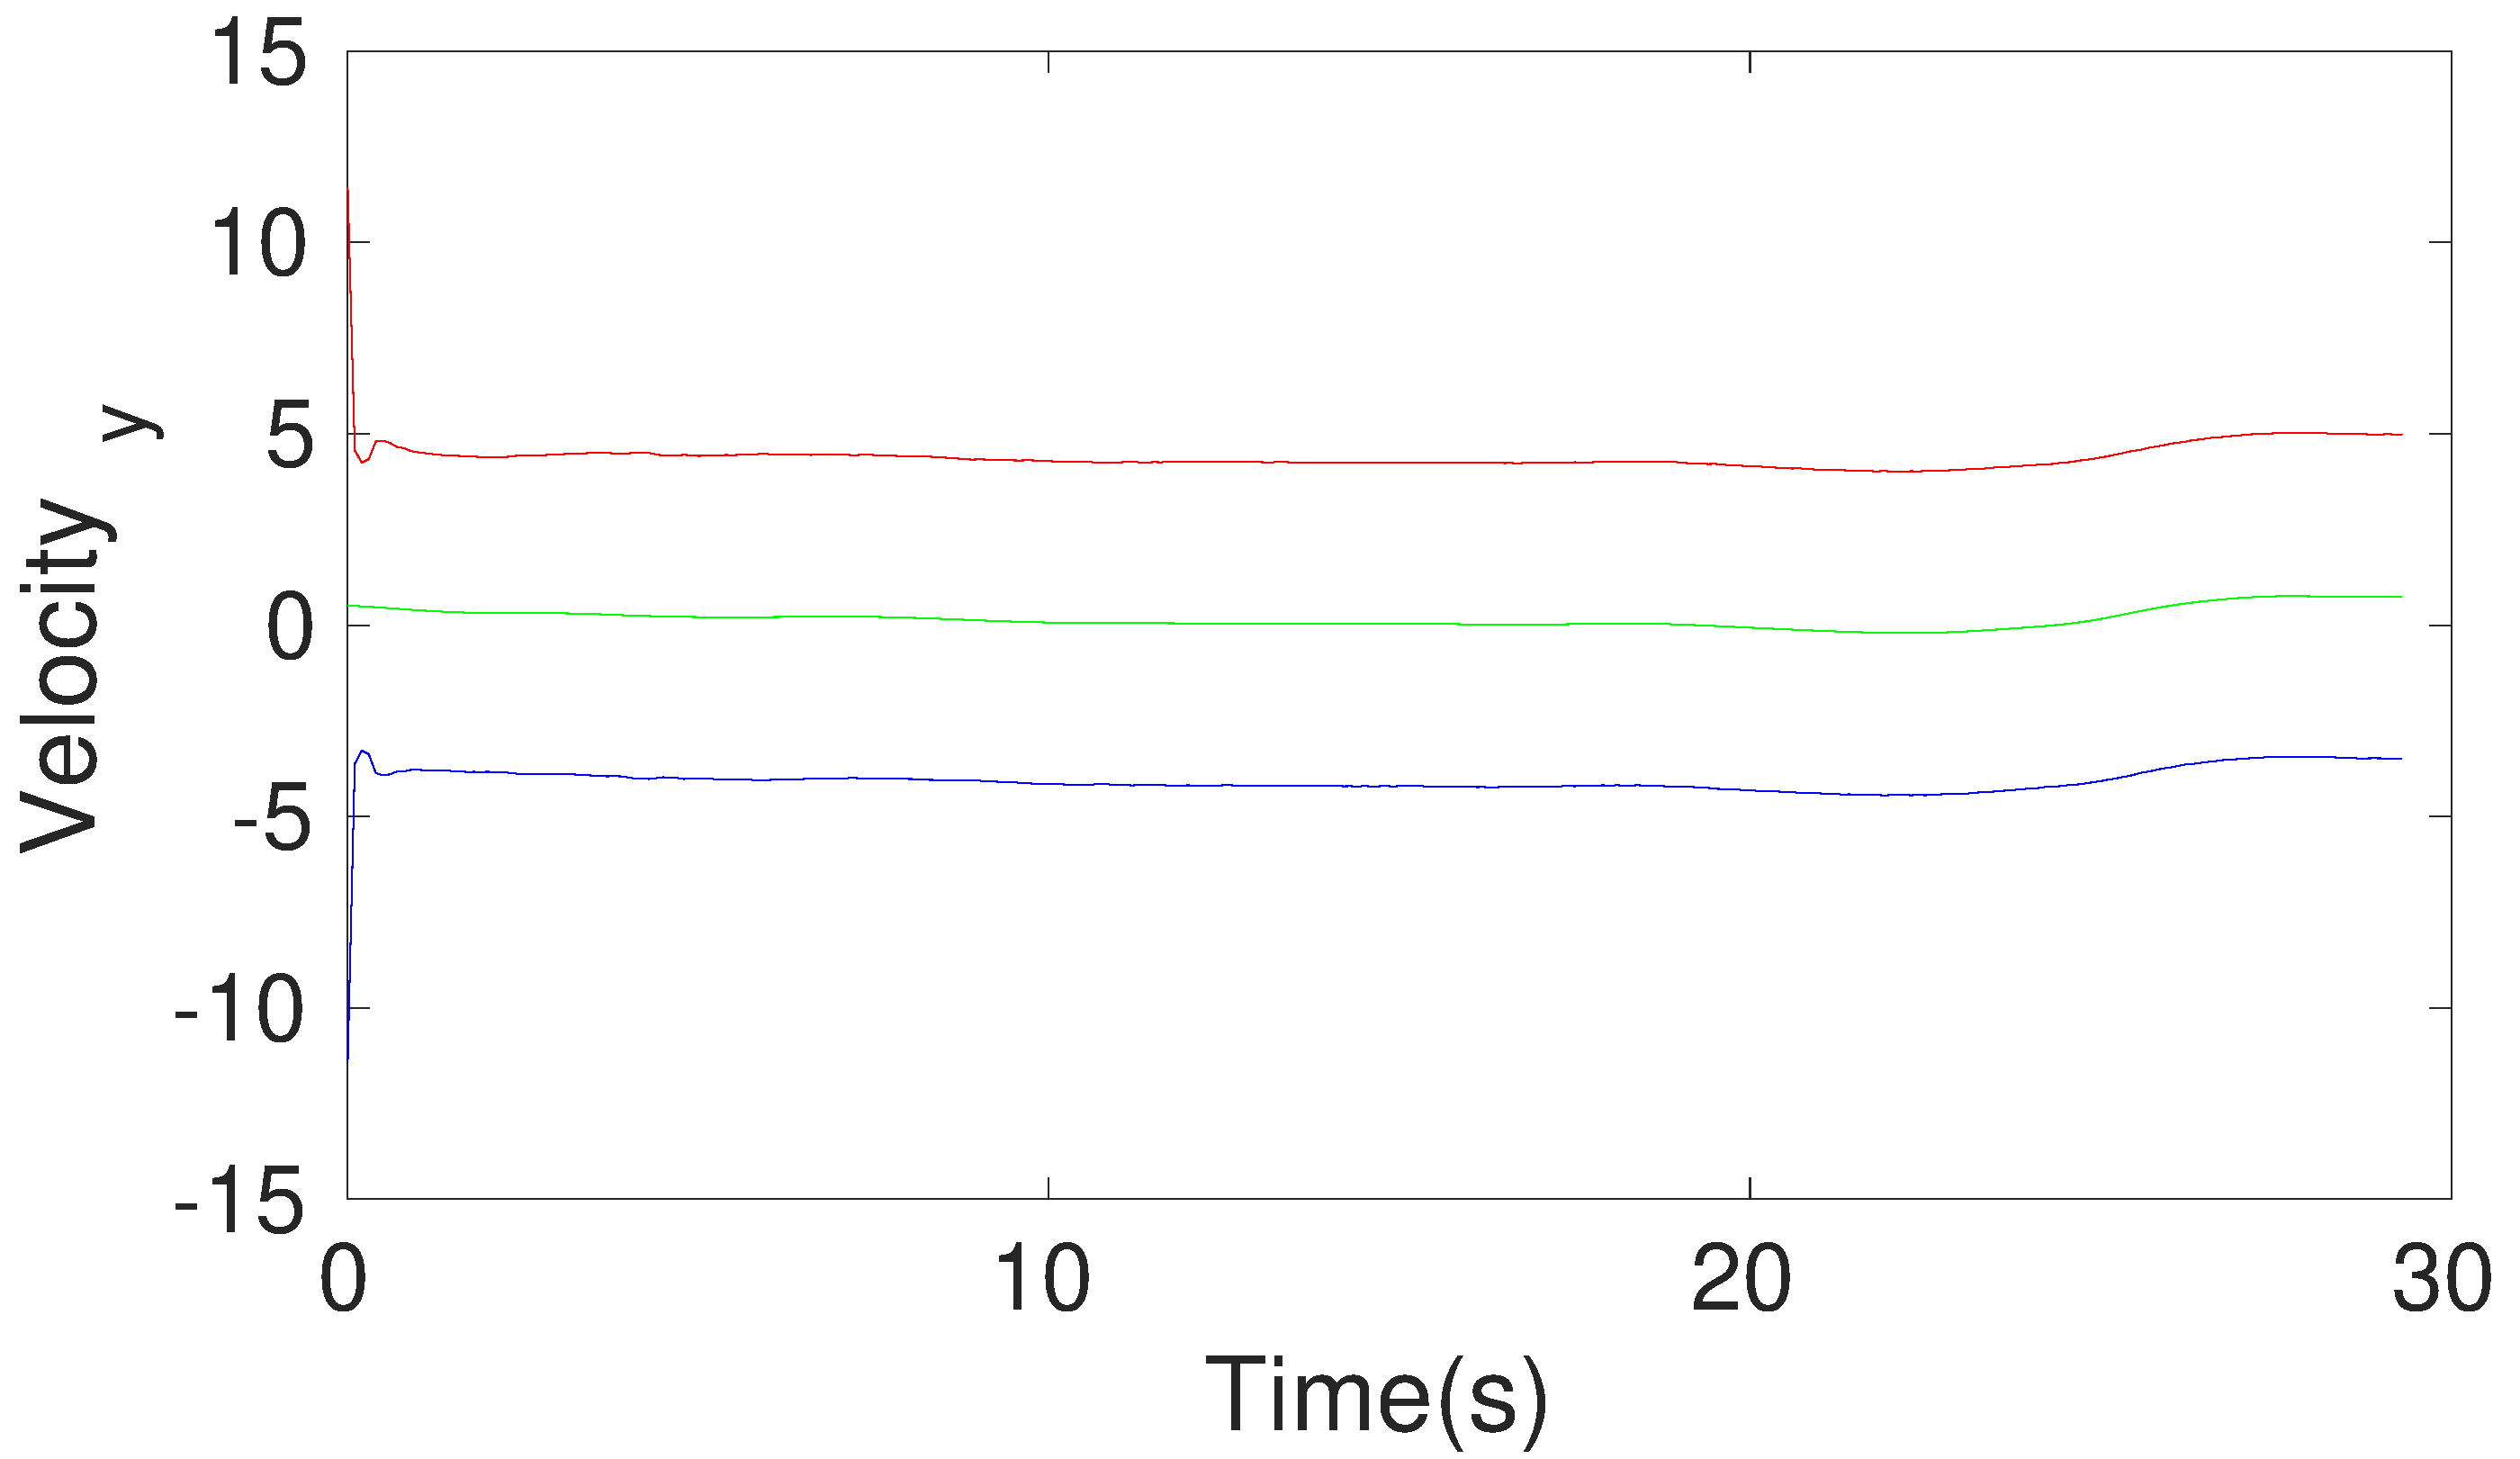
\includegraphics[width=.9\linewidth]{figures/Frad/s3caSMVelocity_y}
\end{subfigure}
\begin{subfigure}{.5\linewidth}
\centering
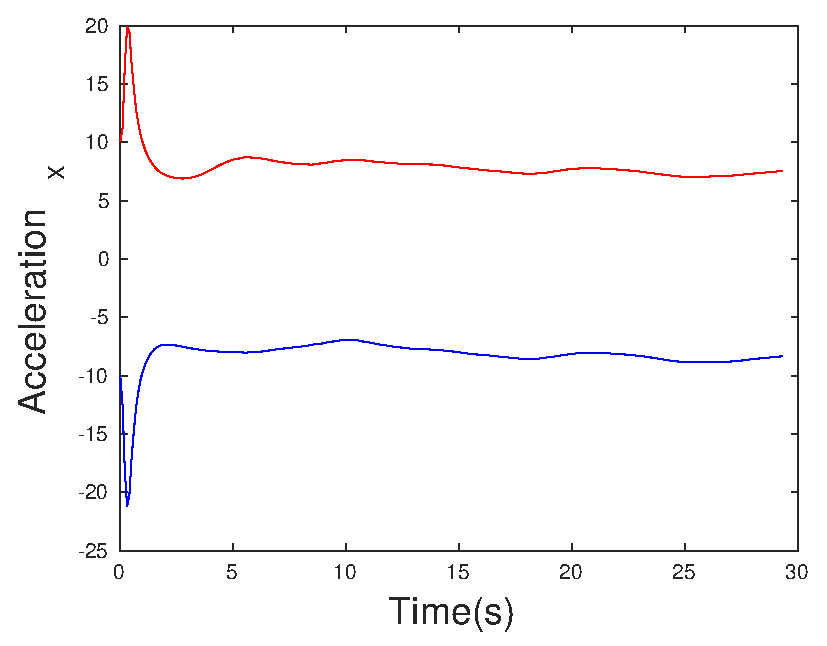
\includegraphics[width=.9\linewidth]{figures/Frad/s3caSMAcceleration_x}
\end{subfigure}
\begin{subfigure}{.5\linewidth}
\centering
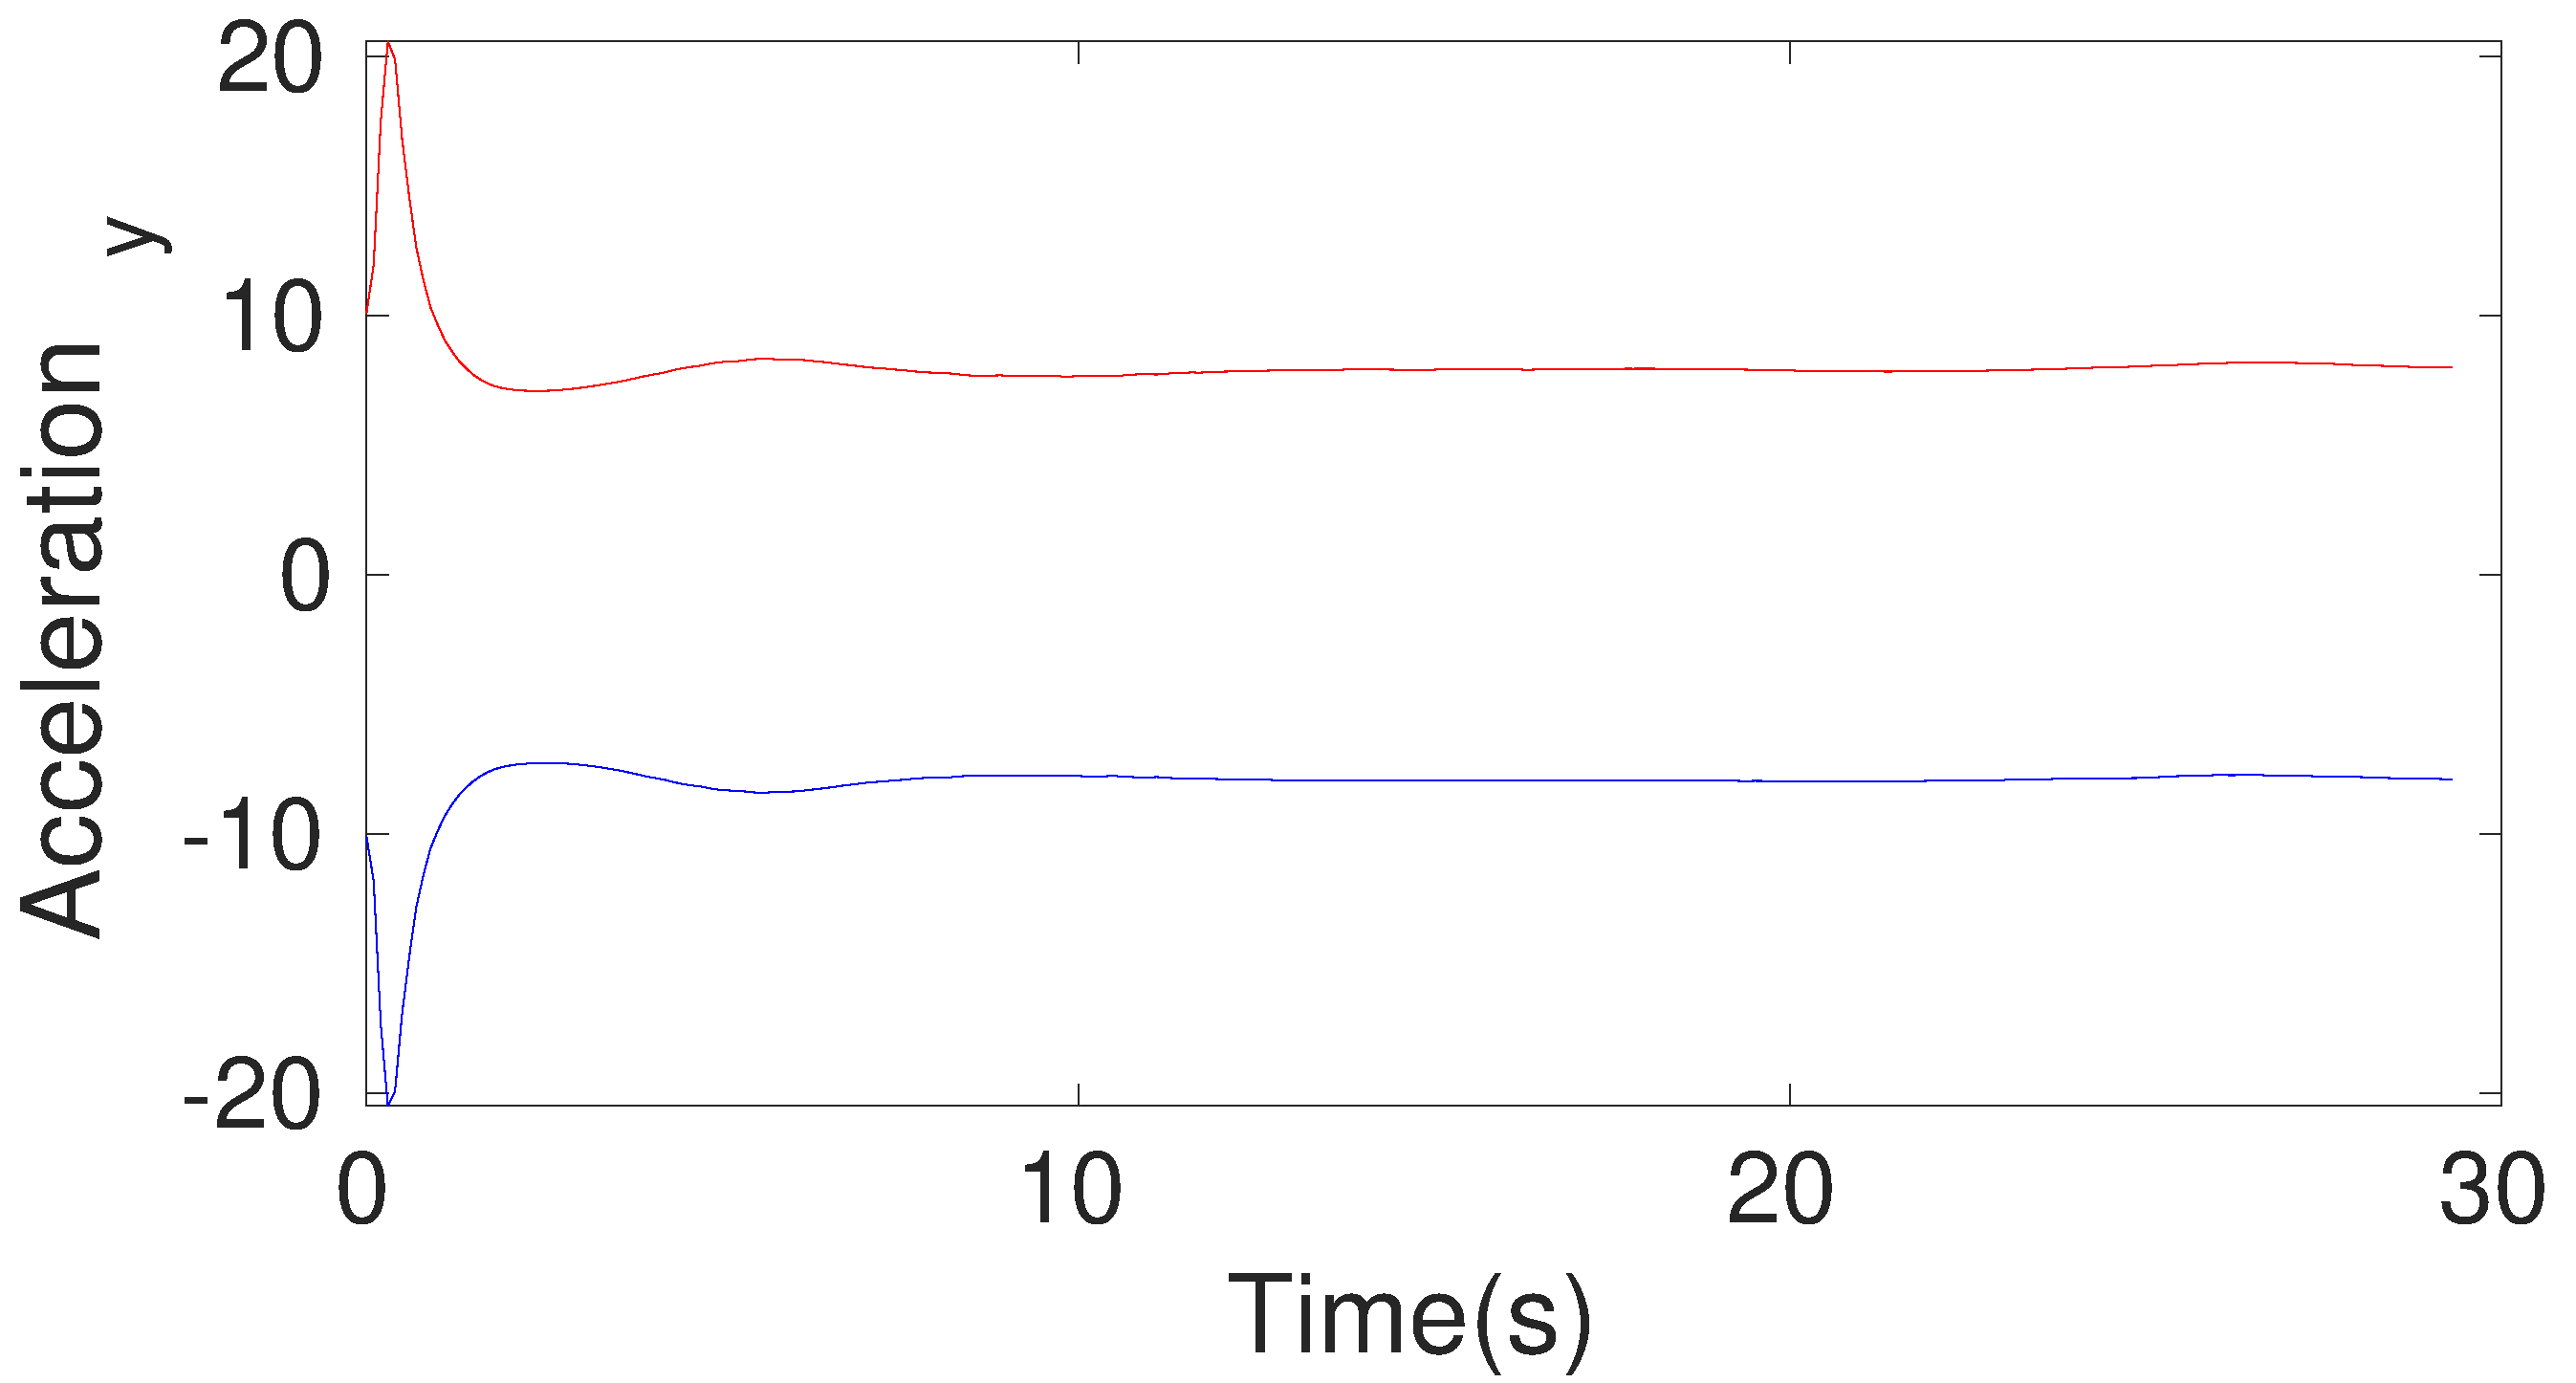
\includegraphics[width=.9\linewidth]{figures/Frad/s3caSMAcceleration_y}
\end{subfigure}
\caption{Estimation using Constant Acceleration}
\end{figure}

\begin{figure}[h]
\begin{subfigure}{.5\linewidth}
\centering
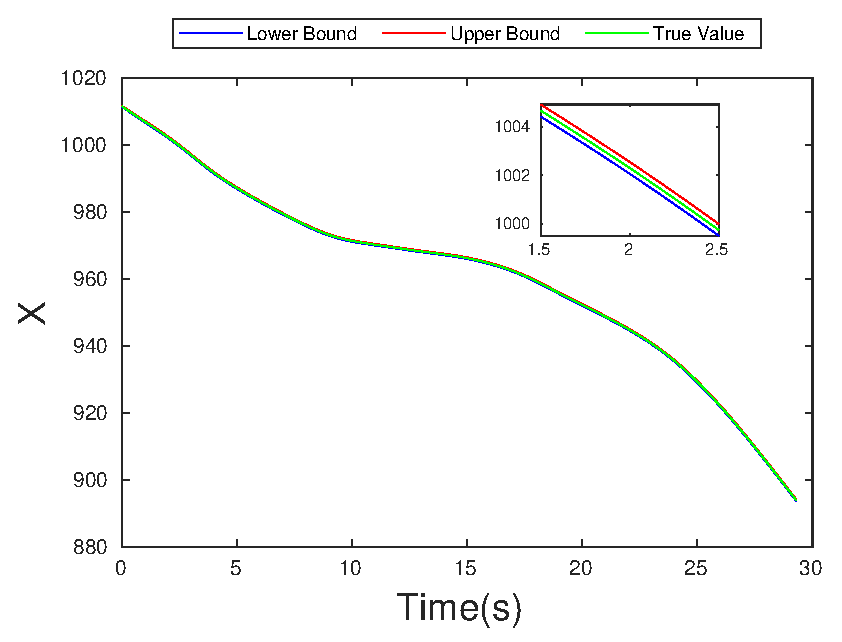
\includegraphics[width=\linewidth]{figures/Frad/s3csSMX}
\end{subfigure}
\begin{subfigure}{.5\linewidth}
\centering
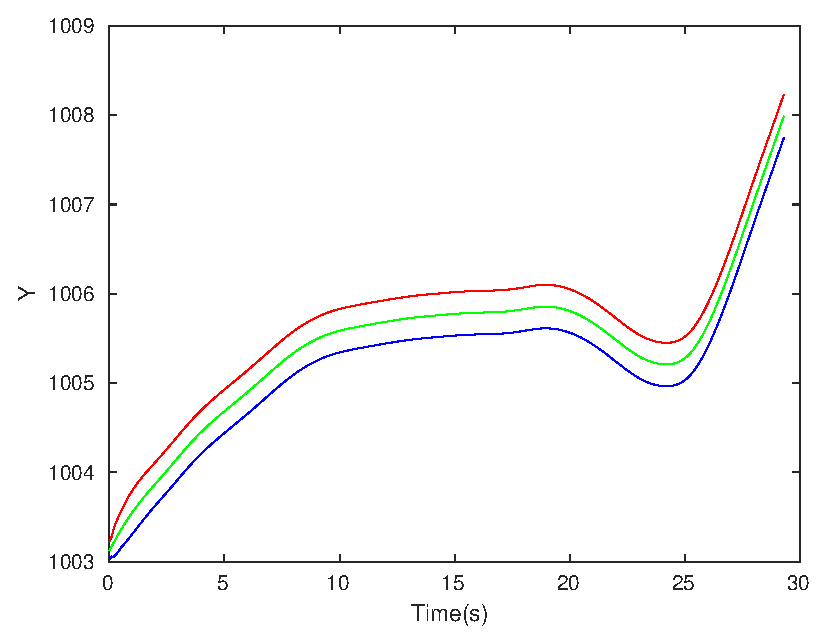
\includegraphics[width=\linewidth]{figures/Frad/s3csSMY}
\end{subfigure}
\begin{subfigure}{.5\linewidth}
\centering
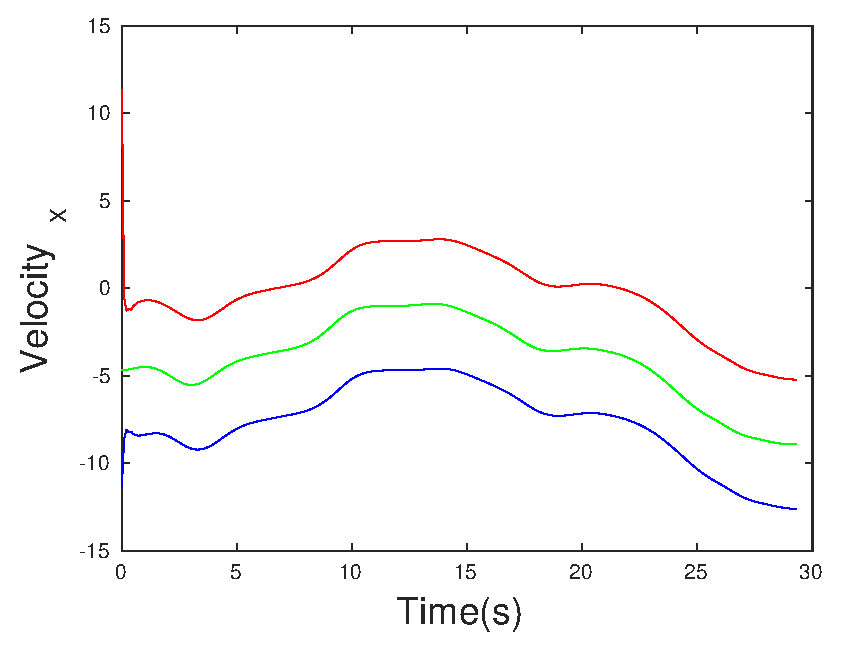
\includegraphics[width=.9\linewidth]{figures/Frad/s3csSMVelocity_x}
\end{subfigure}
\begin{subfigure}{.5\linewidth}
\centering
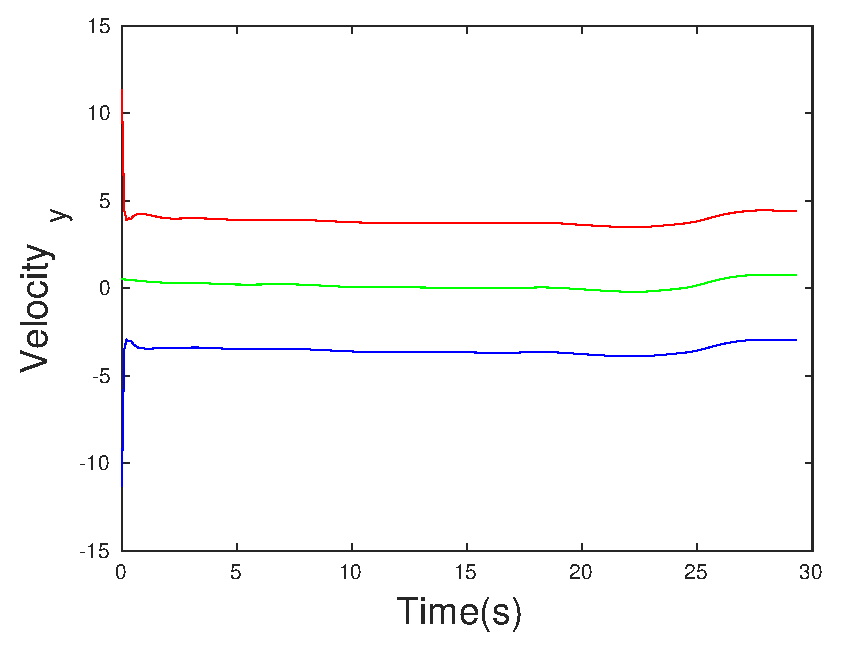
\includegraphics[width=.9\linewidth]{figures/Frad/s3csSMVelocity_y}
\end{subfigure}
\begin{subfigure}{.5\linewidth}
\centering
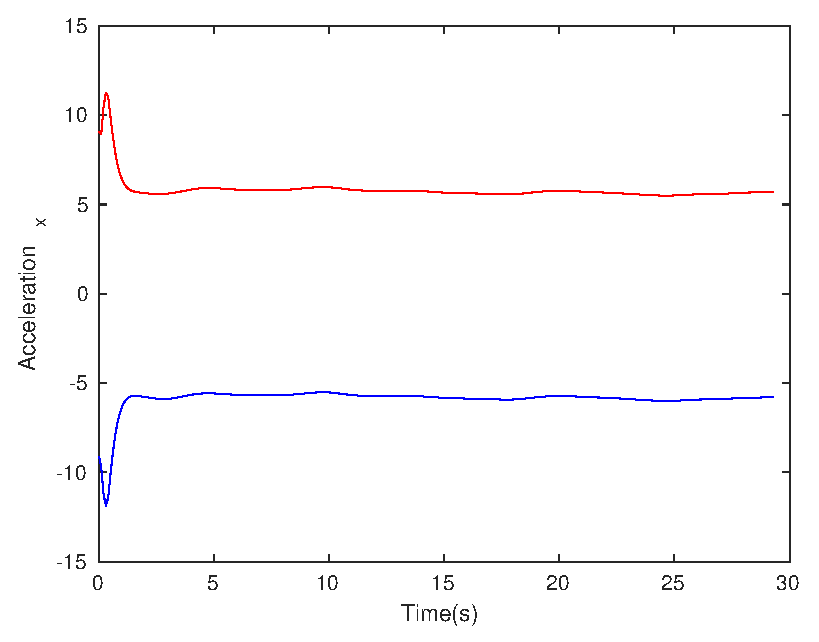
\includegraphics[width=.9\linewidth]{figures/Frad/s3csSMAcceleration_x}
\end{subfigure}
\begin{subfigure}{.5\linewidth}
\centering
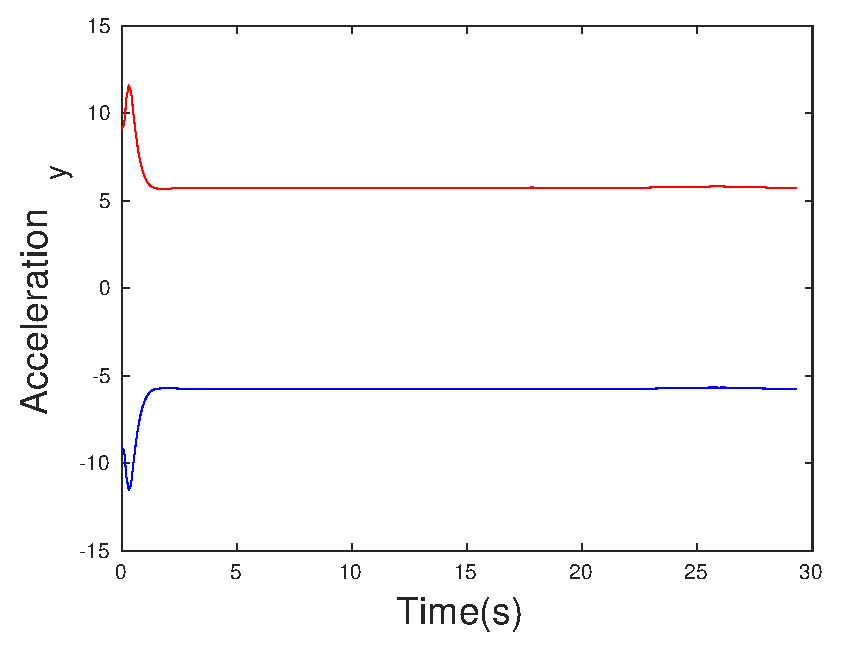
\includegraphics[width=.9\linewidth]{figures/Frad/s3csSMAcceleration_y}
\end{subfigure}
\caption{Estimation using Singer Acceleration}
\end{figure}


\subsection{Segment Minimization using P-Radius}
\begin{figure}[h]
\begin{subfigure}{.5\linewidth}
\centering
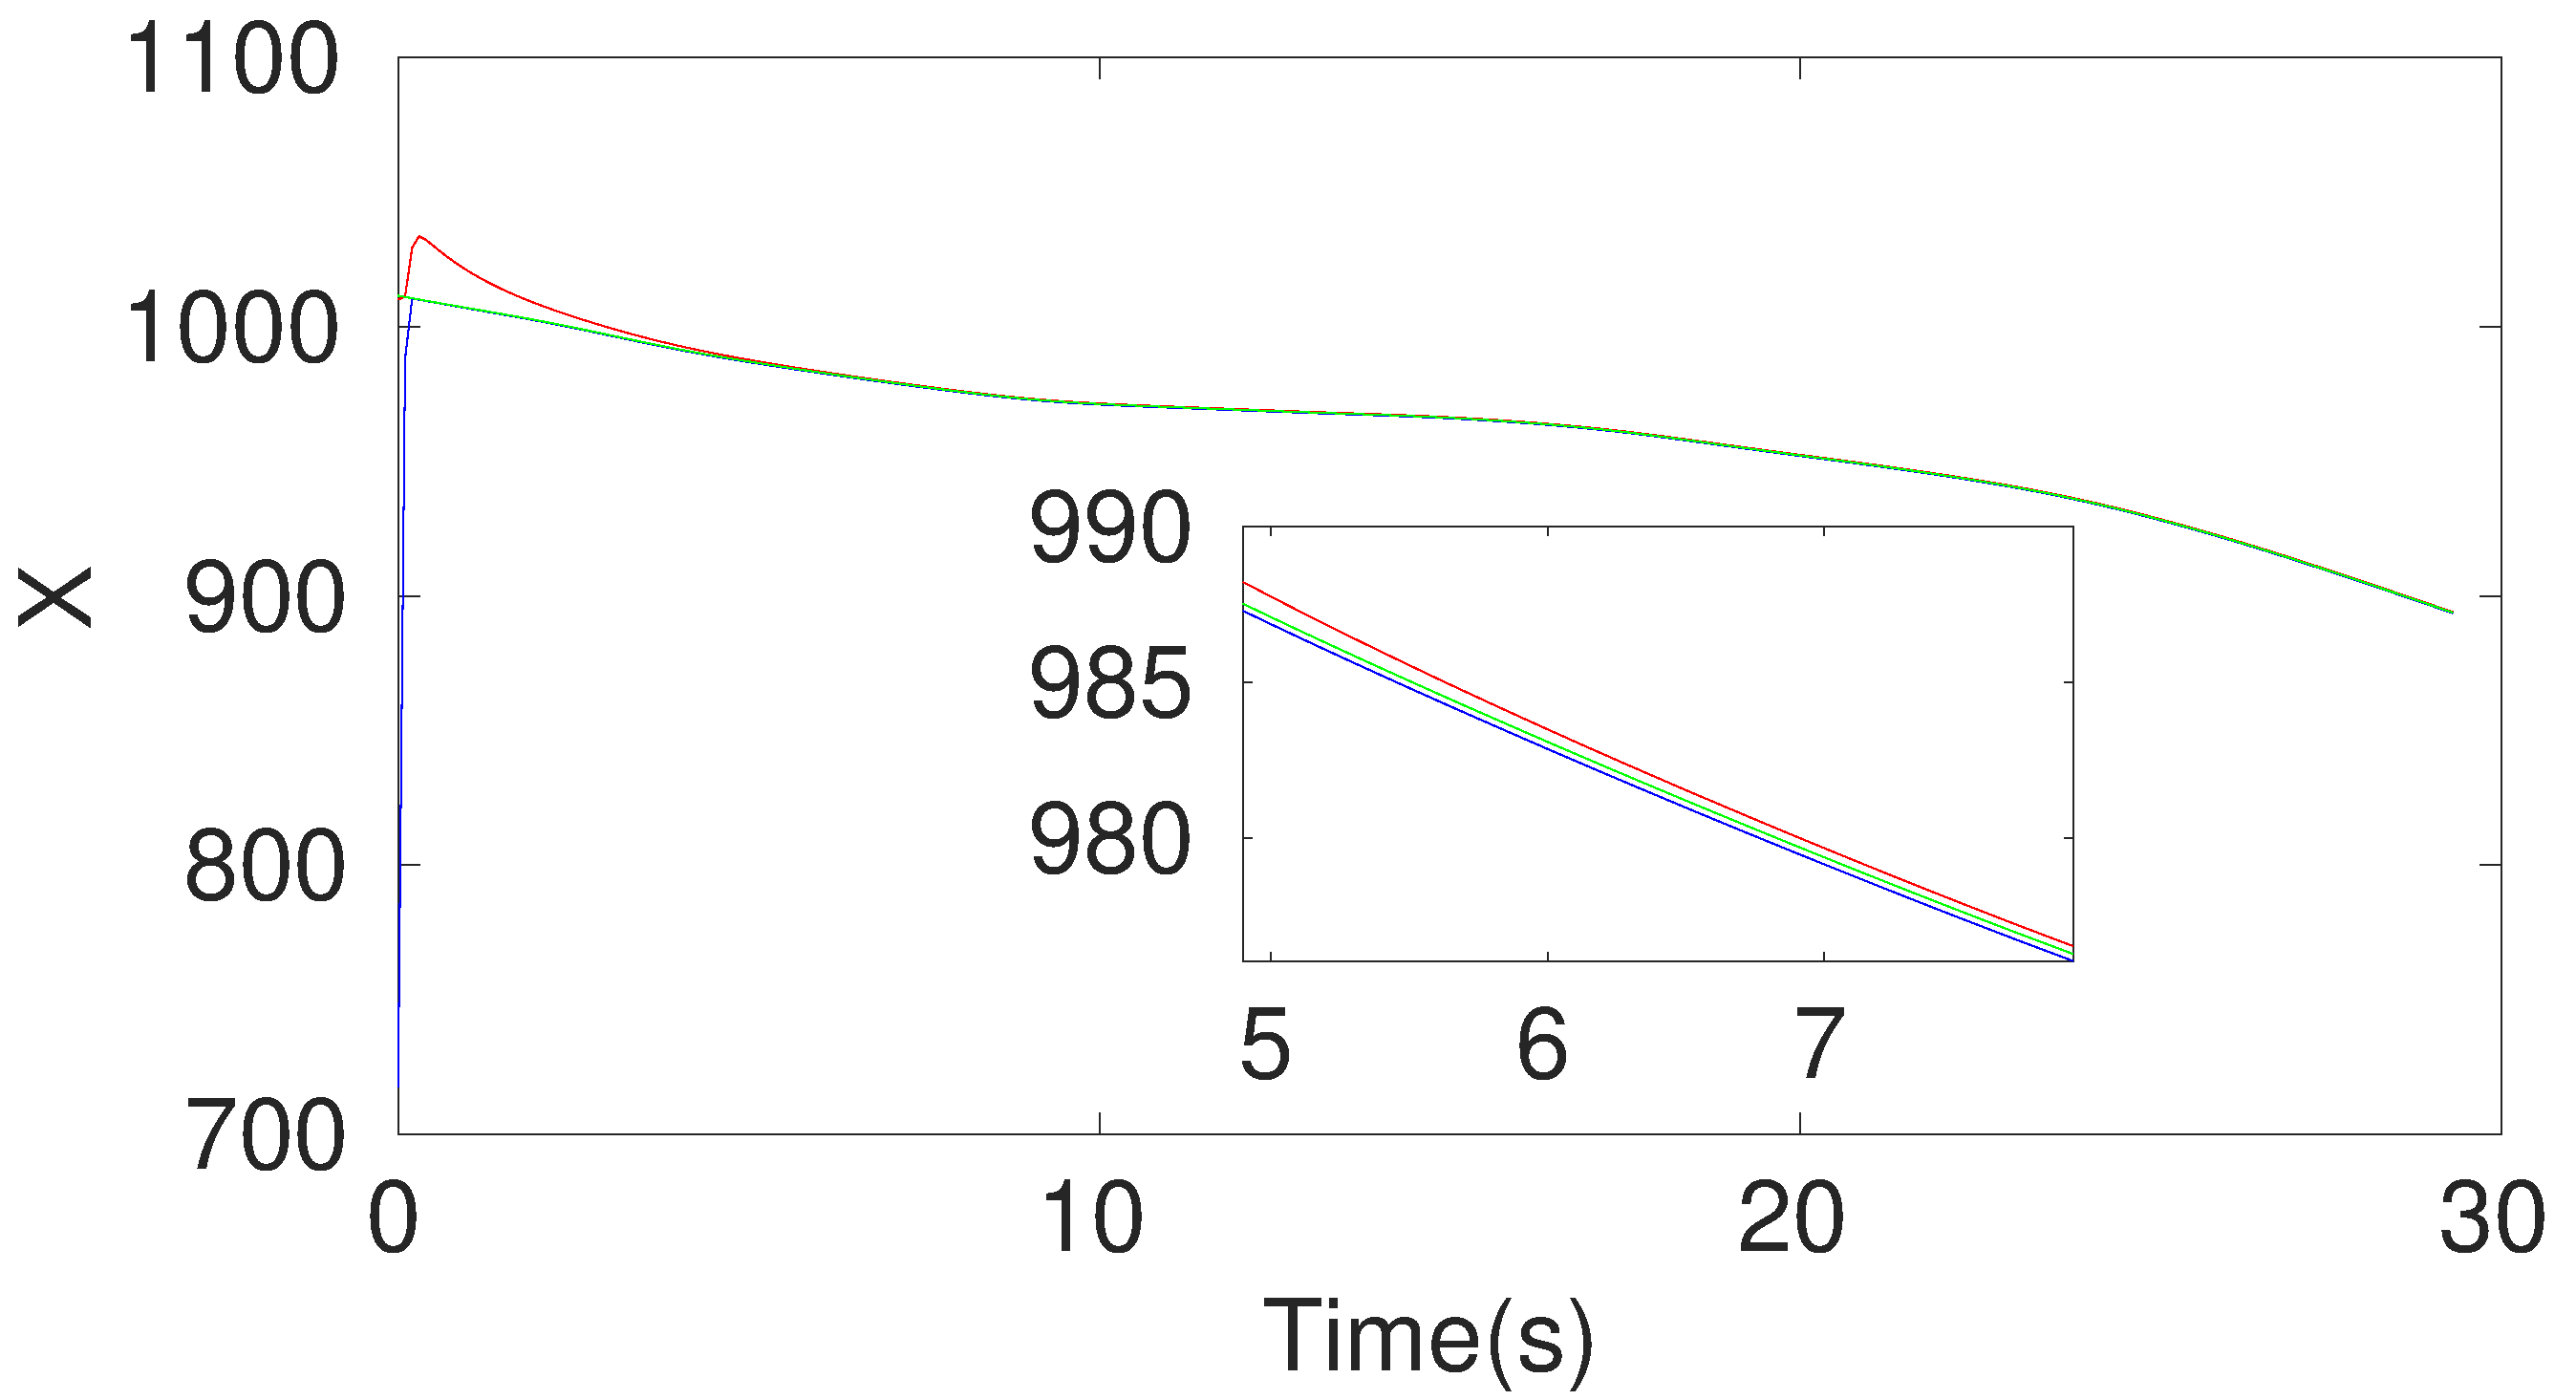
\includegraphics[width=\linewidth]{figures/Prad/s3cvpradX}
\end{subfigure}
\begin{subfigure}{.5\linewidth}
\centering
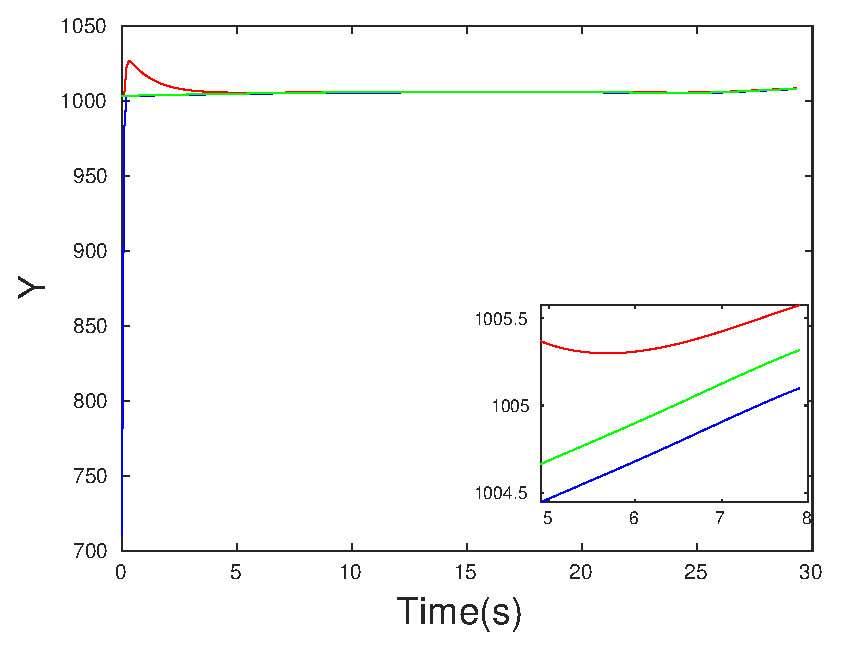
\includegraphics[width=\linewidth]{figures/Prad/s3cvpradY}
\end{subfigure}
\begin{subfigure}{.5\linewidth}
\centering
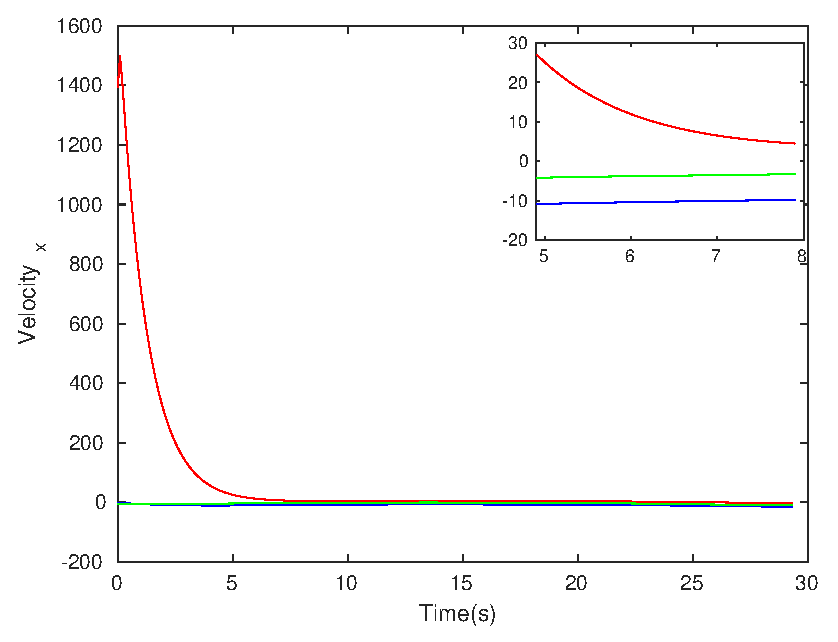
\includegraphics[width=.9\linewidth]{figures/Prad/s3cvpradVelocity_x}
\end{subfigure}
\begin{subfigure}{.5\linewidth}
\centering
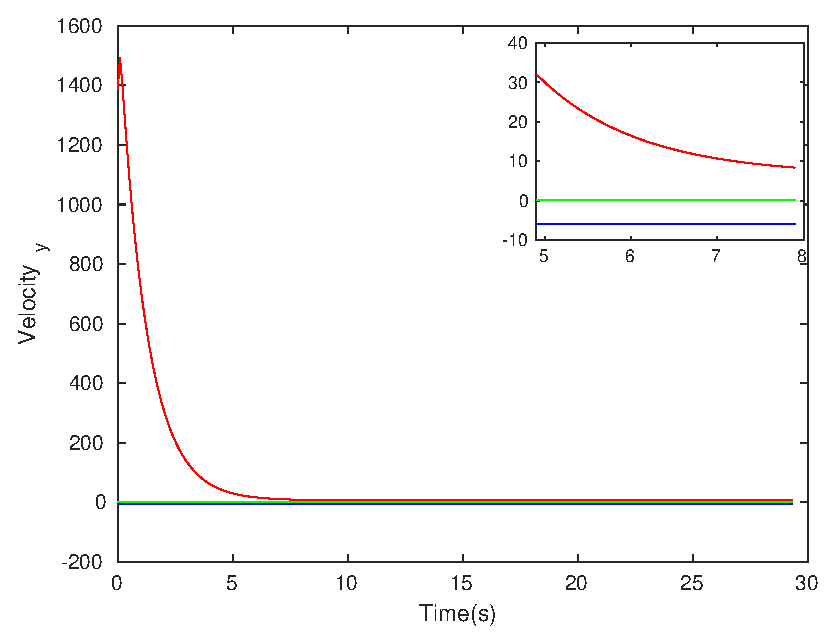
\includegraphics[width=.9\linewidth]{figures/Prad/s3cvpradVelocity_y}
\end{subfigure}
\caption{Estimation using Constant Velocity}
\end{figure}

\begin{figure}[h]
\begin{subfigure}{.5\linewidth}
\centering
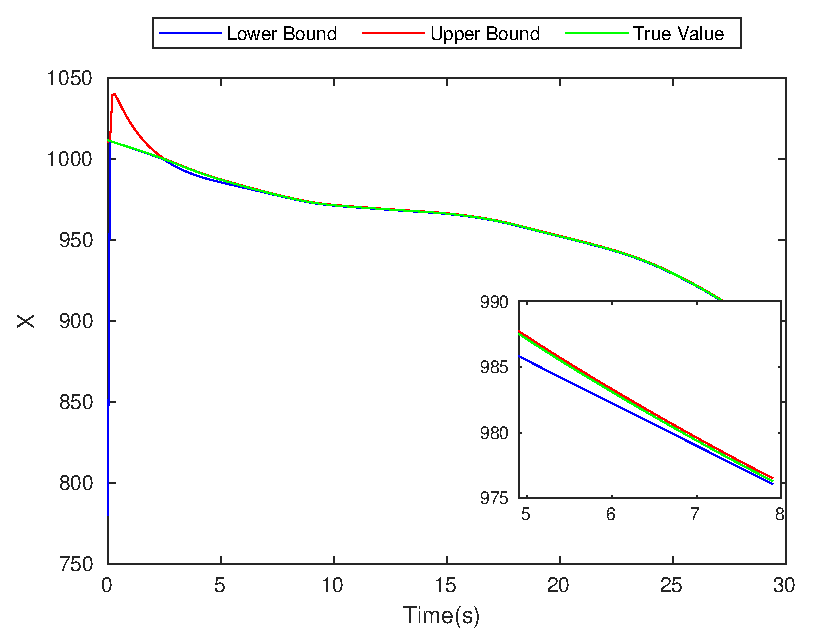
\includegraphics[width=\linewidth]{figures/Prad/s3capradX}
\end{subfigure}
\begin{subfigure}{.5\linewidth}
\centering
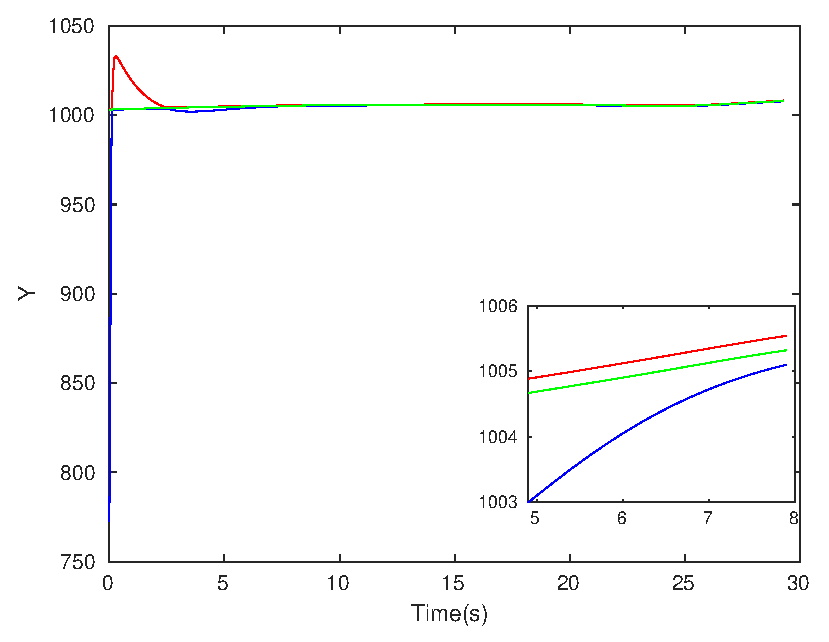
\includegraphics[width=\linewidth]{figures/Prad/s3capradY}
\end{subfigure}
\begin{subfigure}{.5\linewidth}
\centering
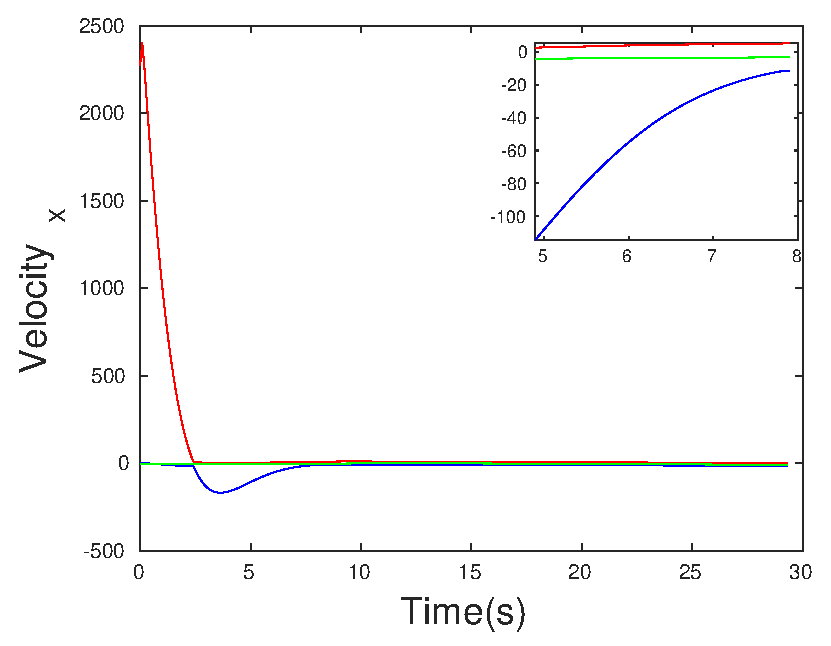
\includegraphics[width=.9\linewidth]{figures/Prad/s3capradVelocity_x}
\end{subfigure}
\begin{subfigure}{.5\linewidth}
\centering
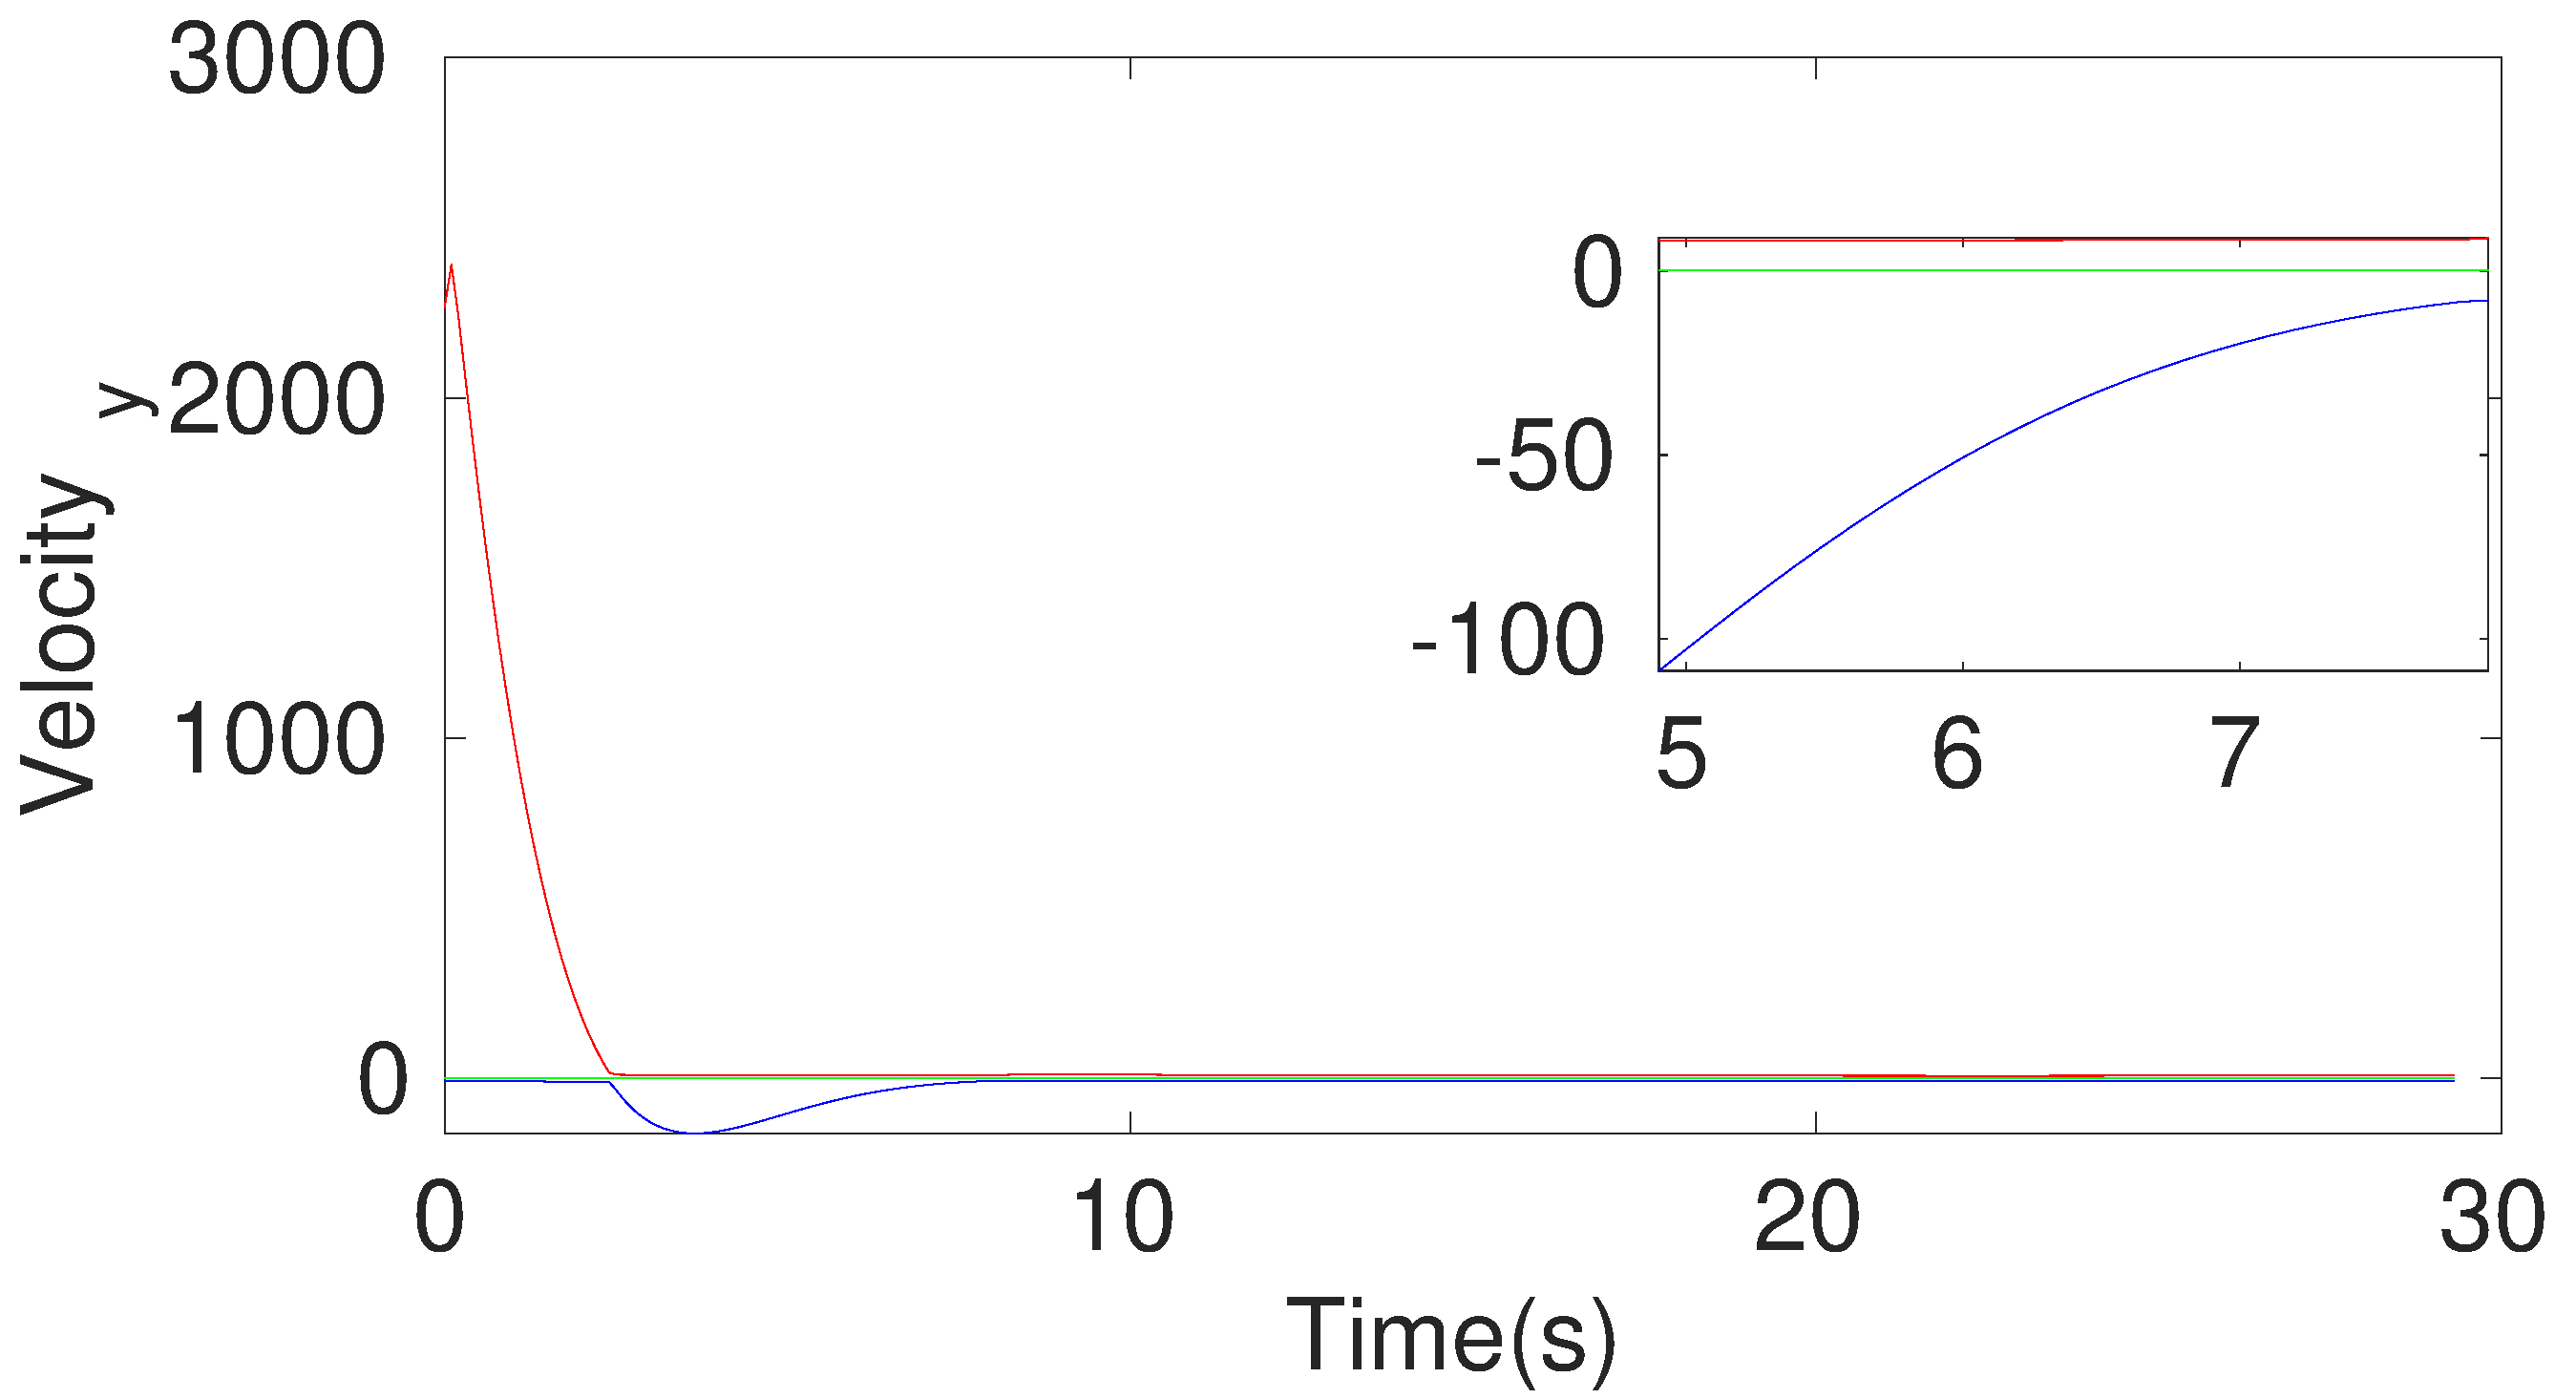
\includegraphics[width=.9\linewidth]{figures/Prad/s3capradVelocity_y}
\end{subfigure}
\begin{subfigure}{.5\linewidth}
\centering
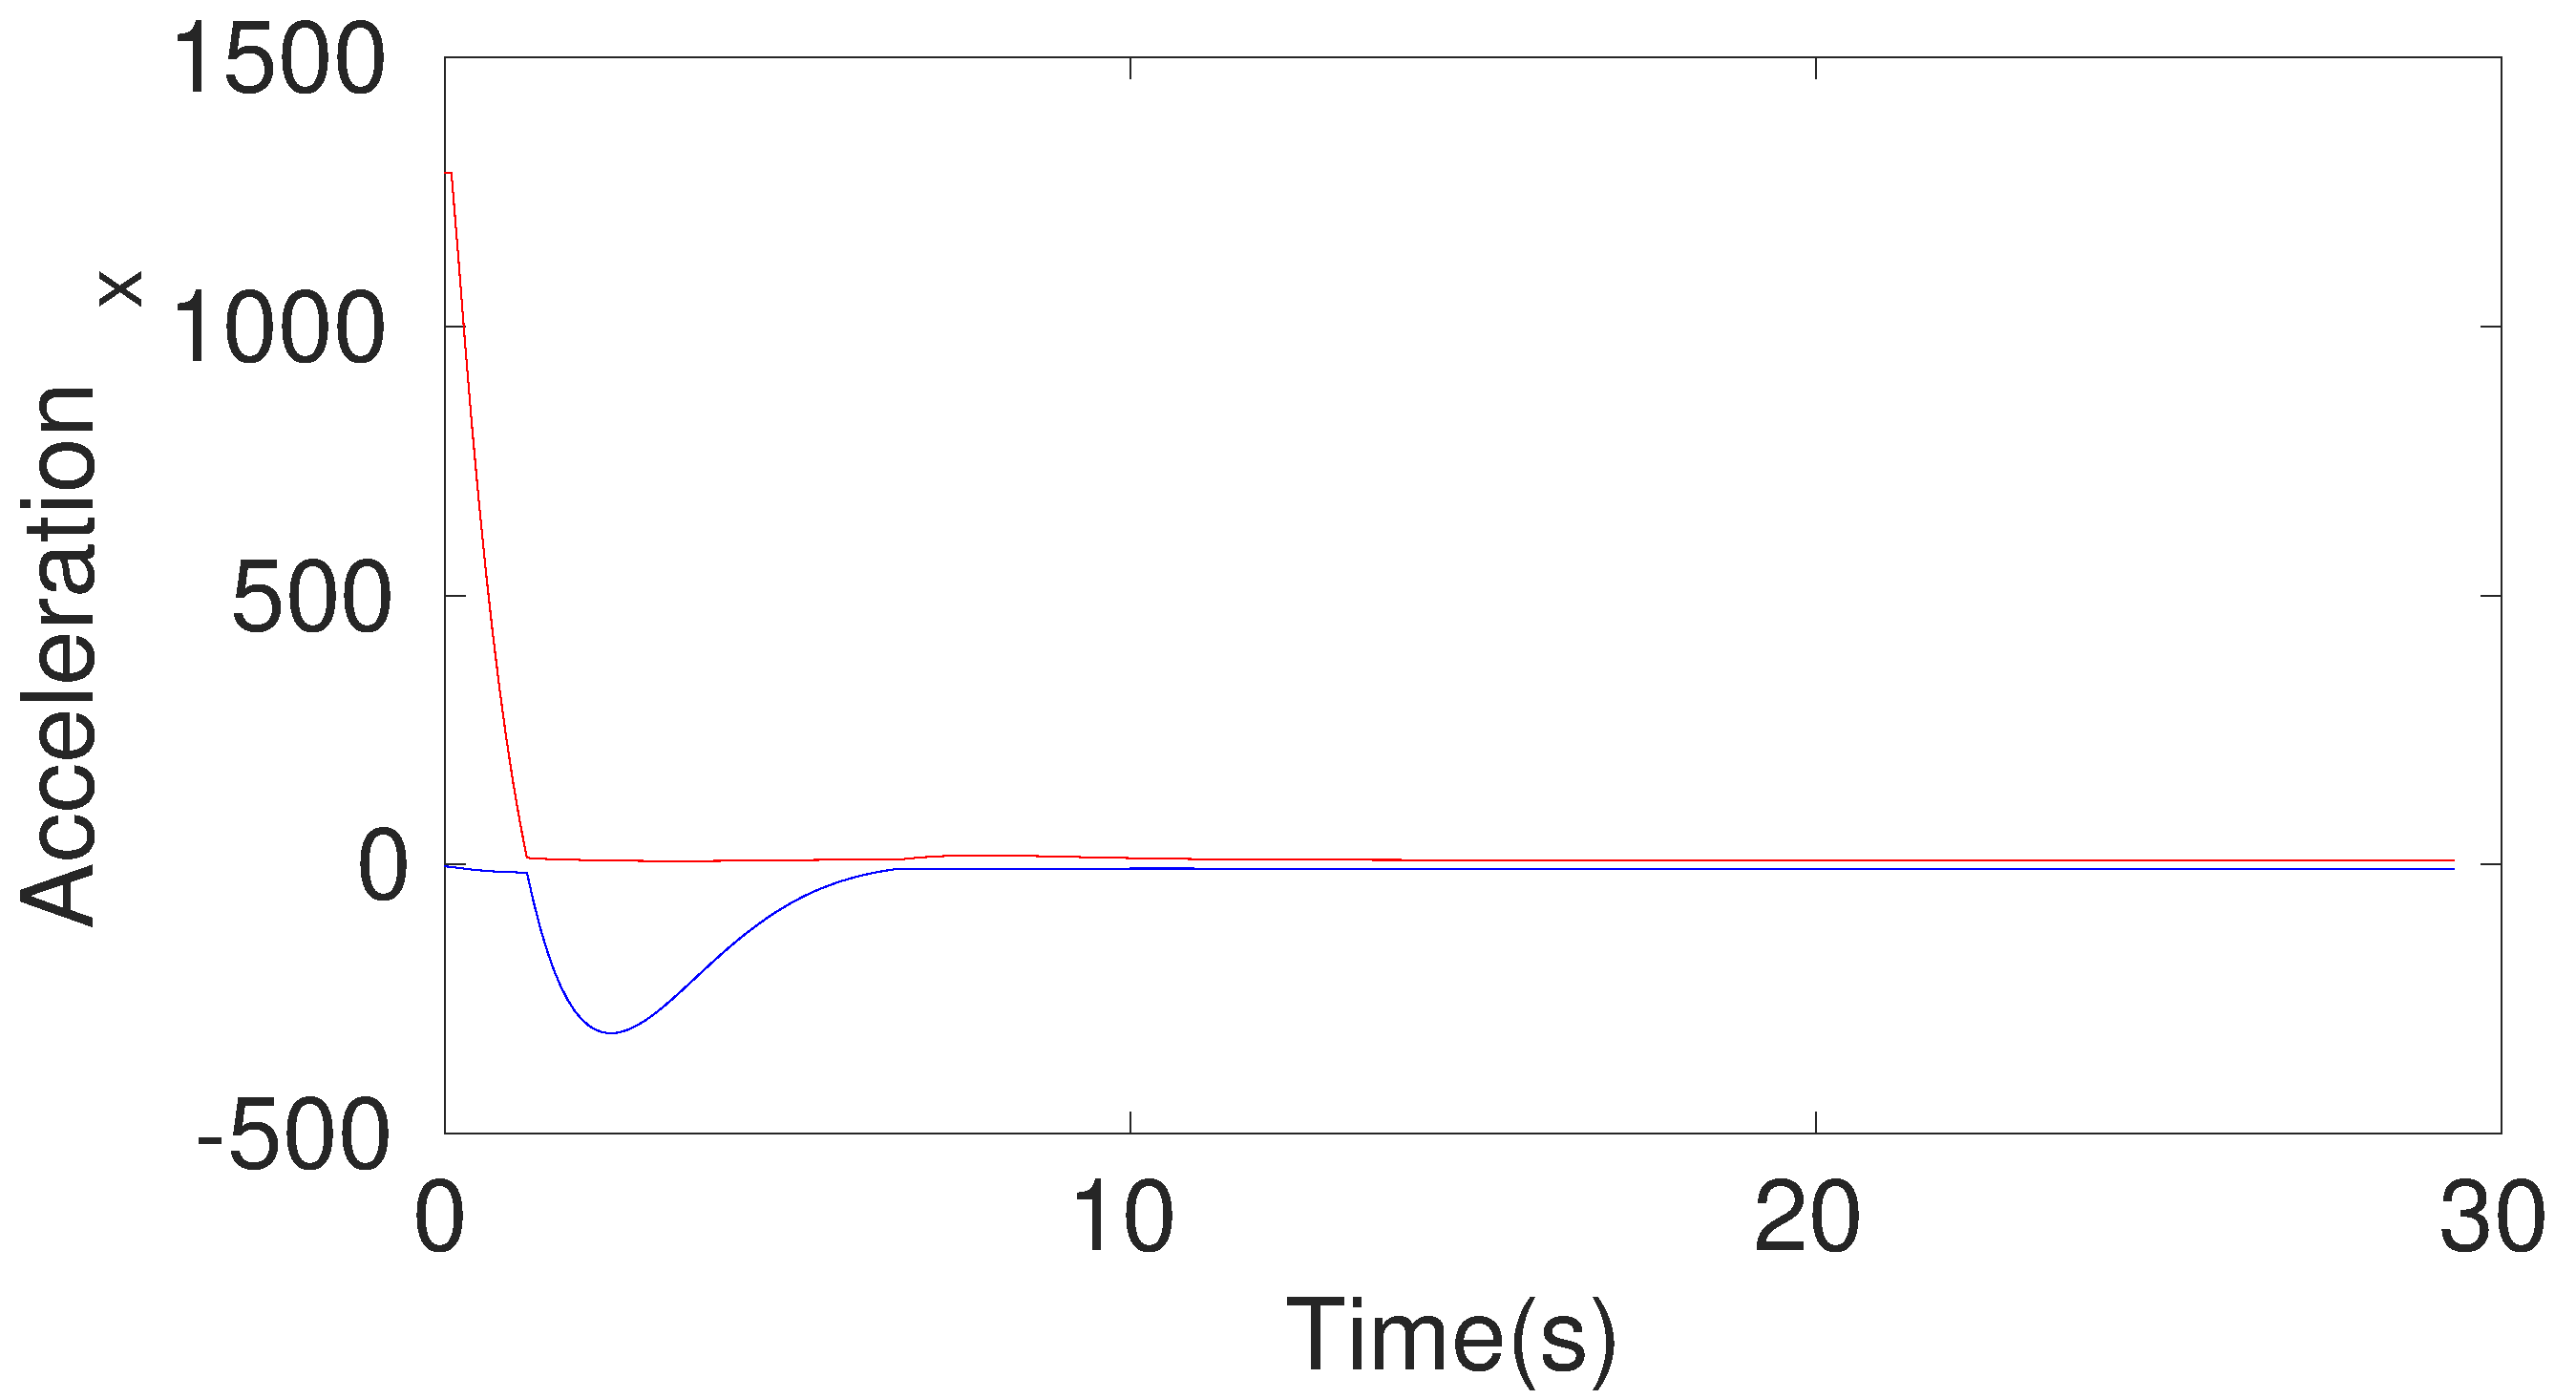
\includegraphics[width=.9\linewidth]{figures/Prad/s3capradAcceleration_x}
\end{subfigure}
\begin{subfigure}{.5\linewidth}
\centering
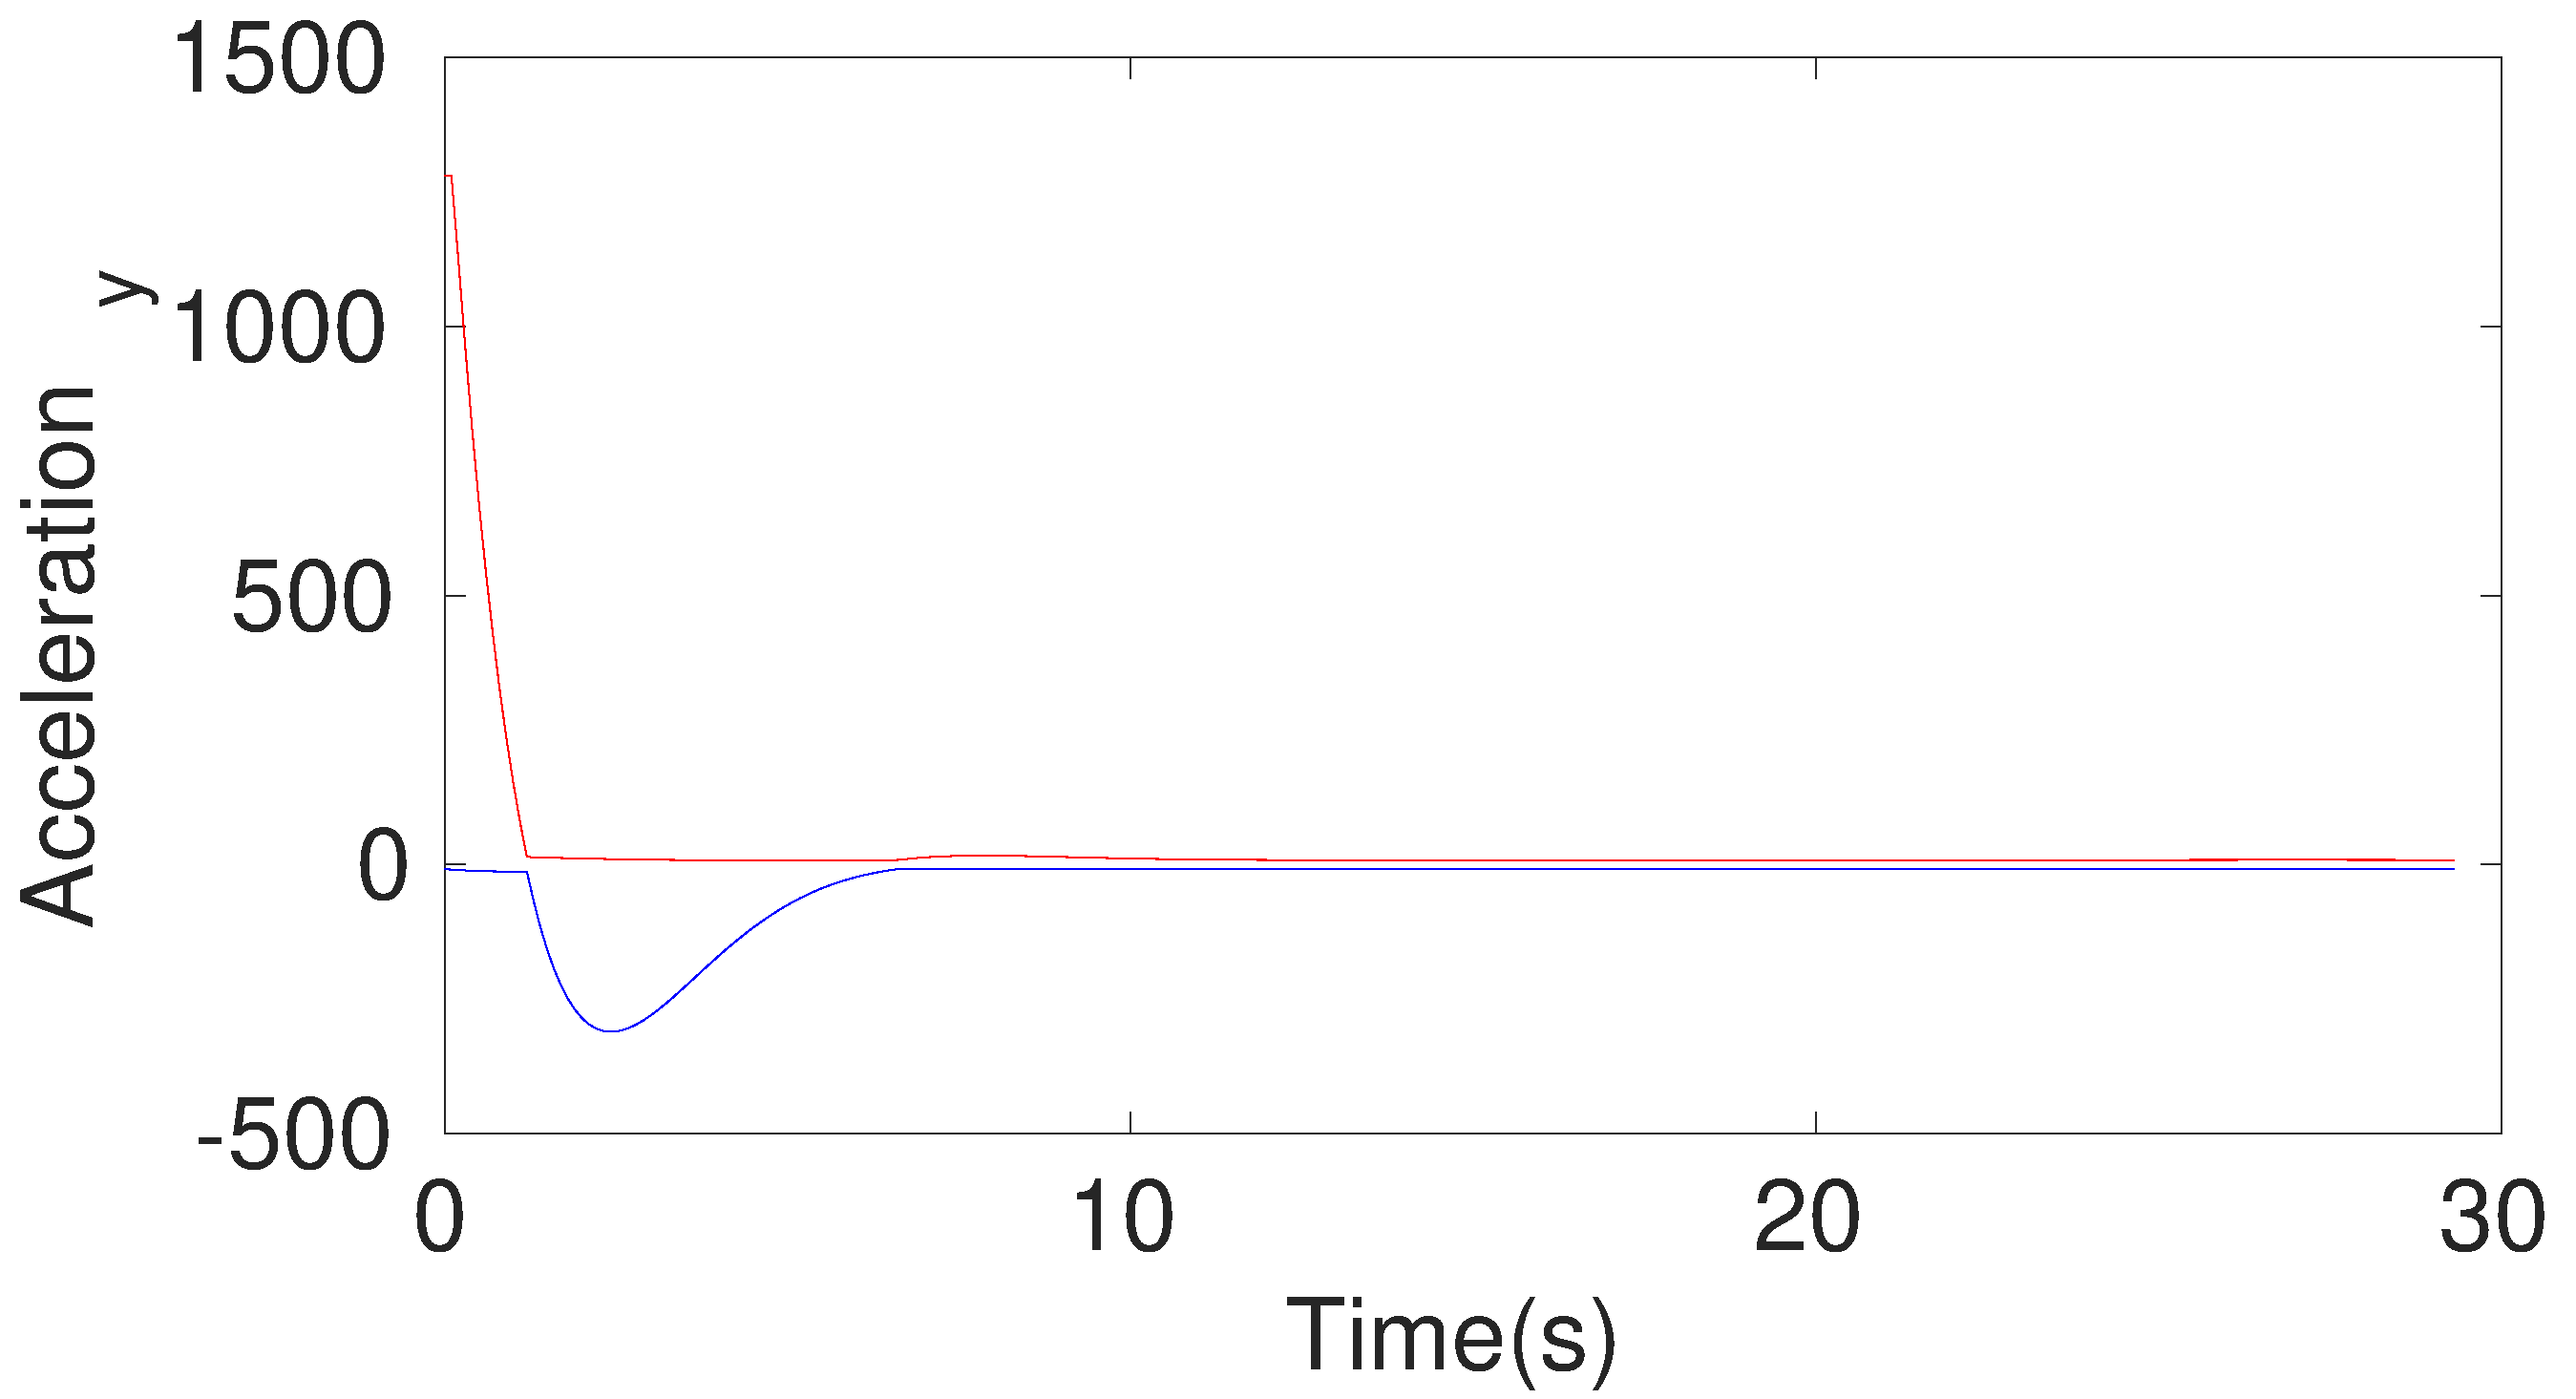
\includegraphics[width=.9\linewidth]{figures/Prad/s3capradAcceleration_y}
\end{subfigure}
\caption{Estimation using Constant Acceleration}
\end{figure}
\begin{figure}[h]
\begin{subfigure}{.5\linewidth}
\centering
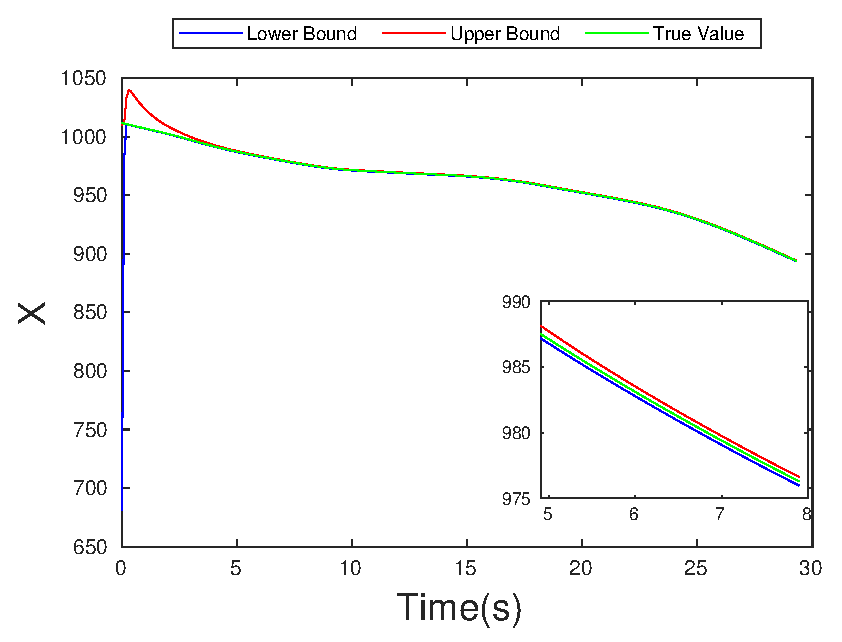
\includegraphics[width=\linewidth]{figures/Prad/s3cspradX}
\end{subfigure}
\begin{subfigure}{.5\linewidth}
\centering
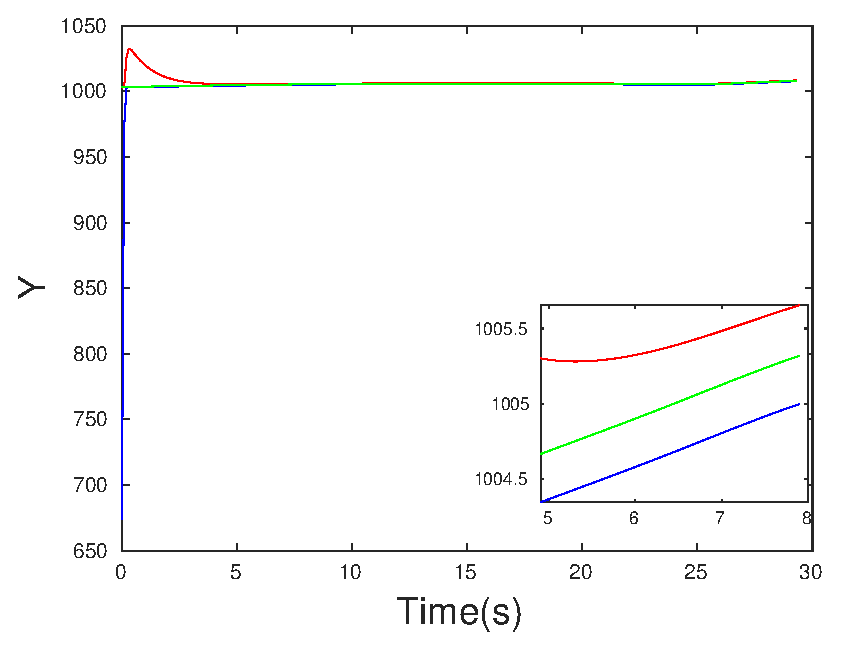
\includegraphics[width=\linewidth]{figures/Prad/s3cspradY}
\end{subfigure}
\begin{subfigure}{.5\linewidth}
\centering
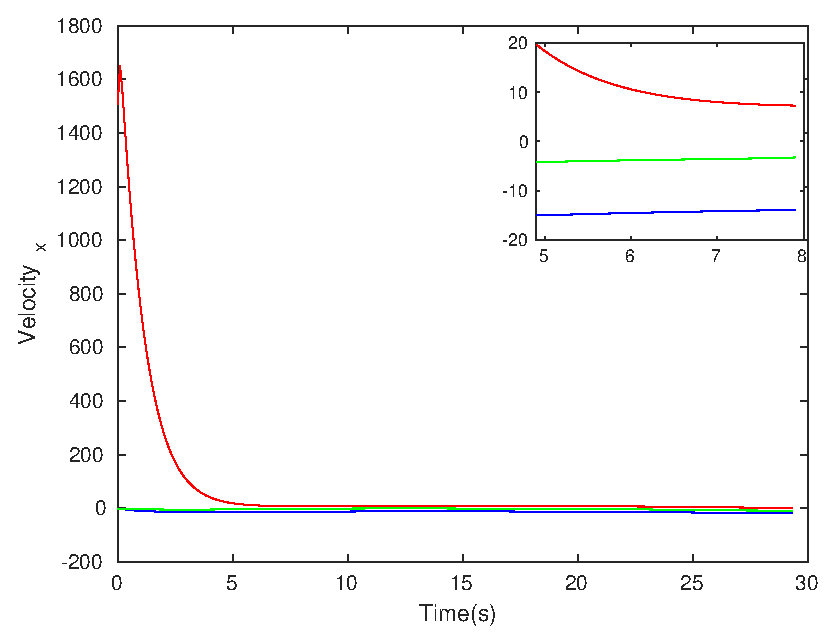
\includegraphics[width=.9\linewidth]{figures/Prad/s3cspradVelocity_x}
\end{subfigure}
\begin{subfigure}{.5\linewidth}
\centering
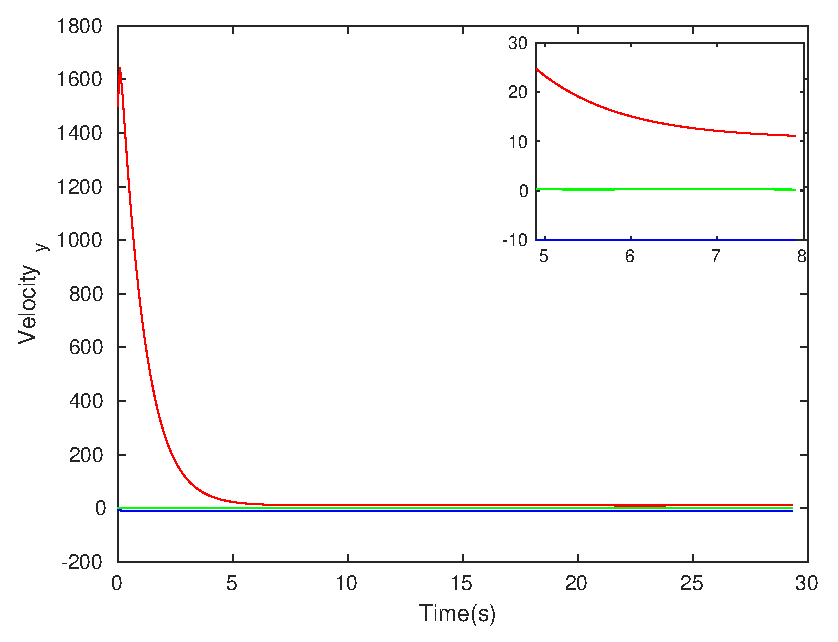
\includegraphics[width=.9\linewidth]{figures/Prad/s3cspradVelocity_y}
\end{subfigure}
\begin{subfigure}{.5\linewidth}
\centering
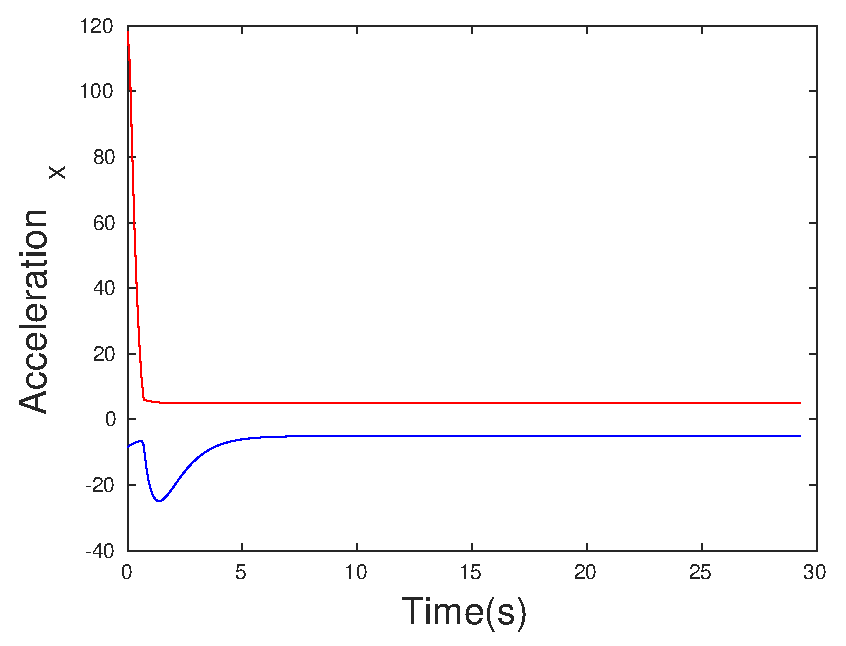
\includegraphics[width=.9\linewidth]{figures/Prad/s3cspradAcceleration_x}
\end{subfigure}
\begin{subfigure}{.5\linewidth}
\centering
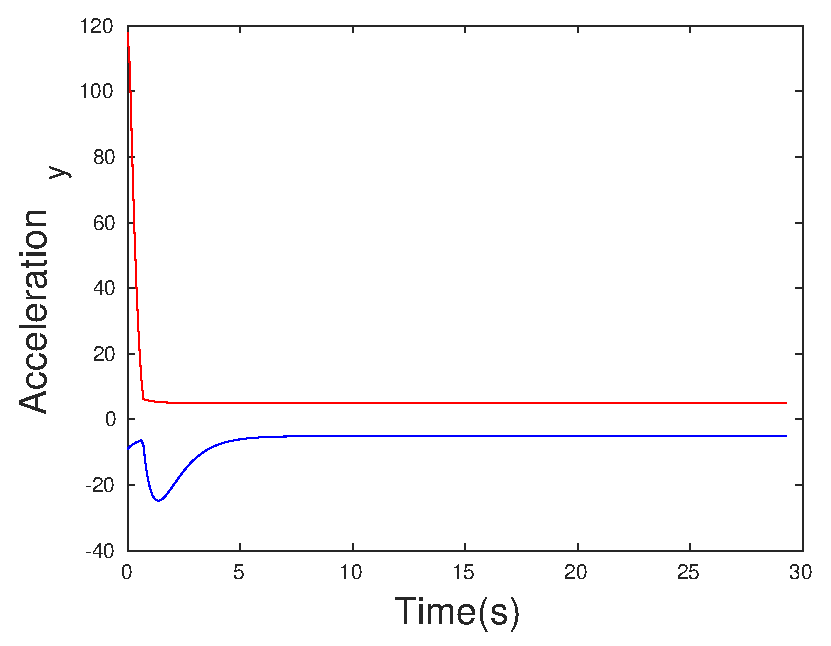
\includegraphics[width=.9\linewidth]{figures/Prad/s3cspradAcceleration_y}
\end{subfigure}
\caption{Estimation using Singer Acceleration}
\end{figure}



\subsection{Segment Minimization using H-$\infty$}
\FloatBarrier
\begin{figure}[h]
\begin{subfigure}{.5\linewidth}
\centering
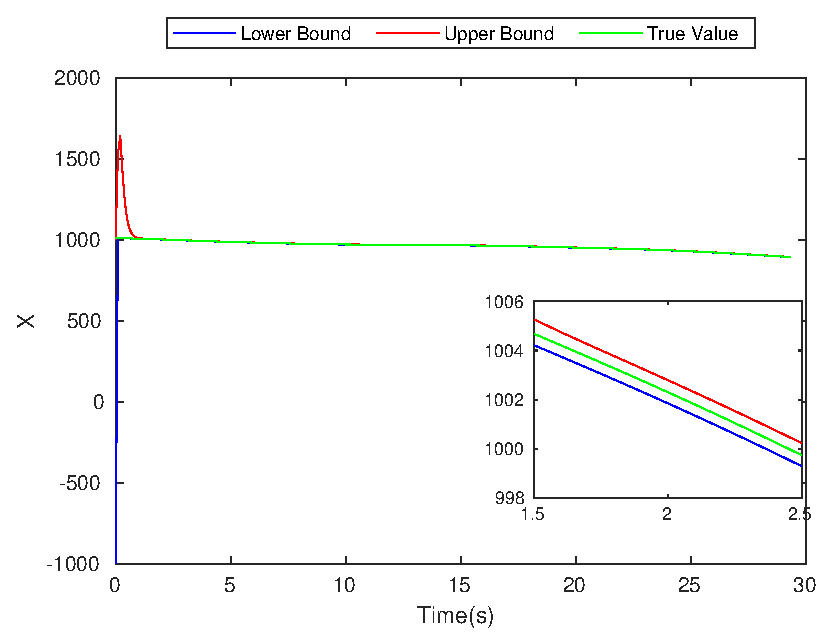
\includegraphics[width=\linewidth]{figures/HInf/s3cvHInfX}
\end{subfigure}
\begin{subfigure}{.5\linewidth}
\centering
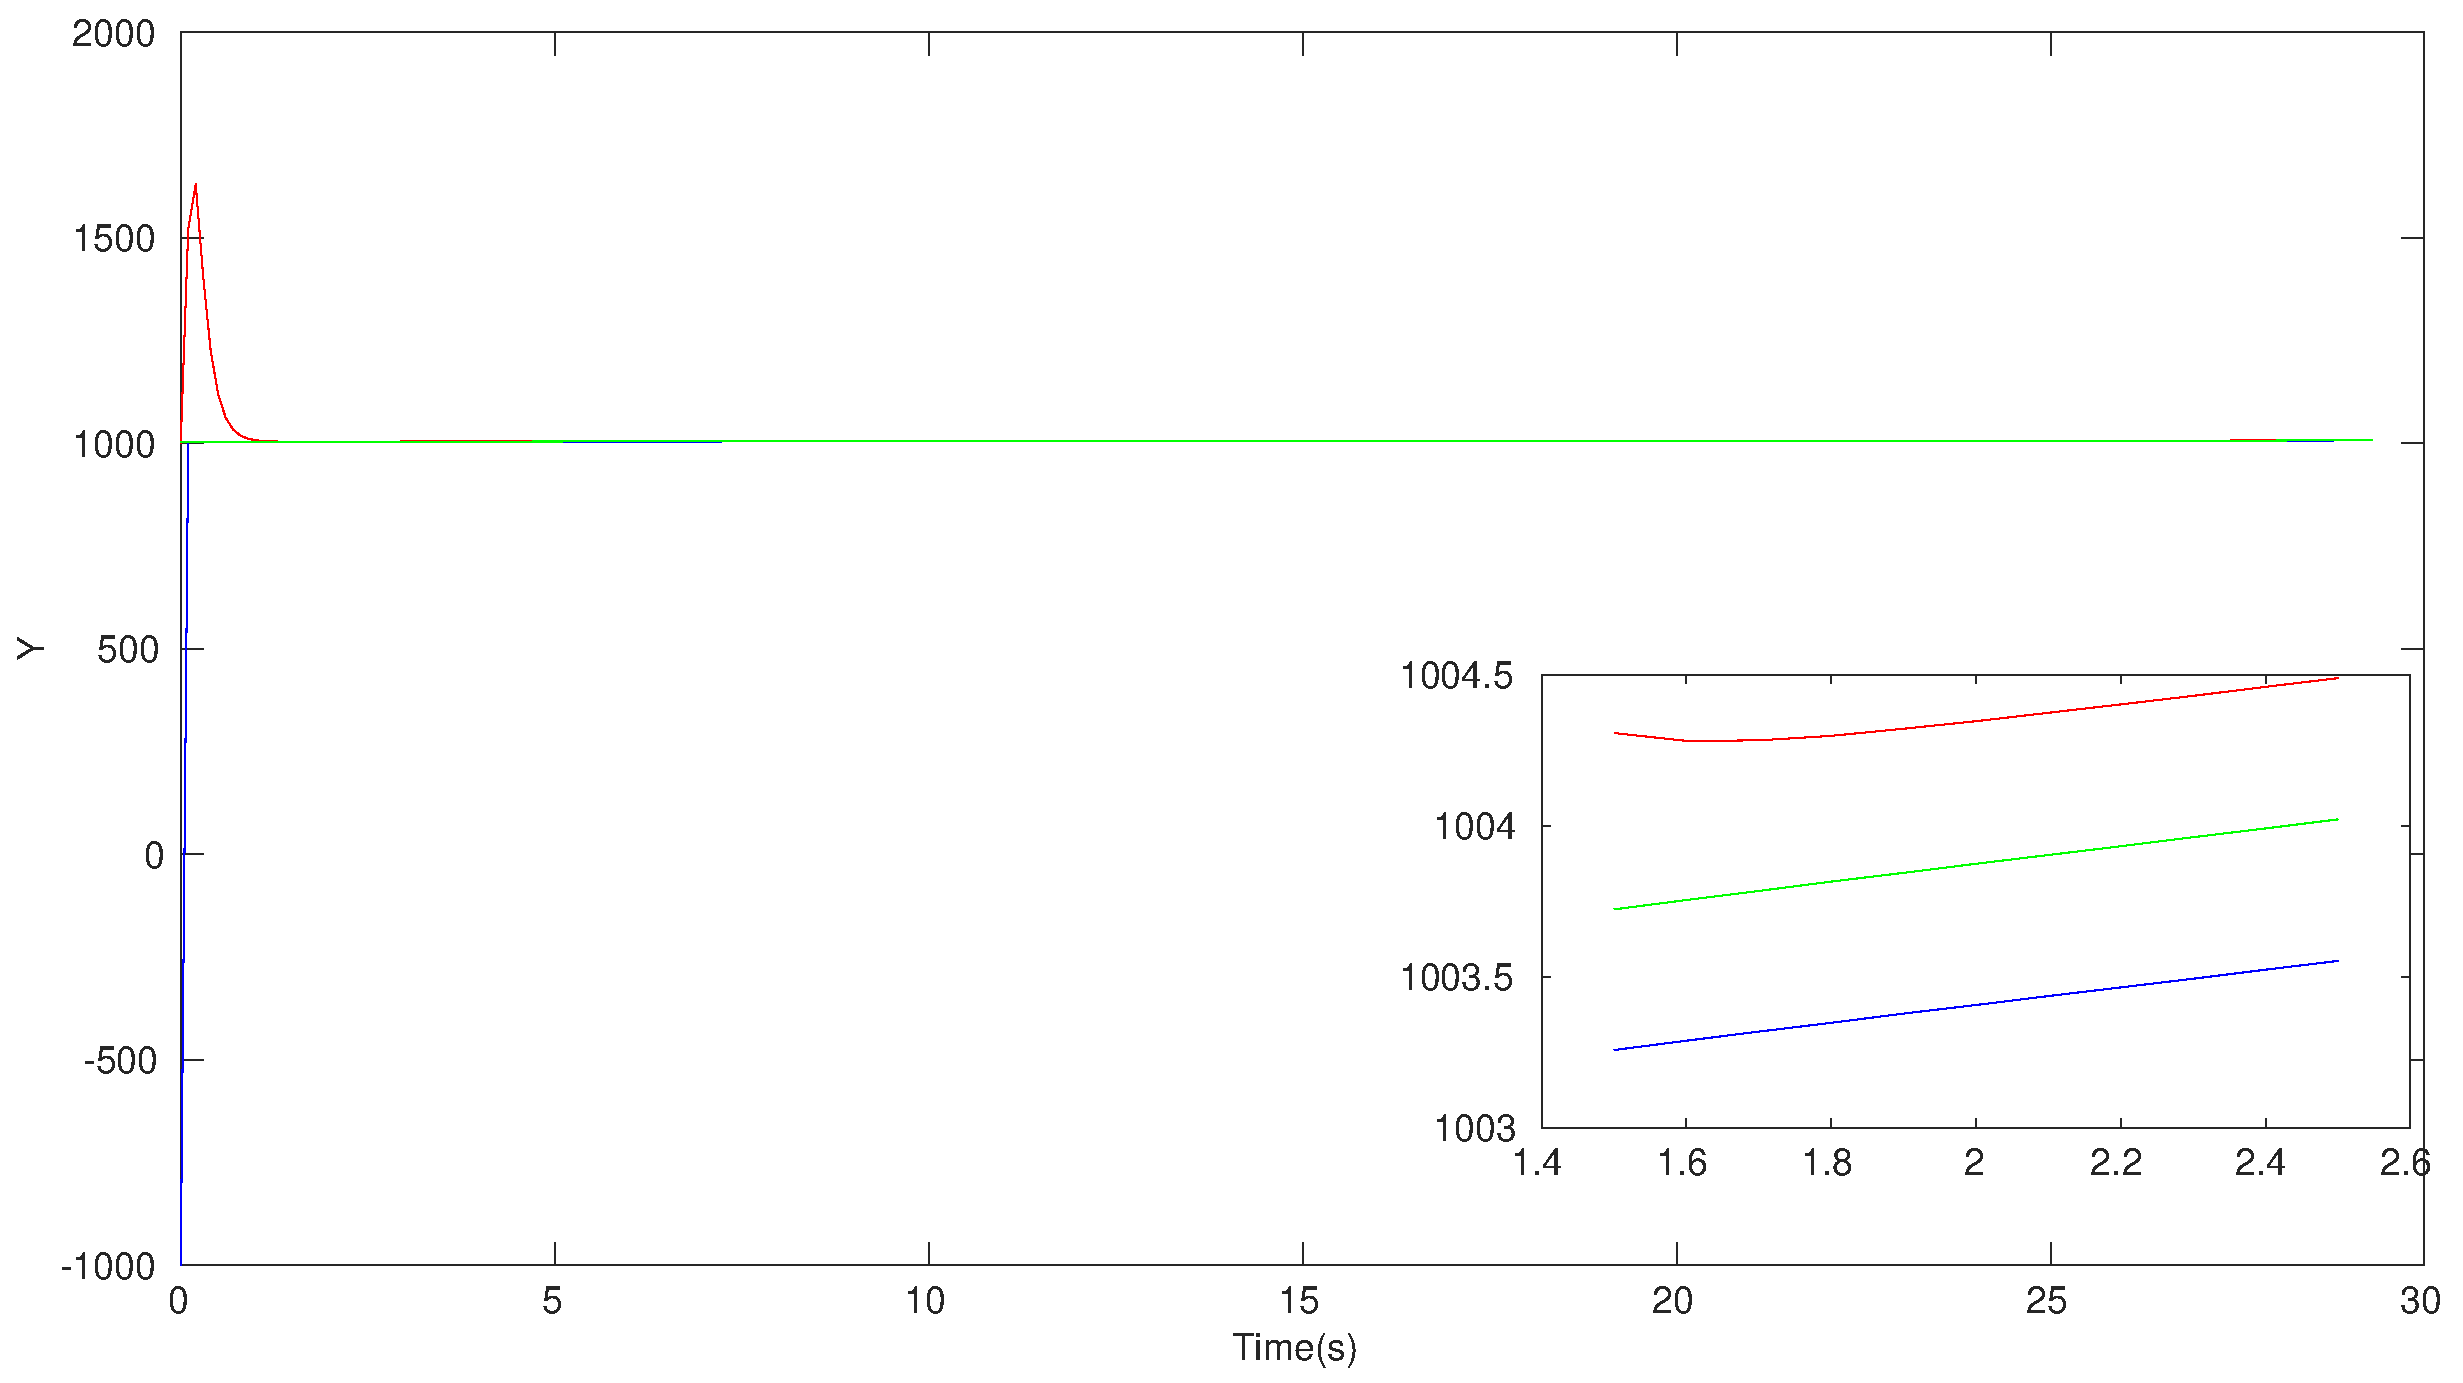
\includegraphics[width=\linewidth]{figures/HInf/s3cvHInfY}
\end{subfigure}
\begin{subfigure}{.5\linewidth}
\centering
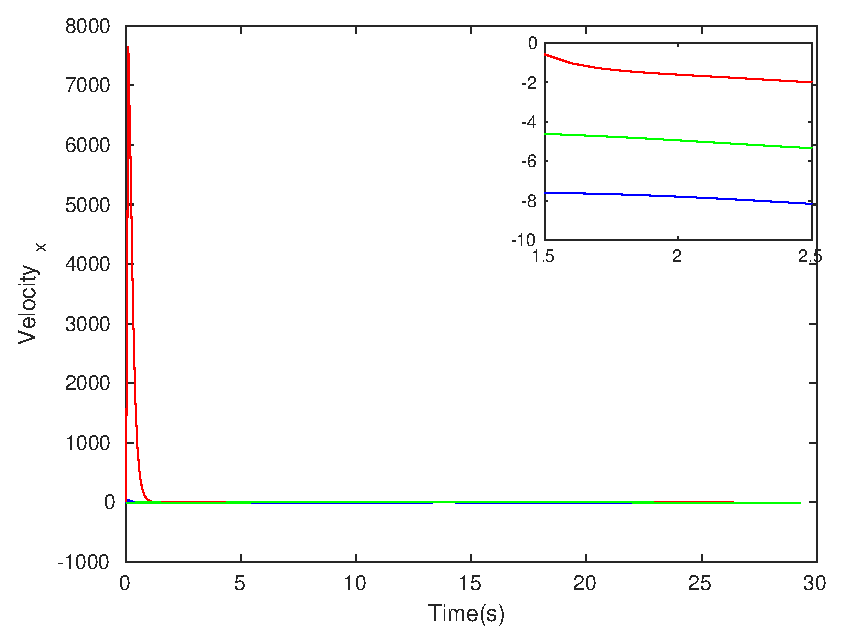
\includegraphics[width=.9\linewidth]{figures/HInf/s3cvHInfVelocity_x}
\end{subfigure}
\begin{subfigure}{.5\linewidth}
\centering
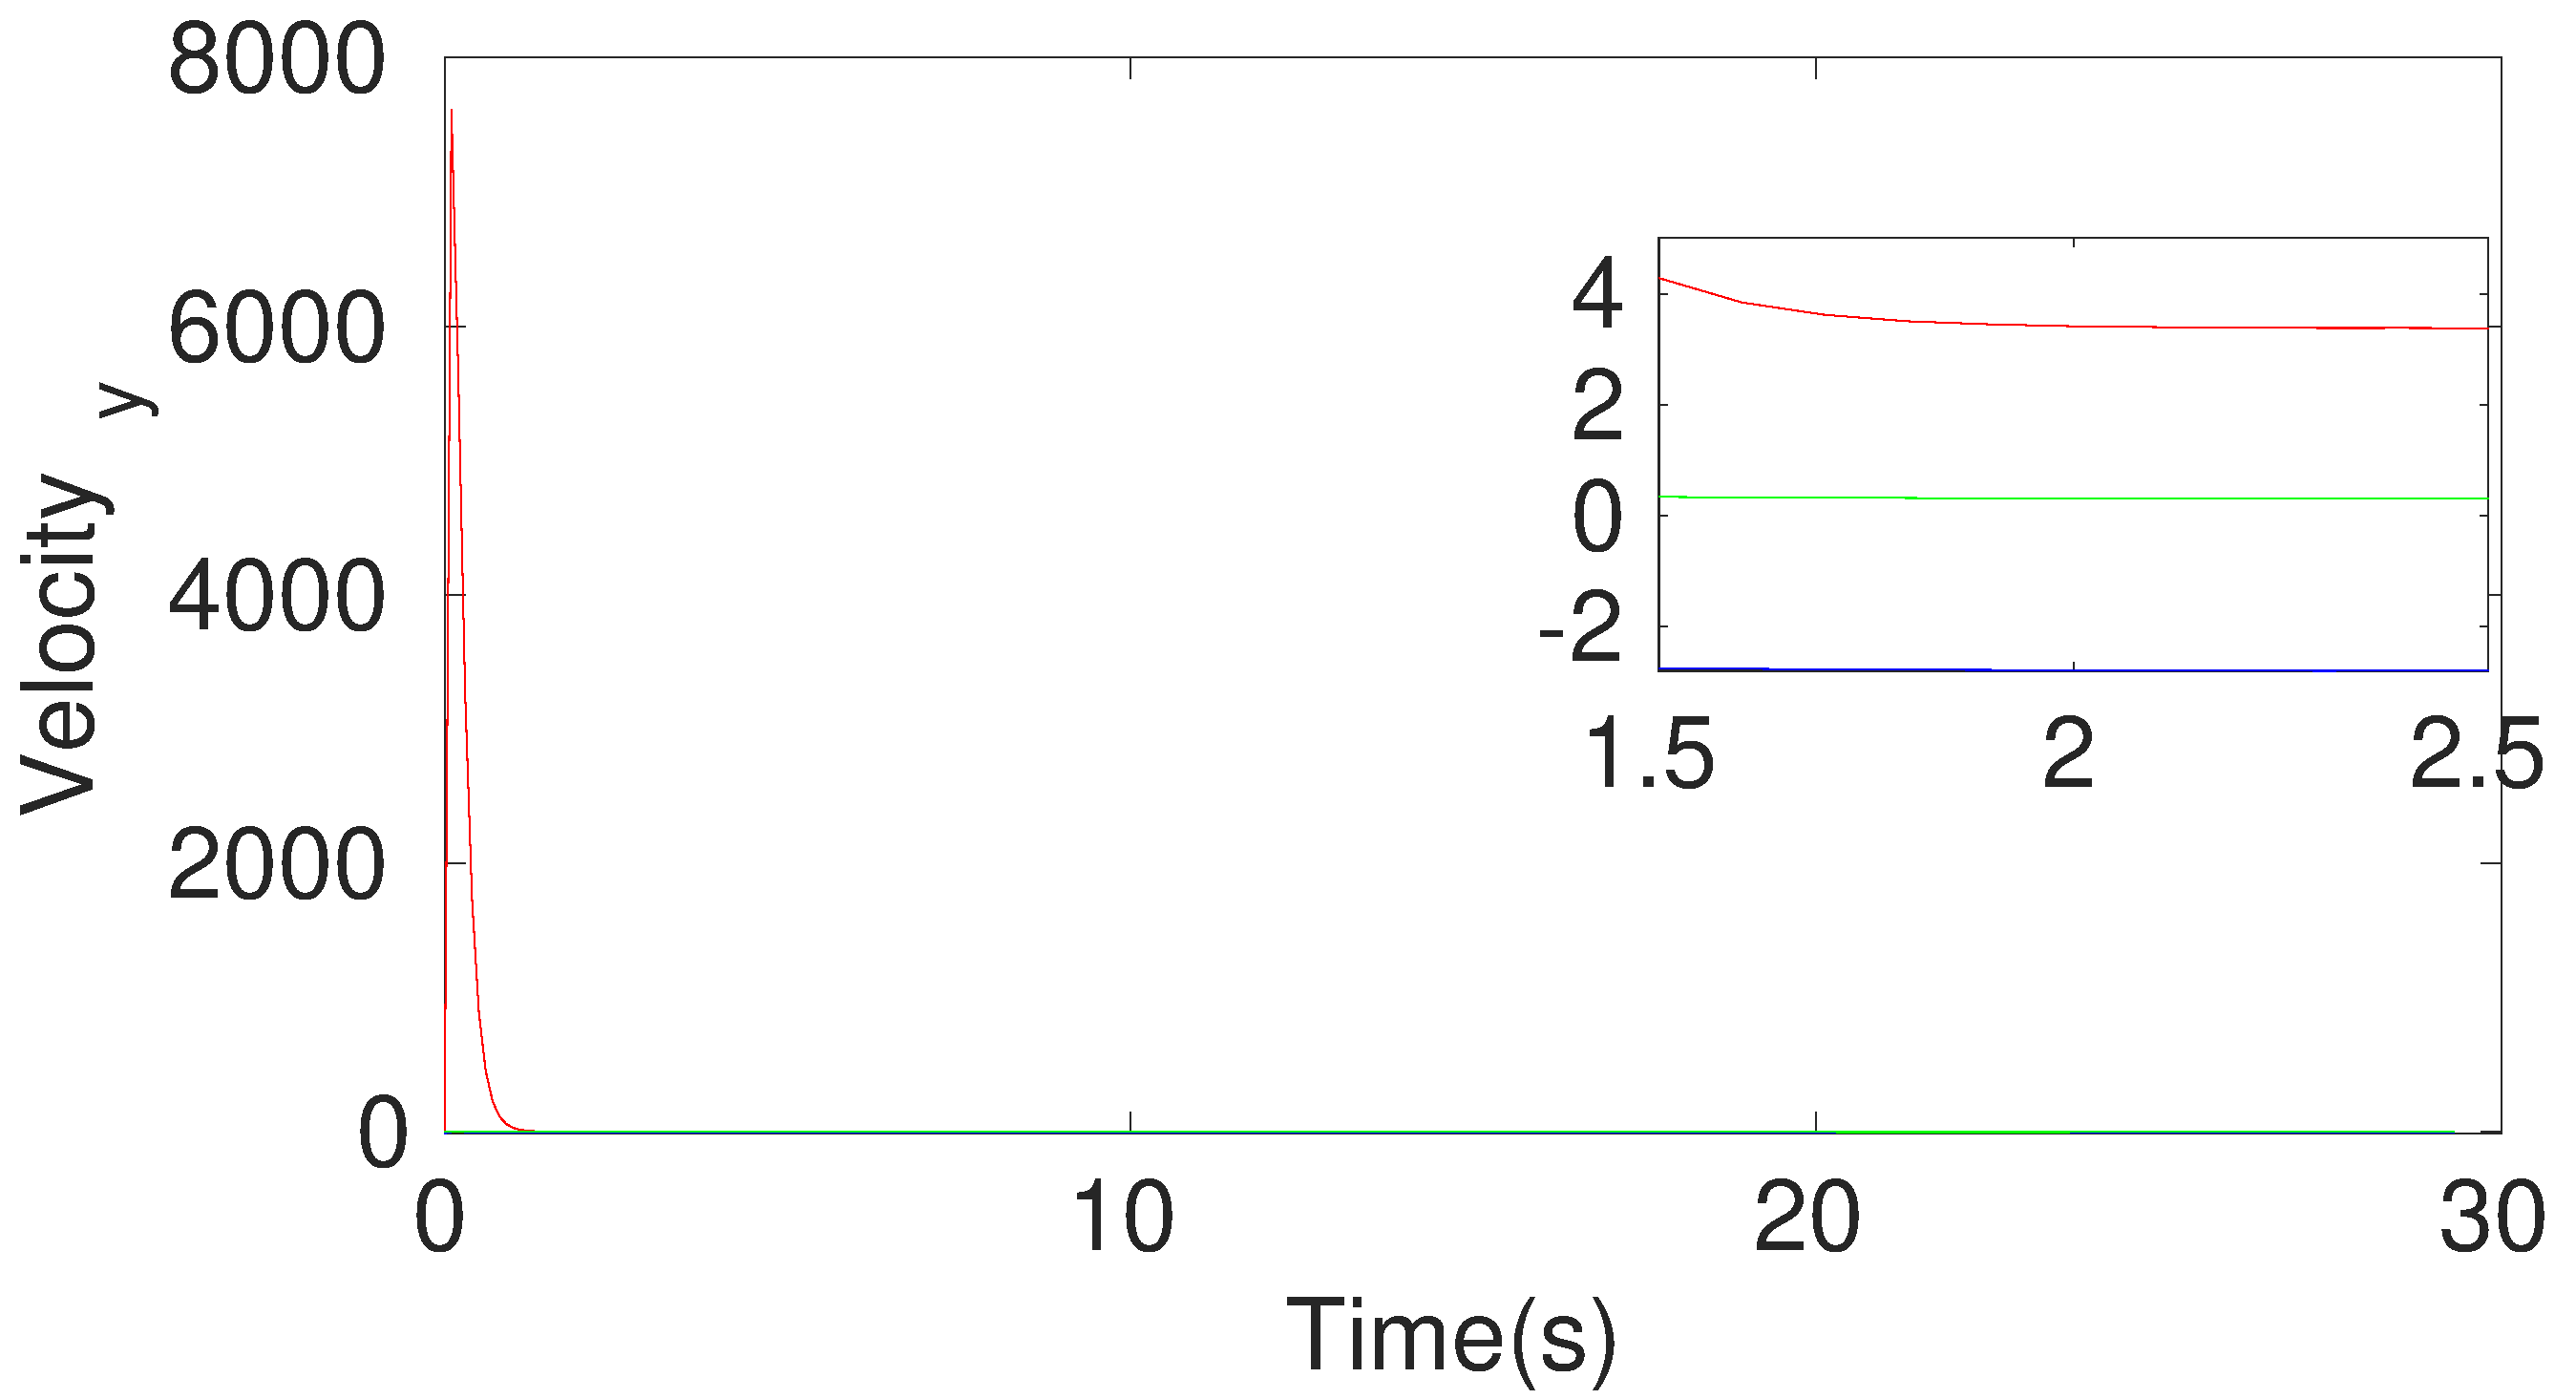
\includegraphics[width=.9\linewidth]{figures/HInf/s3cvHInfVelocity_y}
\end{subfigure}
\caption{Estimation using Constant Velocity}
\end{figure}

\begin{figure}[h]
\begin{subfigure}{.5\linewidth}
\centering
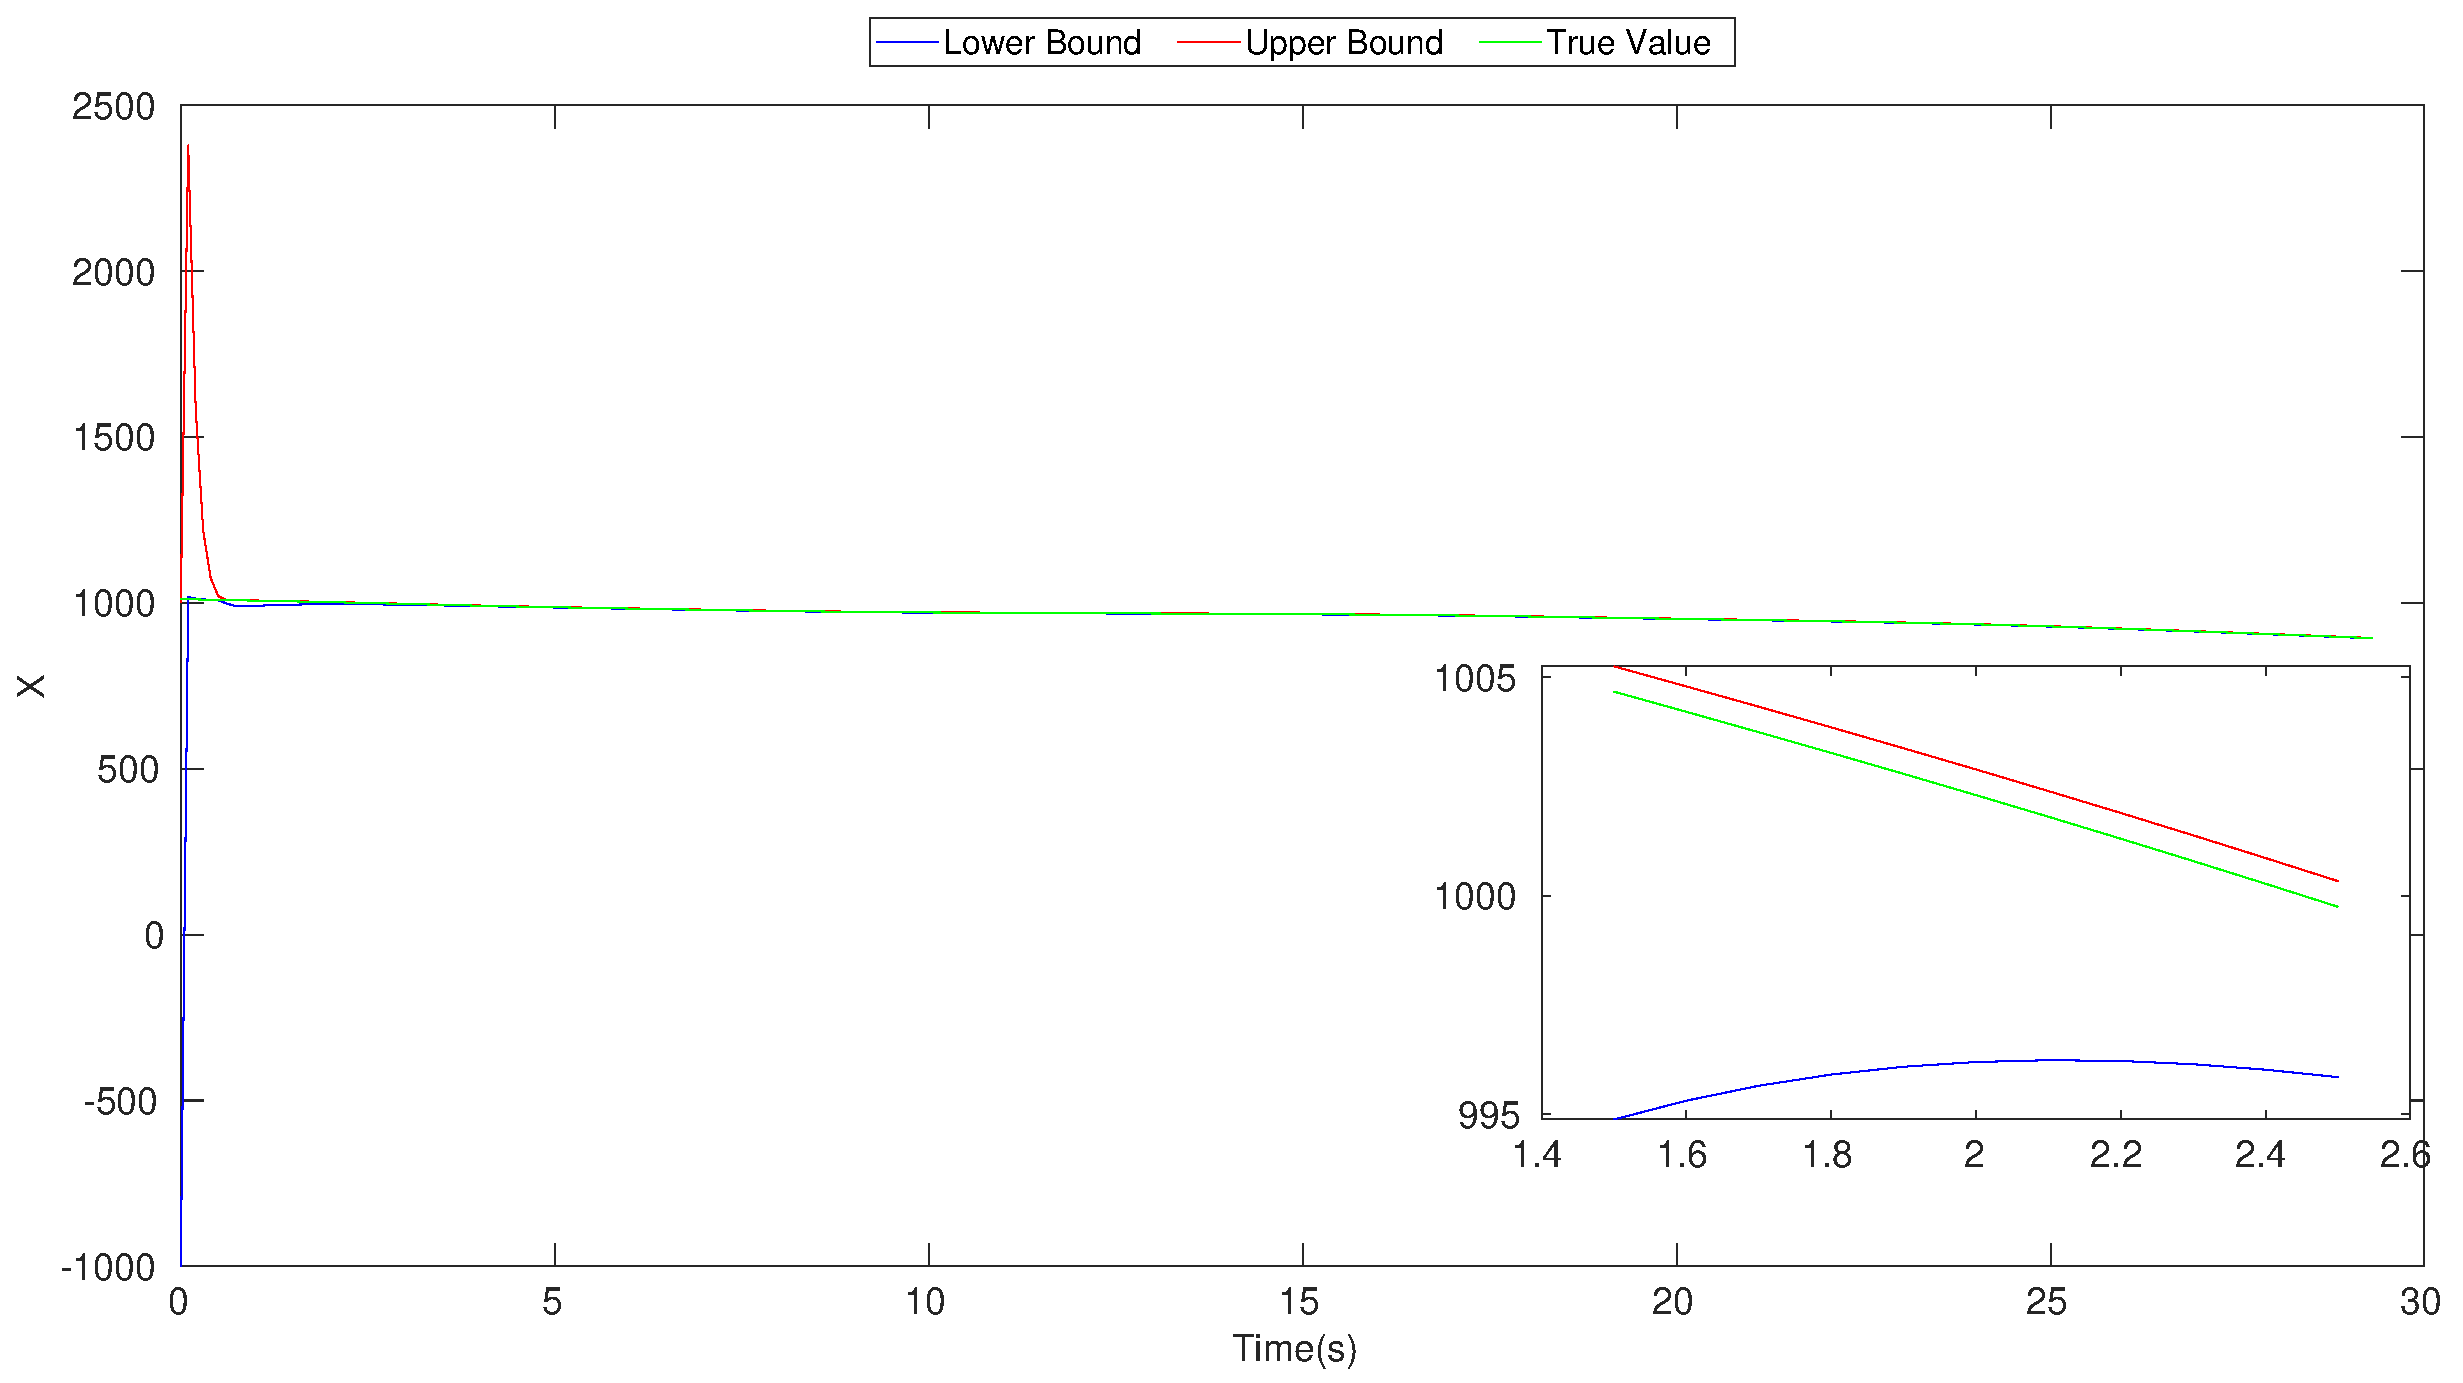
\includegraphics[width=\linewidth]{figures/HInf/s3caHInfX}
\end{subfigure}
\begin{subfigure}{.5\linewidth}
\centering
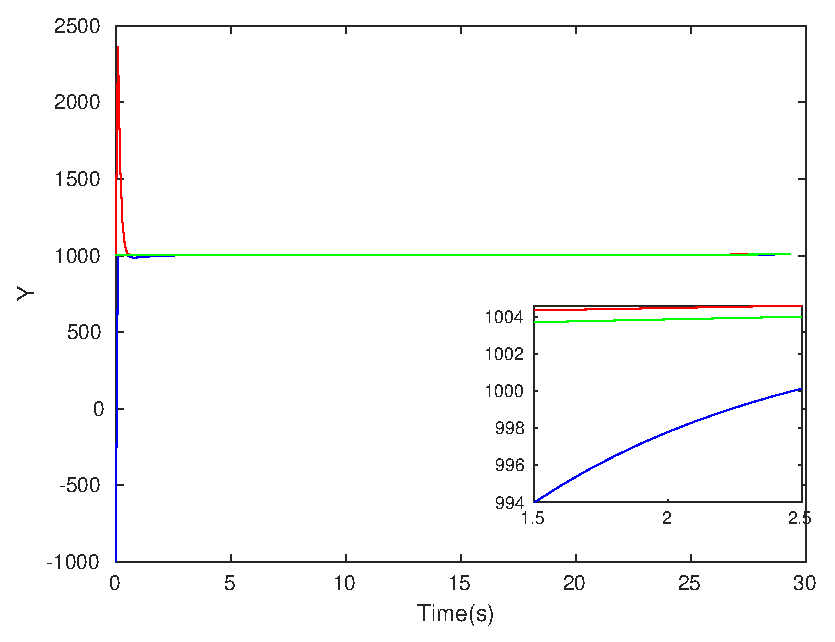
\includegraphics[width=\linewidth]{figures/HInf/s3caHInfY}
\end{subfigure}
\begin{subfigure}{.5\linewidth}
\centering
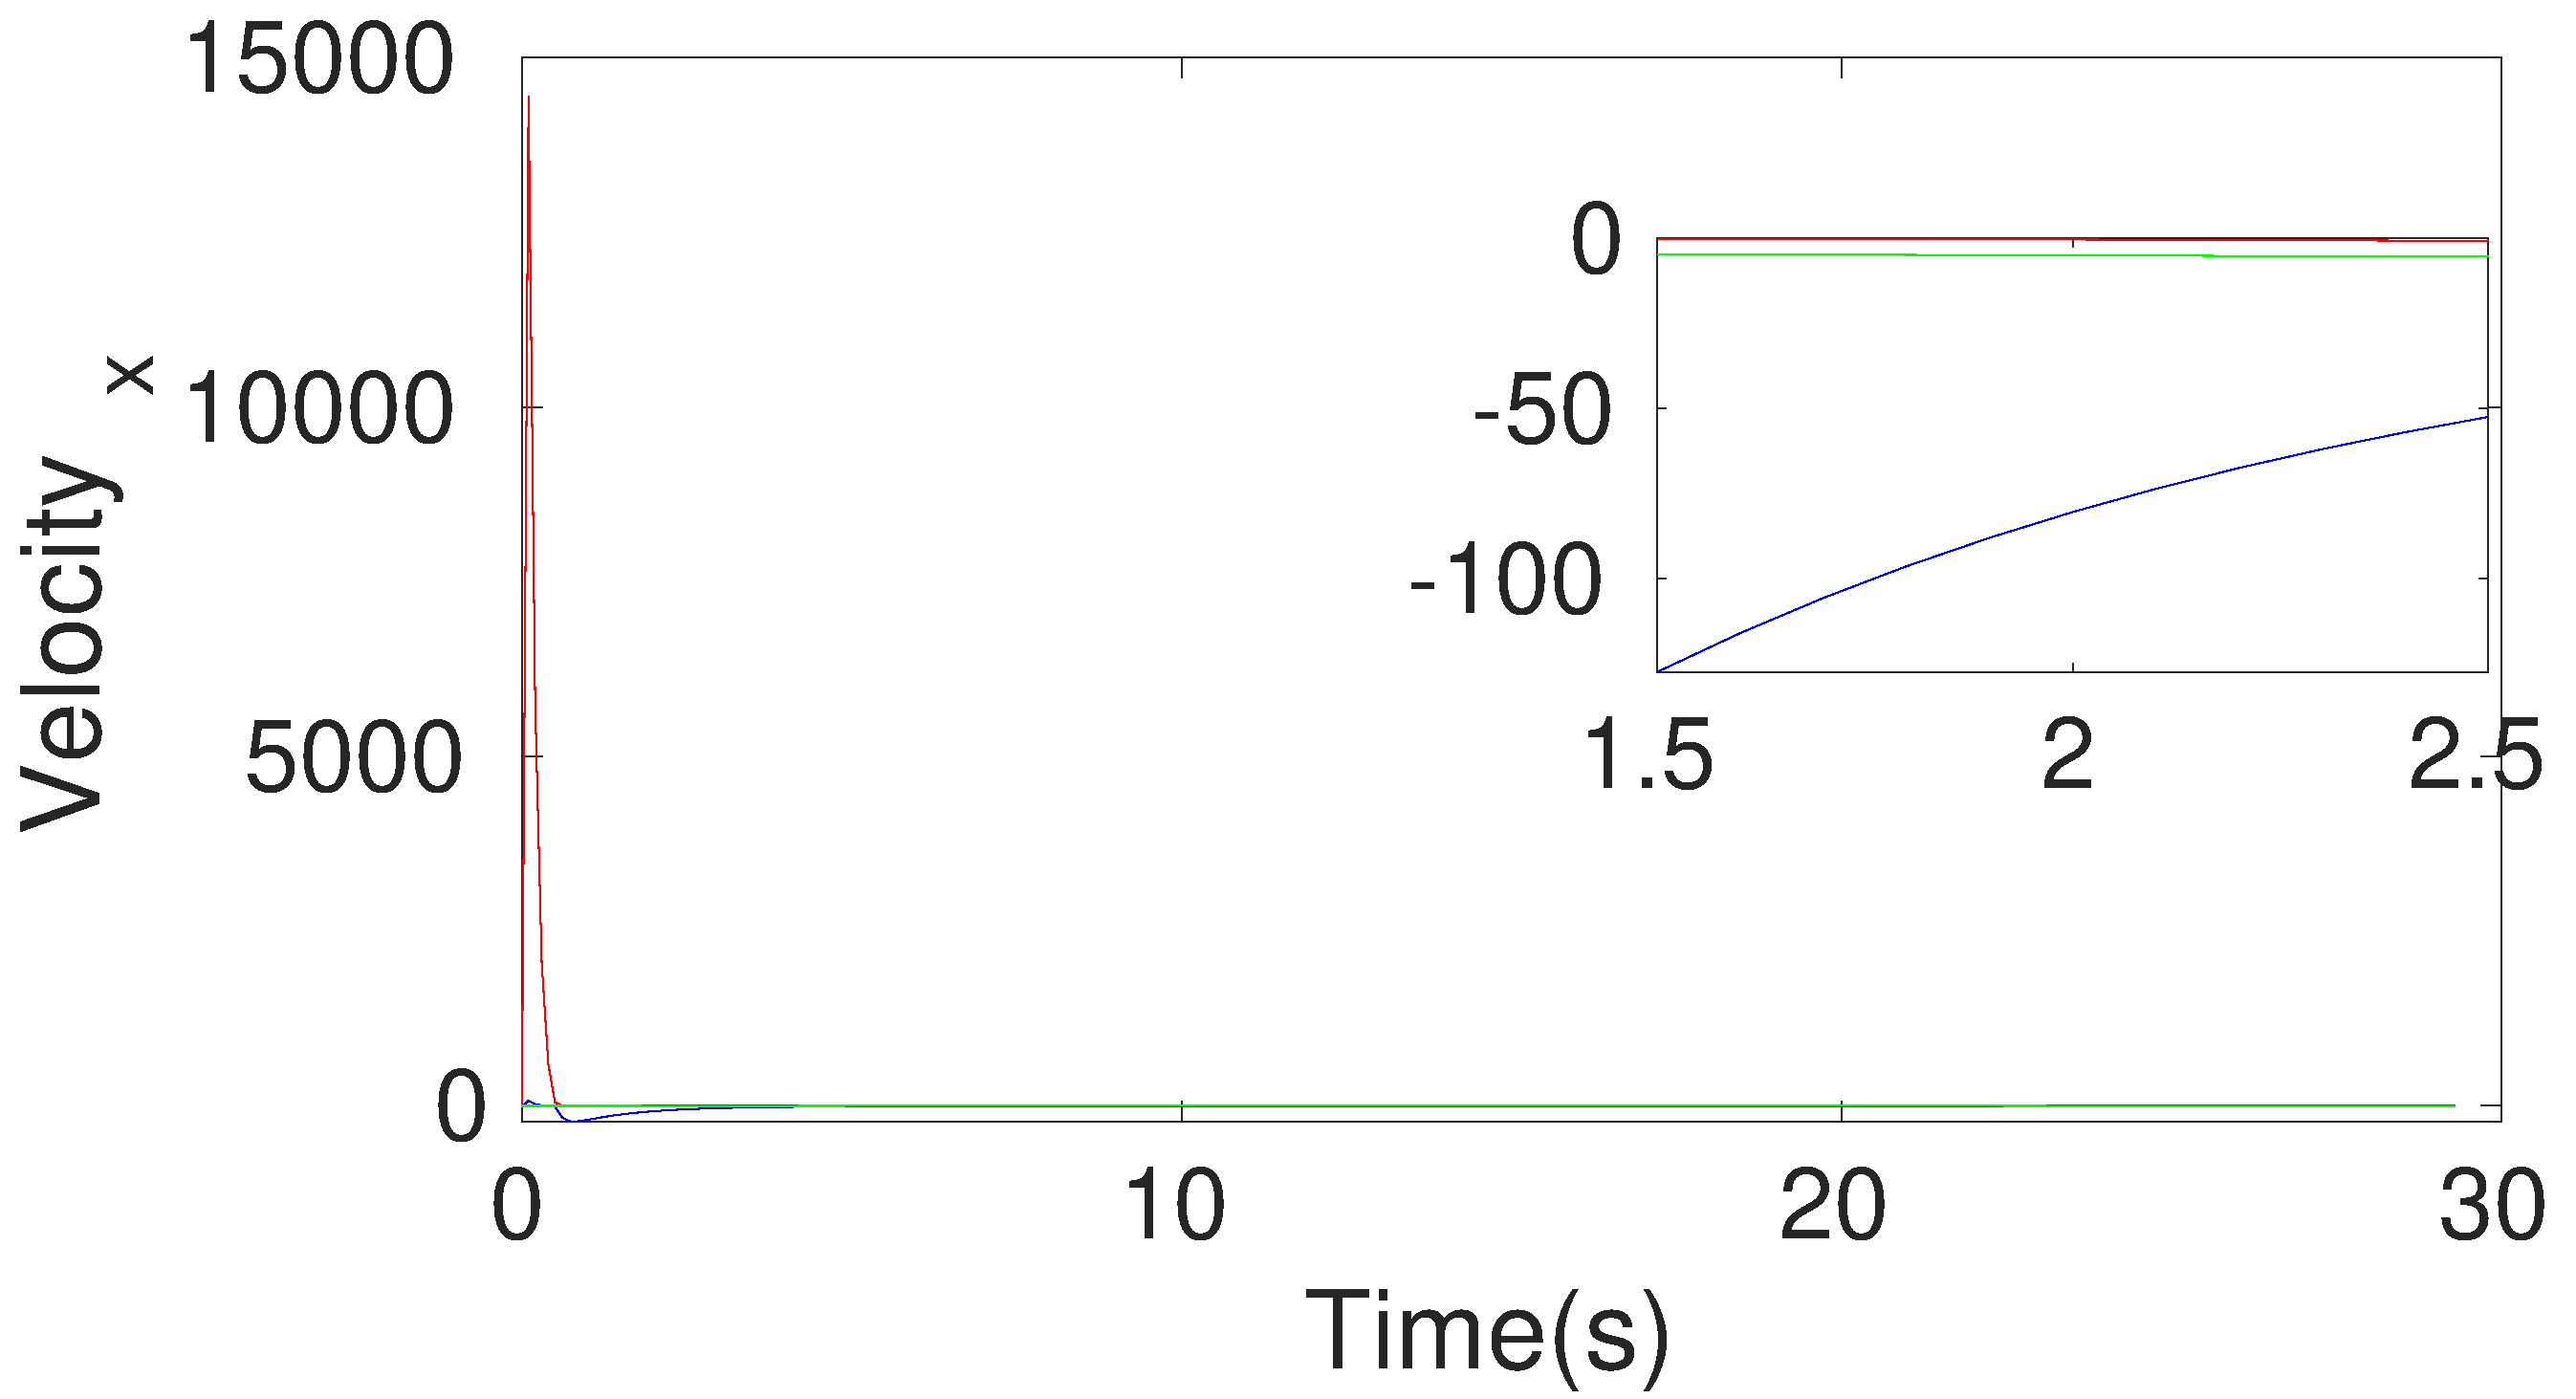
\includegraphics[width=.9\linewidth]{figures/HInf/s3caHInfVelocity_x}
\end{subfigure}
\begin{subfigure}{.5\linewidth}
\centering
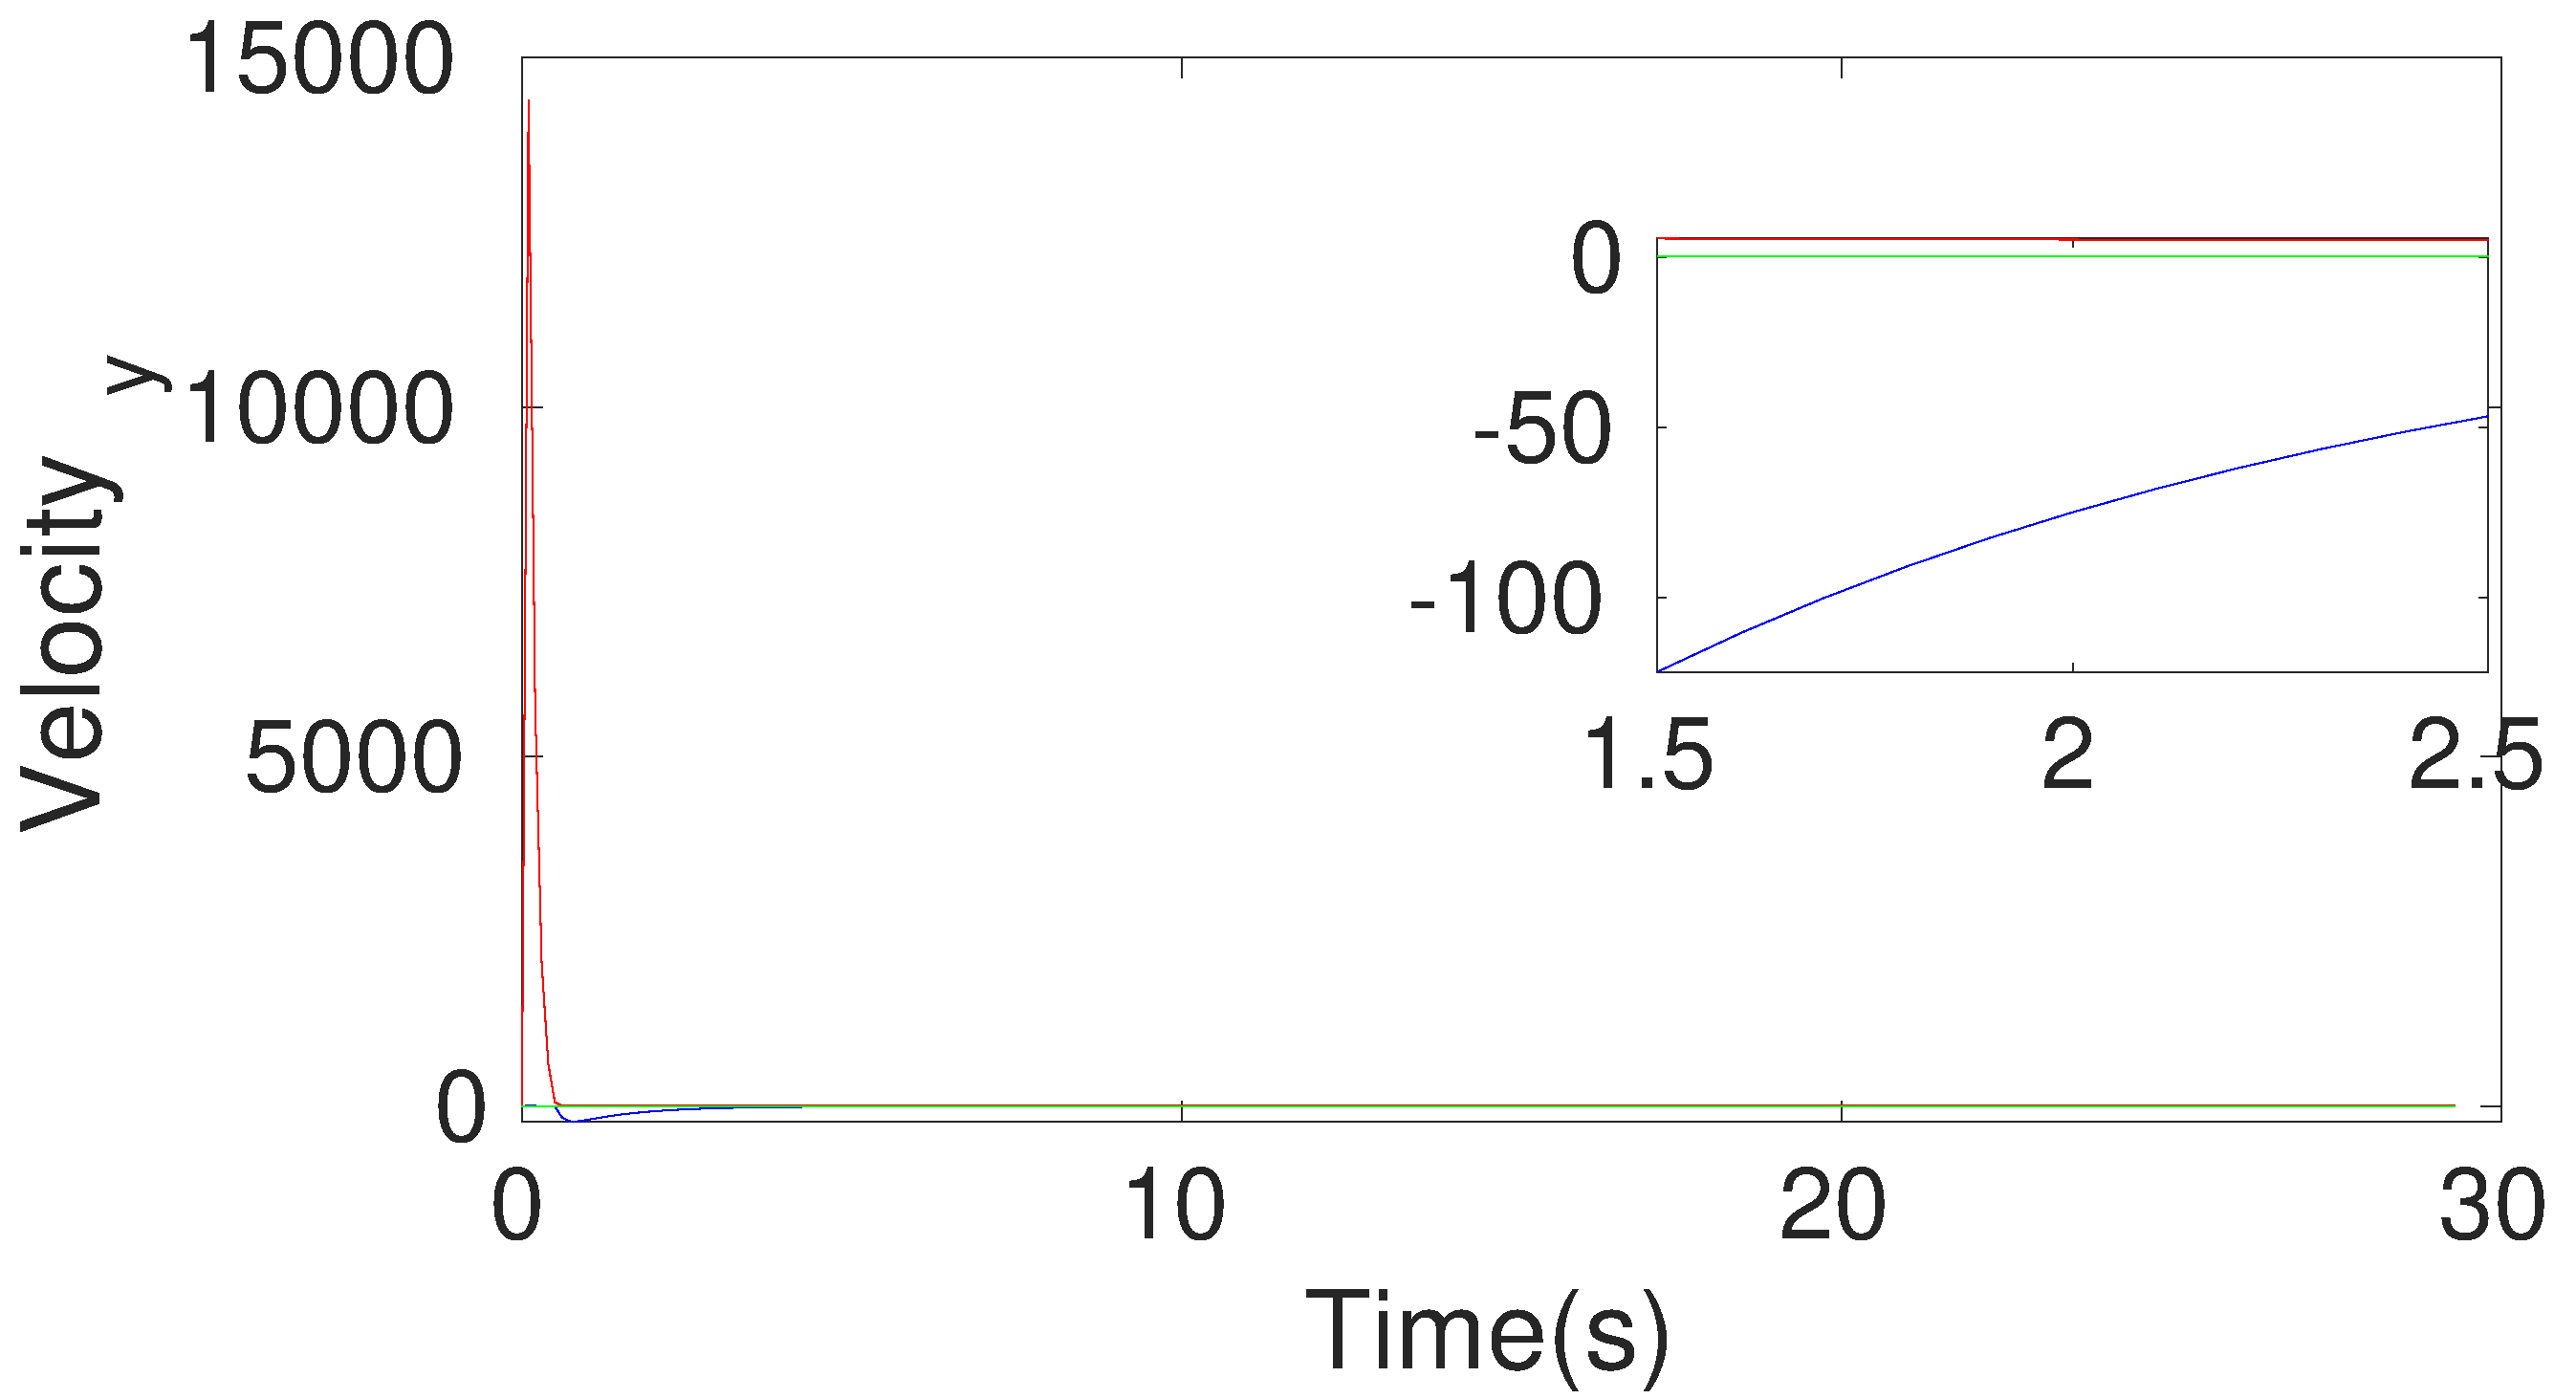
\includegraphics[width=.9\linewidth]{figures/HInf/s3caHInfVelocity_y}
\end{subfigure}
\begin{subfigure}{.5\linewidth}
\centering
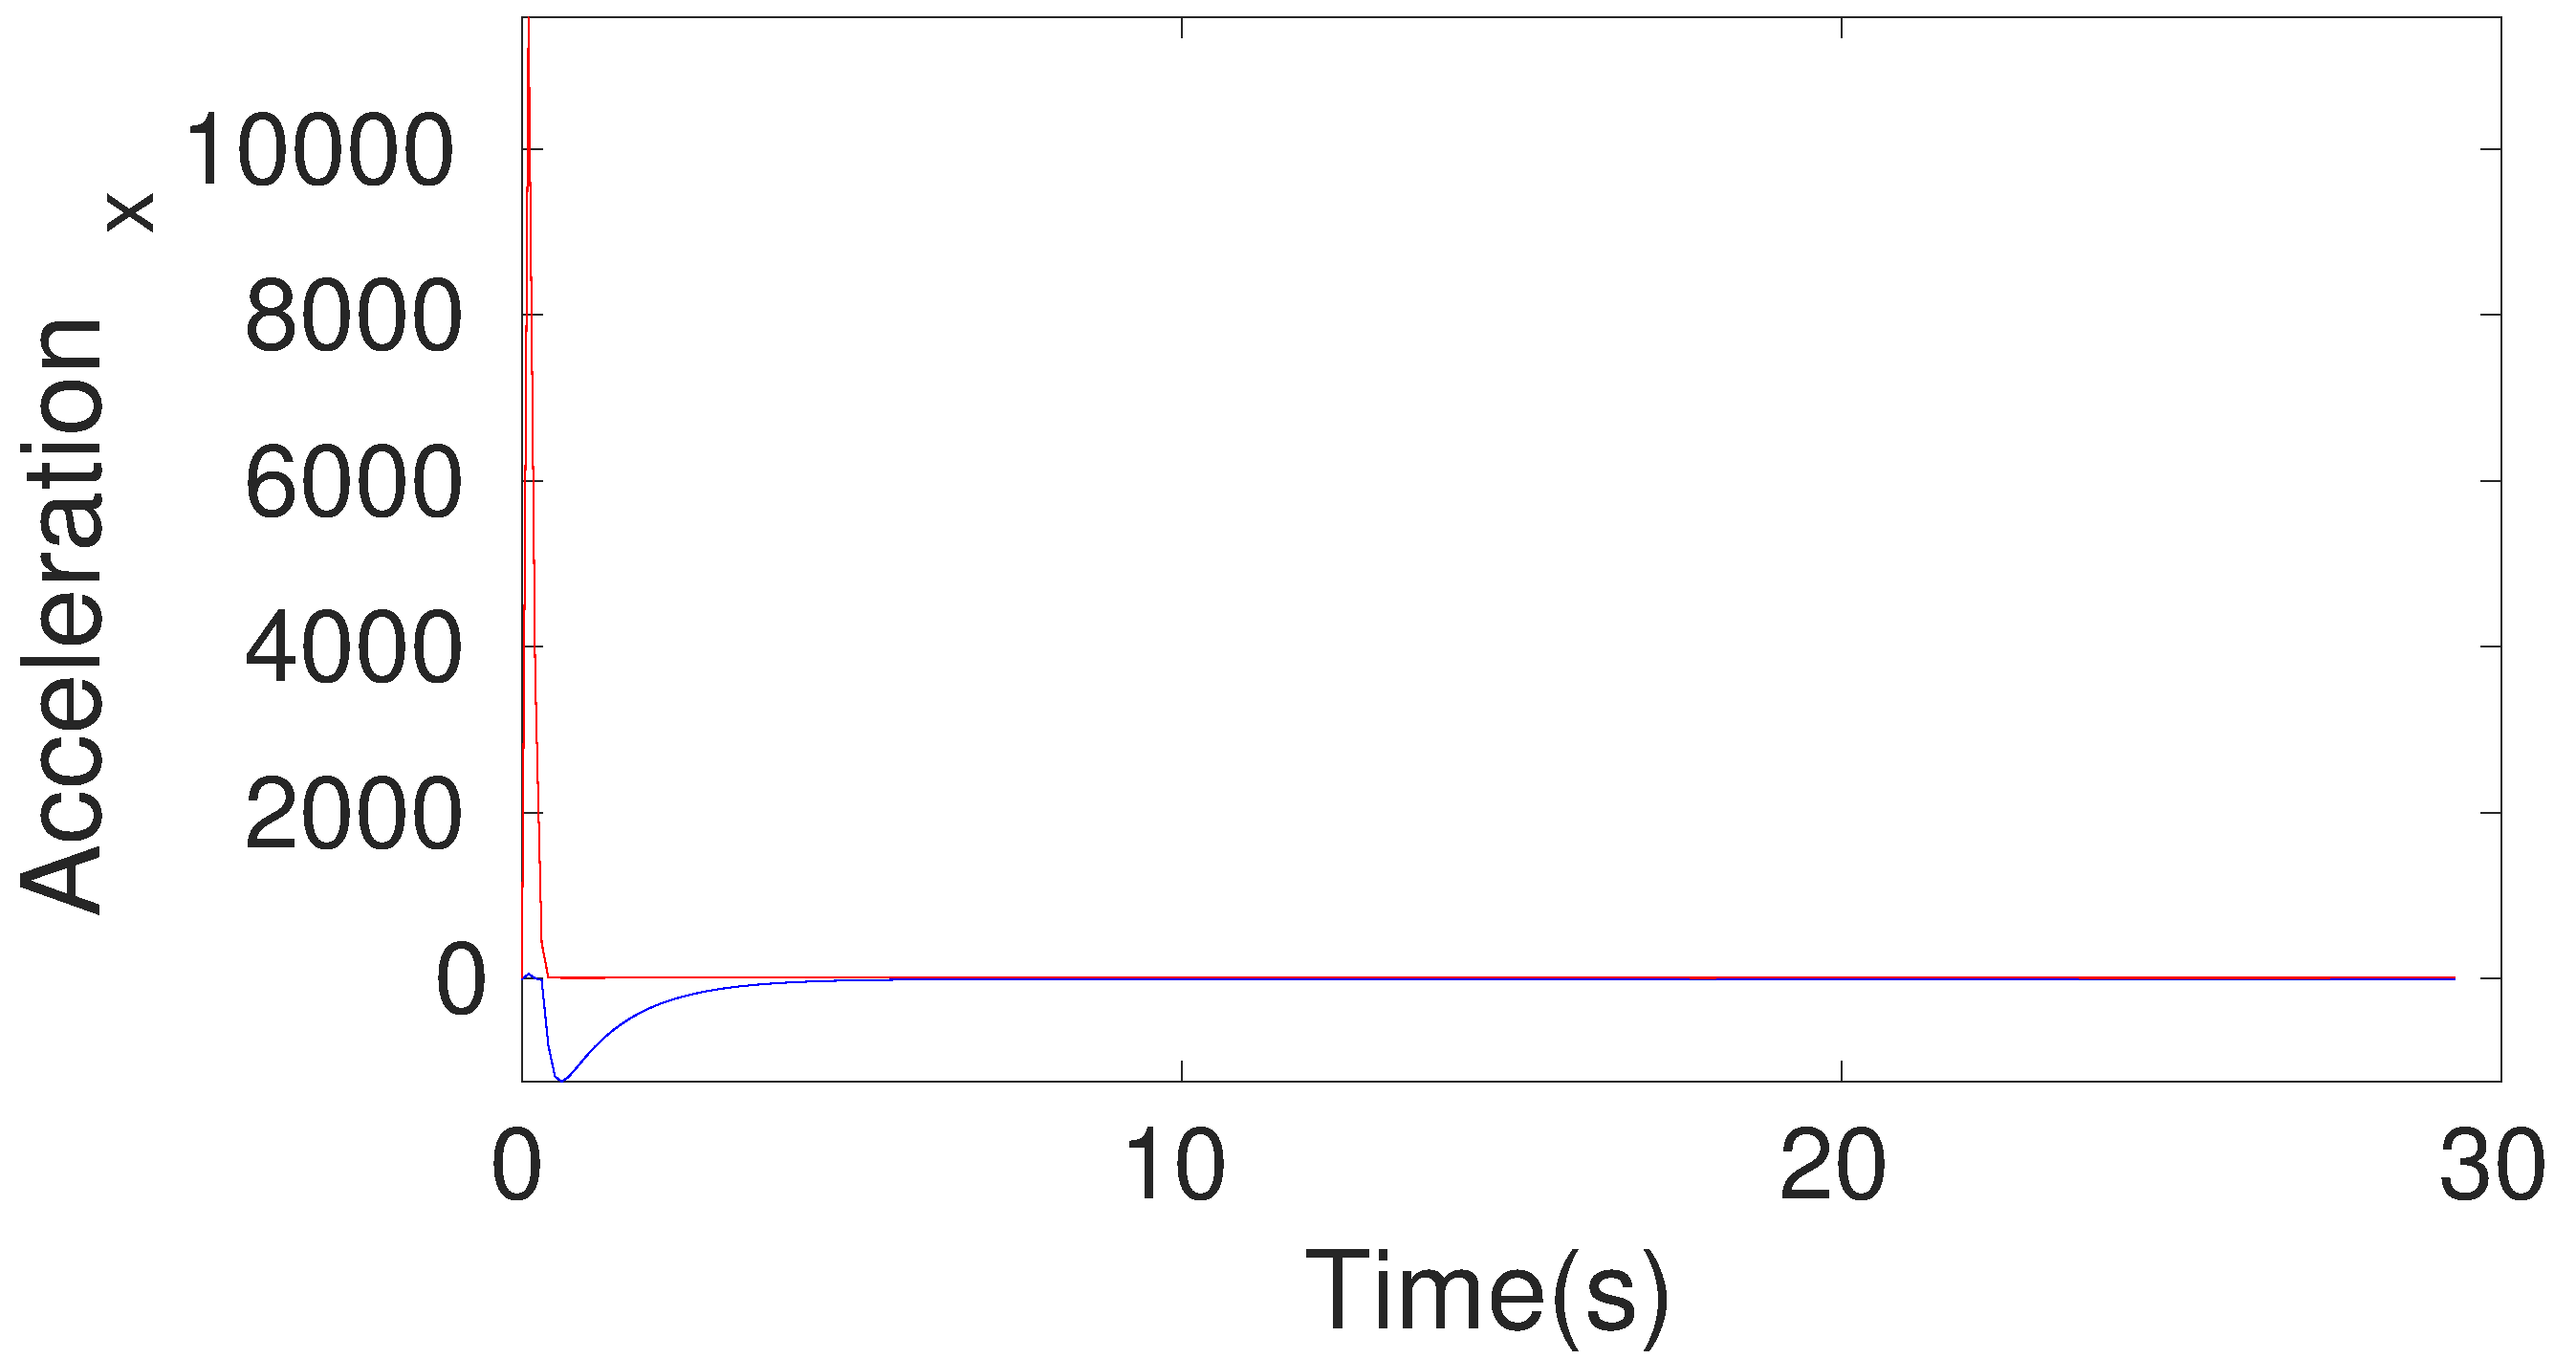
\includegraphics[width=.9\linewidth]{figures/HInf/s3caHInfAcceleration_x}
\end{subfigure}
\begin{subfigure}{.5\linewidth}
\centering
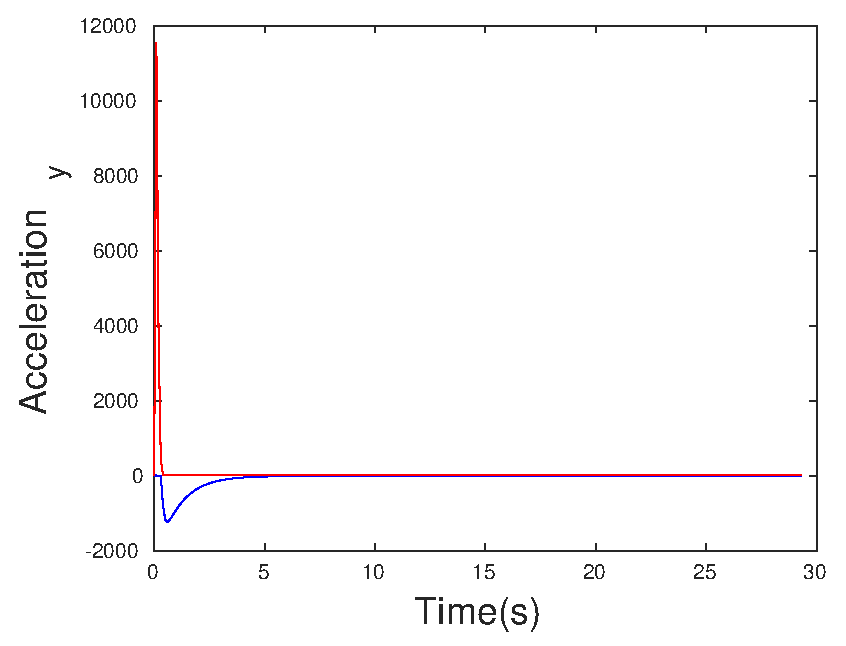
\includegraphics[width=.9\linewidth]{figures/HInf/s3caHInfAcceleration_y}
\end{subfigure}
\caption{Estimation using Constant Acceleration}
\end{figure}



\begin{figure}[h]
\begin{subfigure}{.5\linewidth}
\centering
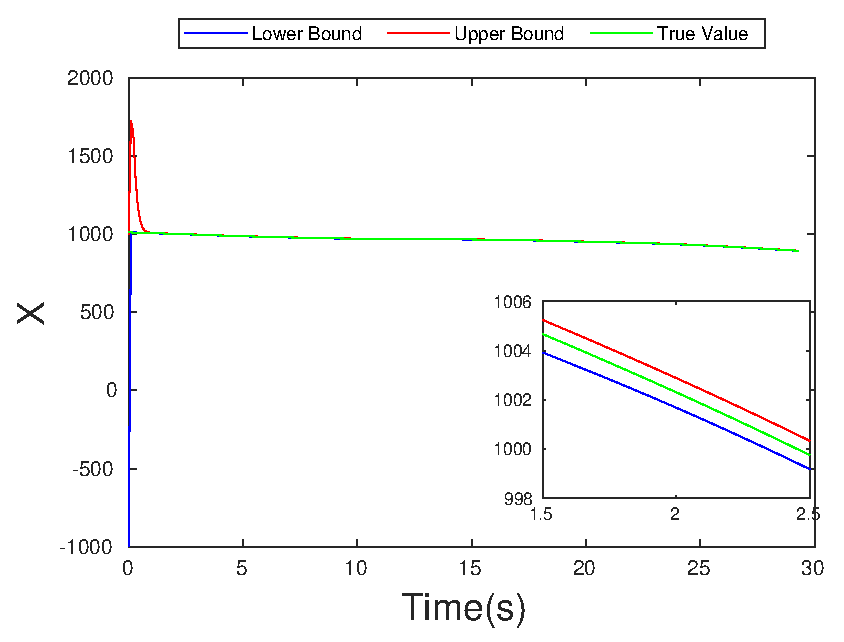
\includegraphics[width=\linewidth]{figures/HInf/s3csHInfX}
\end{subfigure}
\begin{subfigure}{.5\linewidth}
\centering
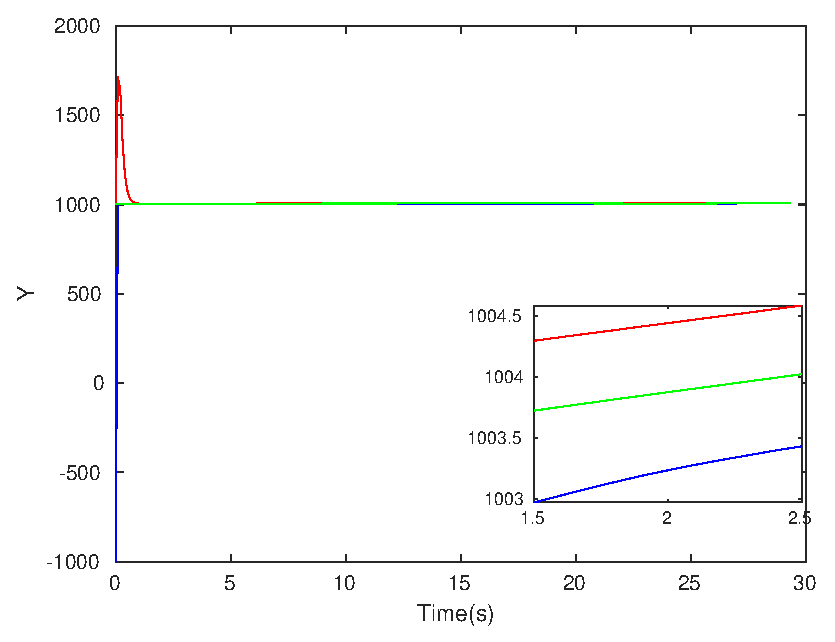
\includegraphics[width=\linewidth]{figures/HInf/s3csHInfY}
\end{subfigure}
\begin{subfigure}{.5\linewidth}
\centering
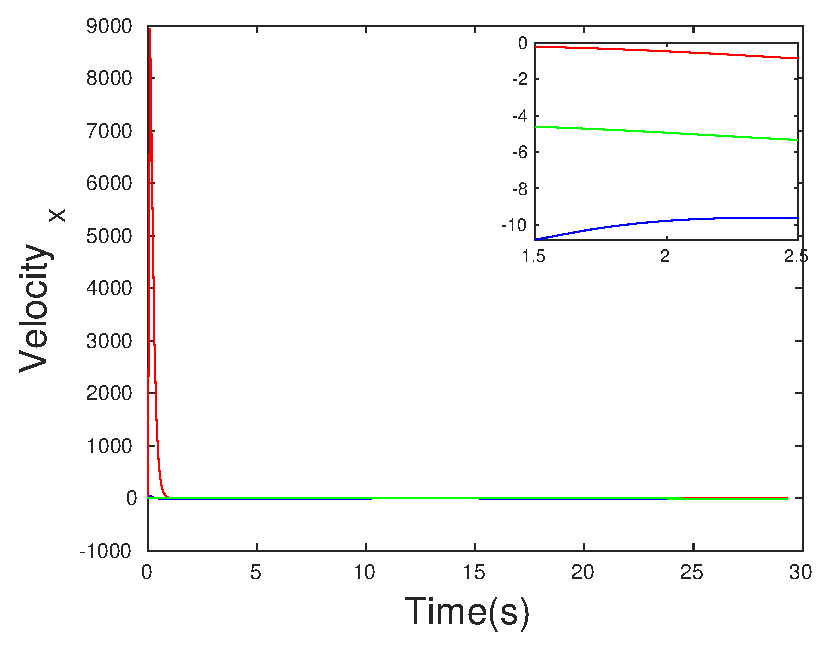
\includegraphics[width=.9\linewidth]{figures/HInf/s3csHInfVelocity_x}
\end{subfigure}
\begin{subfigure}{.5\linewidth}
\centering
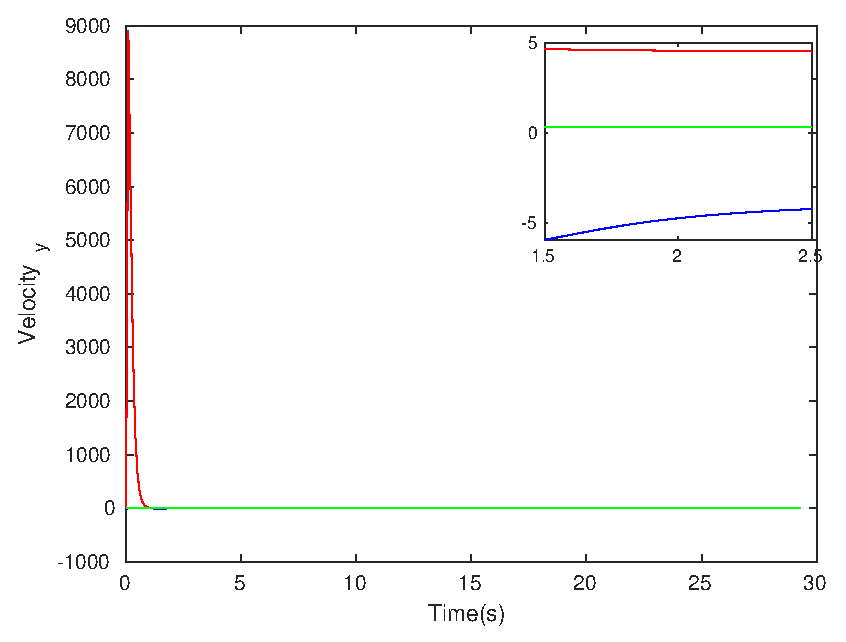
\includegraphics[width=.9\linewidth]{figures/HInf/s3csHInfVelocity_y}
\end{subfigure}
\begin{subfigure}{.5\linewidth}
\centering
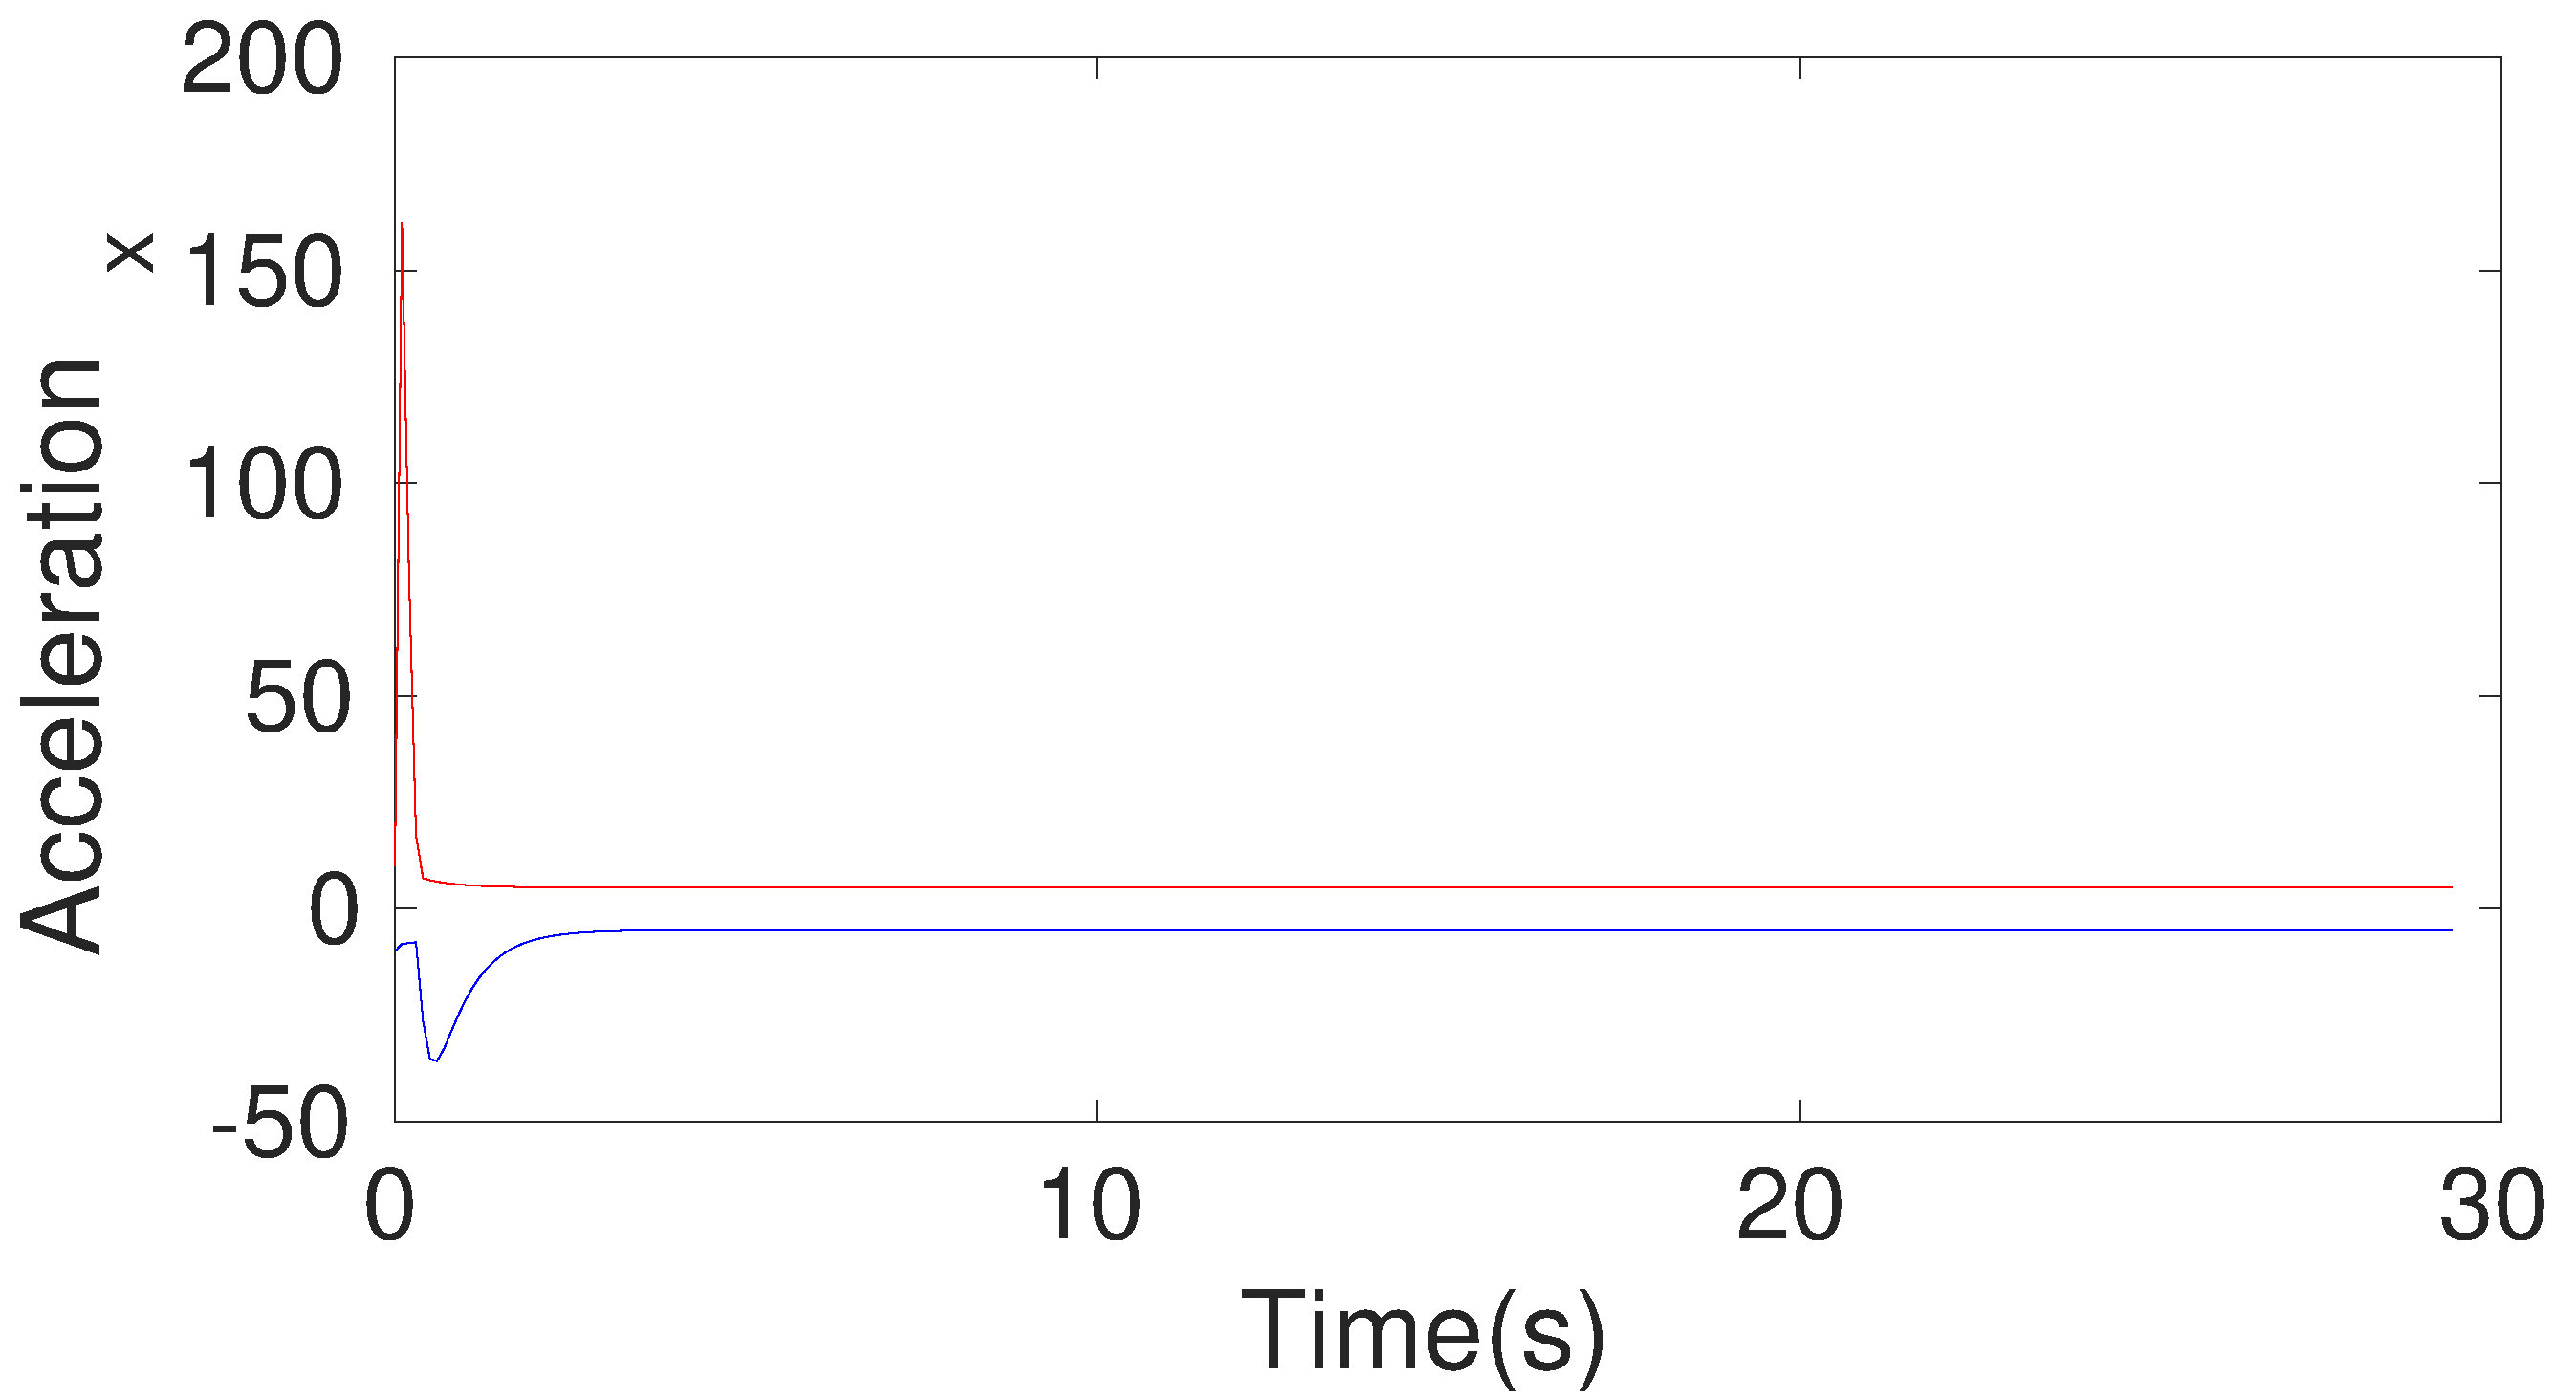
\includegraphics[width=.9\linewidth]{figures/HInf/s3csHInfAcceleration_x}
\end{subfigure}
\begin{subfigure}{.5\linewidth}
\centering
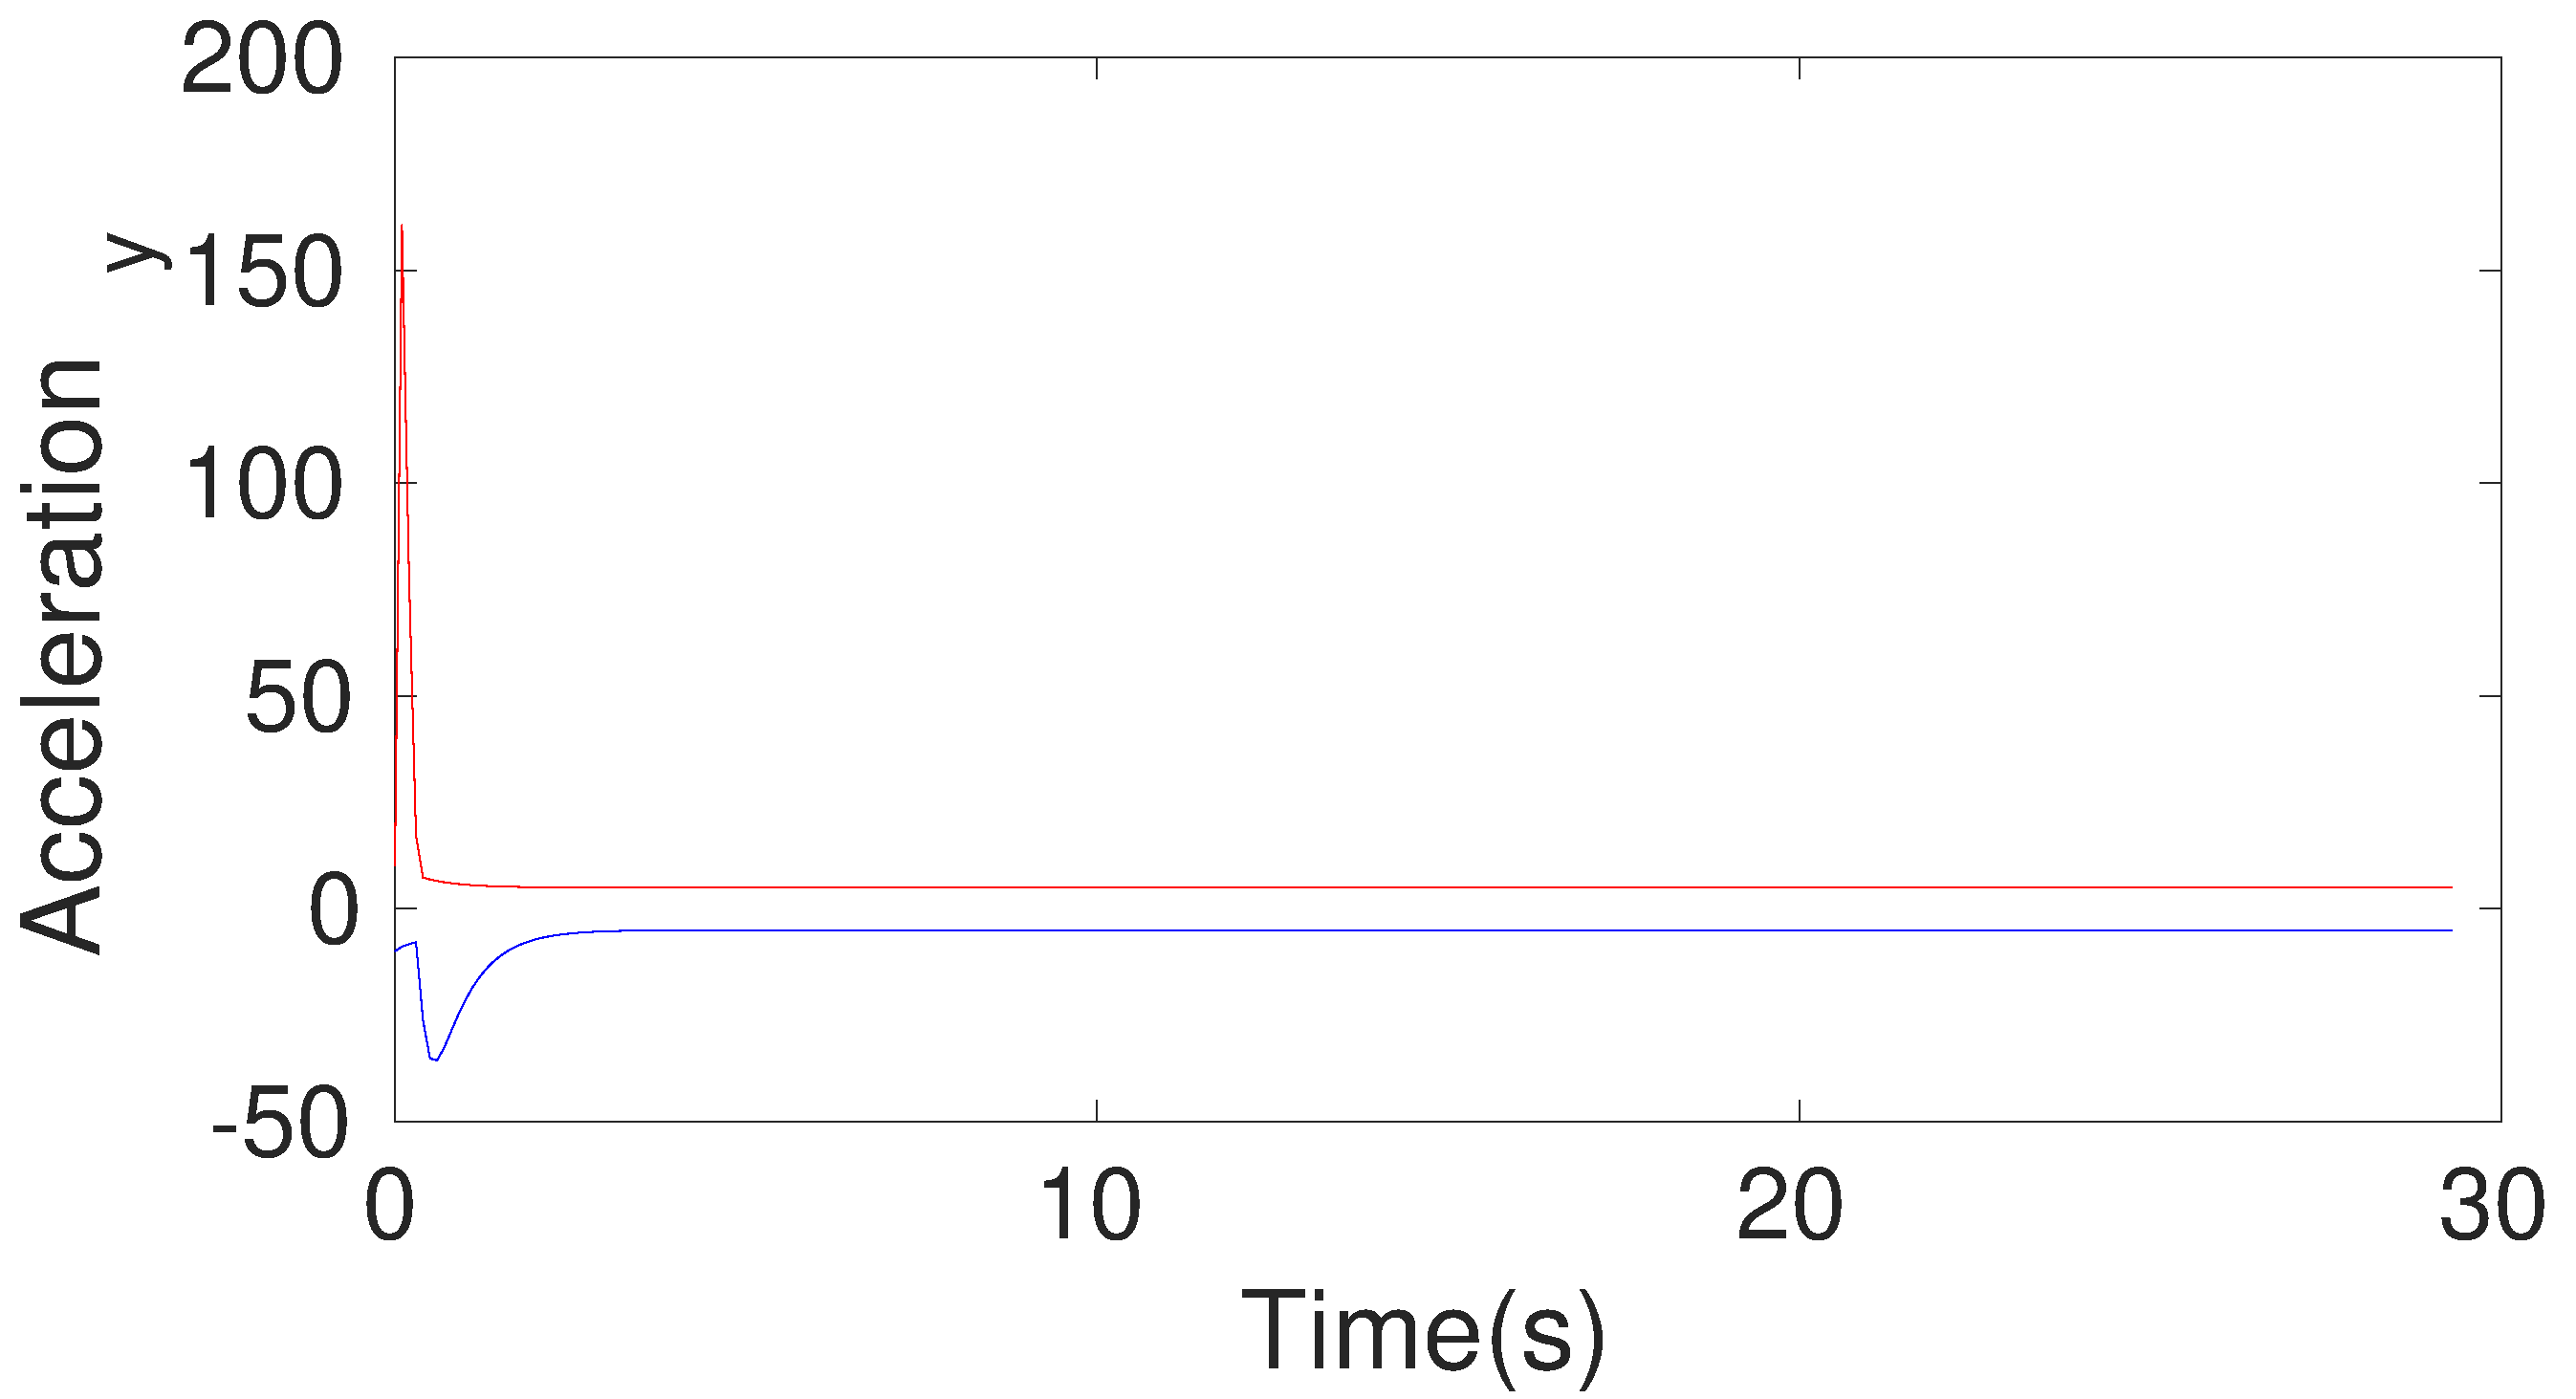
\includegraphics[width=.9\linewidth]{figures/HInf/s3csHInfAcceleration_y}
\end{subfigure}
\caption{Estimation using Singer Acceleration}
\end{figure}


\section{Rate of Change of Bounds}
\FloatBarrier
\subsection{Constant Velocity}
\begin{figure}[!h]
\begin{subfigure}{.5\linewidth}
\centering
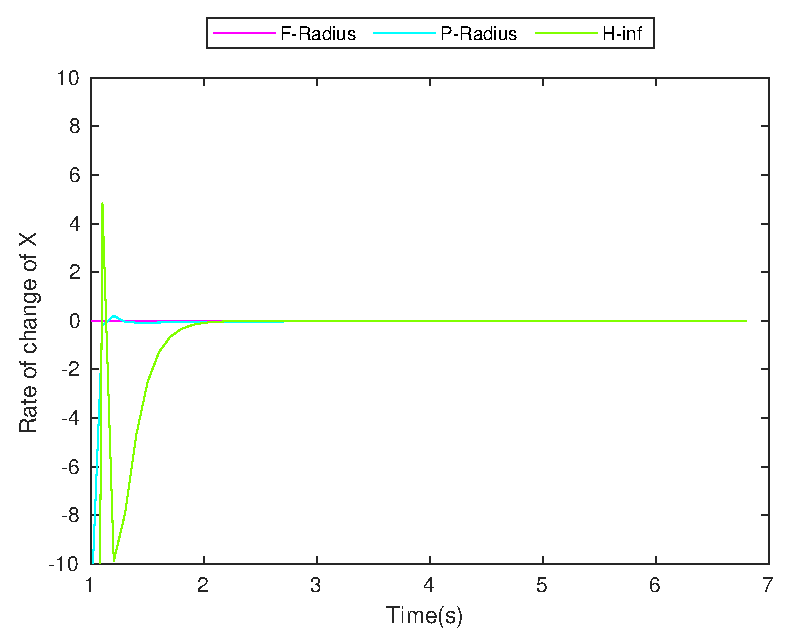
\includegraphics[width=\linewidth]{figures/BoundChange/CV/cv_bound_changeX}
\end{subfigure}
\begin{subfigure}{.5\linewidth}
\centering
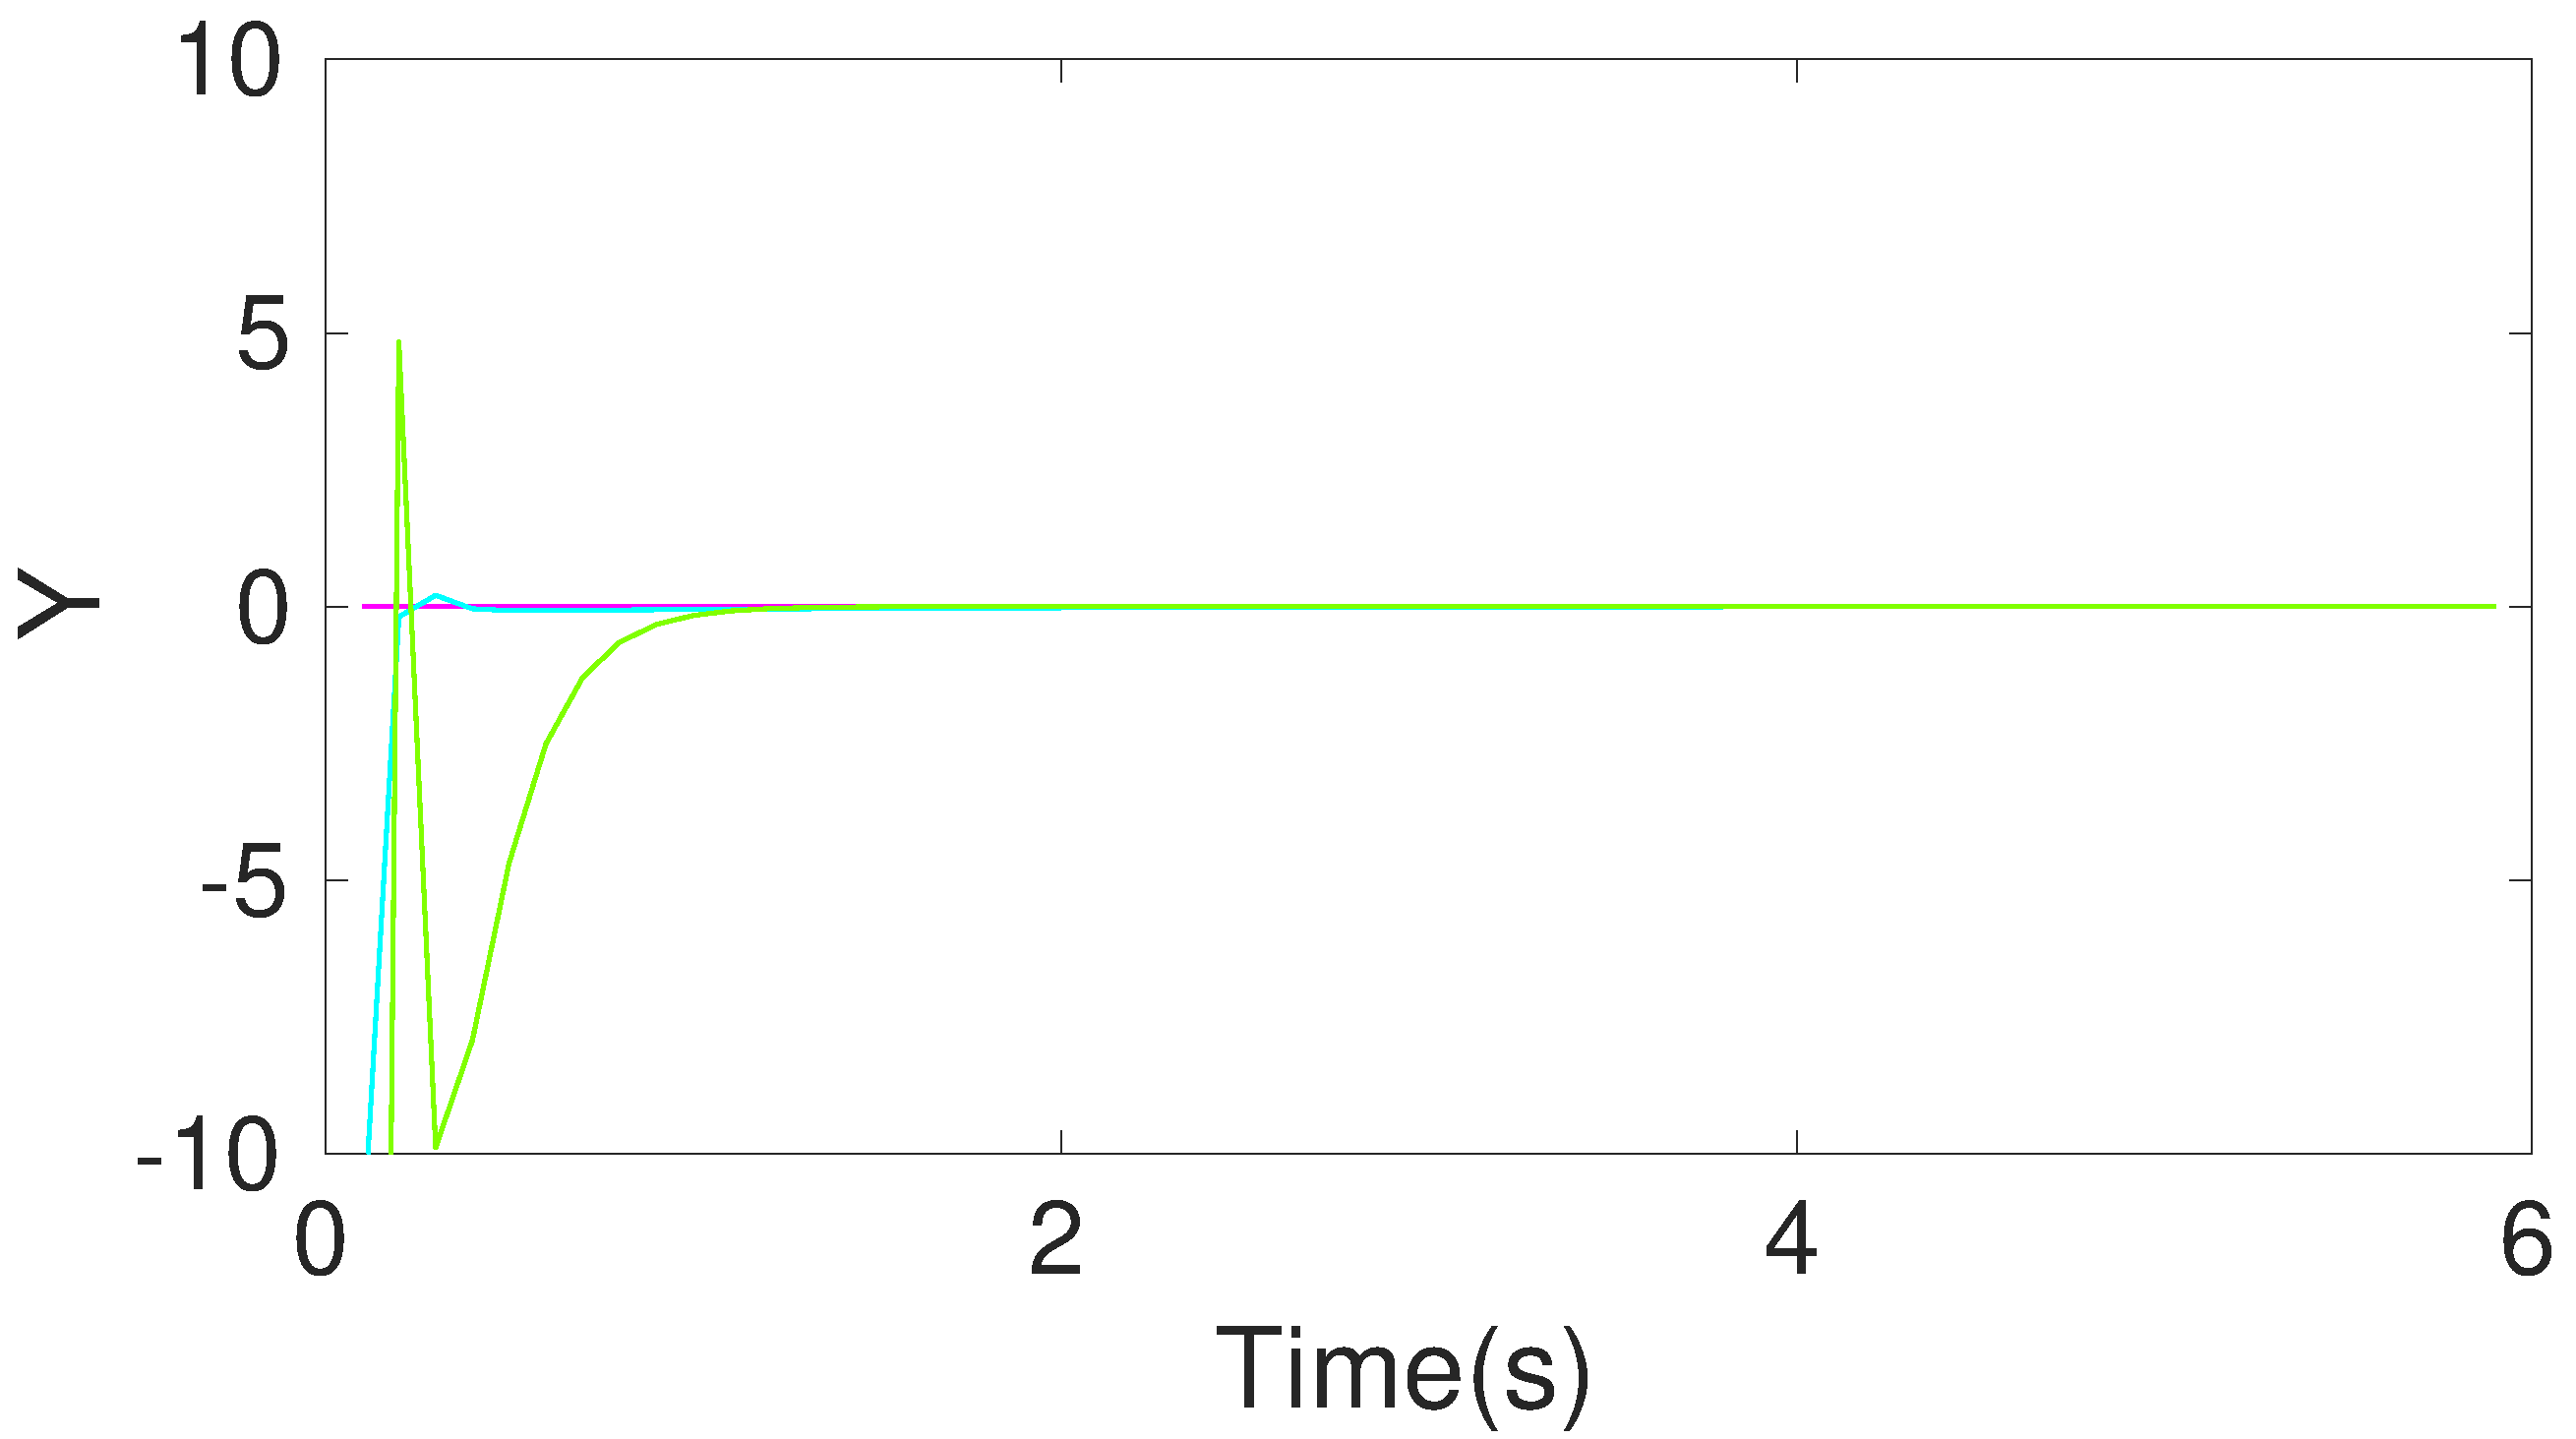
\includegraphics[width=\linewidth]{figures/BoundChange/CV/cv_bound_changeY}
\end{subfigure}
\begin{subfigure}{.5\linewidth}
\centering
\includegraphics[width=.9\linewidth]{figures/BoundChange/CV/cv_bound_changeVelocity_x}
\end{subfigure}
\begin{subfigure}{.5\linewidth}
\centering
\includegraphics[width=.9\linewidth]{figures/BoundChange/CV/cv_bound_changeVelocity_y}
\end{subfigure}
\caption{Rate of change of bounds}
\end{figure}

\subsection{Constant Acceleration}
\FloatBarrier
\begin{figure}[!h]
\begin{subfigure}{.5\linewidth}
\centering
\includegraphics[width=\linewidth]{figures/BoundChange/CA/ca_bound_changeX}
\end{subfigure}
\begin{subfigure}{.5\linewidth}
\centering
\includegraphics[width=\linewidth]{figures/BoundChange/CA/ca_bound_changeY}
\end{subfigure}
\begin{subfigure}{.5\linewidth}
\centering
\includegraphics[width=.9\linewidth]{figures/BoundChange/CA/ca_bound_changeVelocity_x}
\end{subfigure}
\begin{subfigure}{.5\linewidth}
\centering
\includegraphics[width=.9\linewidth]{figures/BoundChange/CA/ca_bound_changeVelocity_y}
\end{subfigure}
\begin{subfigure}{.5\linewidth}
\centering
\includegraphics[width=.9\linewidth]{figures/BoundChange/CA/ca_bound_changeAcceleration_x}
\end{subfigure}
\begin{subfigure}{.5\linewidth}
\centering
\includegraphics[width=.9\linewidth]{figures/BoundChange/CA/ca_bound_changeAcceleration_y}
\end{subfigure}
\caption{Rate of change of bounds}
\end{figure}

\subsection{Singer Acceleration Model}
\FloatBarrier
\begin{figure}[!h]
\begin{subfigure}{.5\linewidth}
\centering
\includegraphics[width=\linewidth]{figures/BoundChange/CS/cs_bound_changeX}
\end{subfigure}
\begin{subfigure}{.5\linewidth}
\centering
\includegraphics[width=\linewidth]{figures/BoundChange/CS/cs_bound_changeY}
\end{subfigure}
\begin{subfigure}{.5\linewidth}
\centering
\includegraphics[width=.9\linewidth]{figures/BoundChange/CS/cs_bound_changeVelocity_x}
\end{subfigure}
\begin{subfigure}{.5\linewidth}
\centering
\includegraphics[width=.9\linewidth]{figures/BoundChange/CS/cs_bound_changeVelocity_y}
\end{subfigure}
\begin{subfigure}{.5\linewidth}
\centering
\includegraphics[width=.9\linewidth]{figures/BoundChange/CS/cs_bound_changeAcceleration_x}
\end{subfigure}
\begin{subfigure}{.5\linewidth}
\centering
\includegraphics[width=.9\linewidth]{figures/BoundChange/CS/cs_bound_changeAcceleration_y}
\end{subfigure}
\caption{Rate of change of bounds}
\end{figure}